\documentclass[11pt,english, letter, amsmath]{article}
%2multibyte Version: 5.50.0.2890 CodePage: 1252

\usepackage{multibib}
\newcites{APP}{References}
\usepackage[usenames,dvipsnames]{xcolor}
\usepackage{placeins}
\usepackage{graphicx}
\usepackage{float}
\usepackage{subcaption}
\usepackage{adjustbox}
\usepackage{amsmath}
\usepackage{amsfonts}
\usepackage{booktabs}
\usepackage{bbold}
\usepackage{multirow}
\usepackage{setspace}
\usepackage{addlines}
\usepackage{comment}
\usepackage{array}
\usepackage{amssymb}
\usepackage{lscape}
\usepackage[authoryear]{natbib}
\usepackage{color}
\usepackage{chronology}     % Paquete para el timeline
\usepackage{booktabs}       % Paquete para mejorar el formato de las tablas
\usepackage{graphicx}       % Paquete para incluir y manipular gráficos
\usepackage{float} 
% Paquete para controlar la posición de las figuras y tablas
\usepackage[justification=centering]{caption}    
%\usepackage{breakurl}
\usepackage{rotating}
\usepackage{ textcomp }
\usepackage{tikz}
\usepackage[flushleft]{threeparttable}
\usepackage{framed}
\setcounter{MaxMatrixCols}{30}
\definecolor{parula3}{rgb}{0.2440,    0.4358,    0.9988}
\usepackage[colorlinks=true,citecolor=parula3,linkcolor=parula3,urlcolor=blue]{hyperref}
\usepackage{cleveref}
\usepackage{natbib}
\usepackage[a4paper,top=3cm,bottom=2cm,left=2.5cm,right=2.5cm,marginparwidth=1.75cm]{geometry}
\usepackage{booktabs}


% Default settings for table and figure captions
\usepackage{caption}
\captionsetup[table]{font=small,labelfont=small}
\captionsetup[figure]{font=small,labelfont=small}

% Float spacing adjustments to reduce blank spaces and distribute figures evenly
\setlength{\textfloatsep}{6pt plus 2pt minus 2pt}  % Space between text and floats
\setlength{\floatsep}{8pt plus 2pt minus 2pt}       % Space between consecutive floats
\setlength{\intextsep}{6pt plus 2pt minus 2pt}      % Space between inline floats and text
\renewcommand{\floatpagefraction}{0.75}             % Allow 75% of page for floats
\renewcommand{\topfraction}{0.85}                   % Allow 85% of top for floats
\renewcommand{\bottomfraction}{0.75}                % Allow 75% of bottom for floats
\renewcommand{\textfraction}{0.15}                  % Require at least 15% text on page
\setcounter{topnumber}{3}                           % Max 3 floats at top
\setcounter{bottomnumber}{2}                        % Max 2 floats at bottom
\setcounter{totalnumber}{4}                         % Max 4 floats per page

% Reduce paragraph spacing and increase penalties for whitespace
\setlength{\parskip}{2pt plus 0pt minus 0pt}        % Minimal paragraph skip
\clubpenalty=9999                                   % Prevent orphaned lines (strong penalty)
\widowpenalty=9999                                  % Prevent widows (strong penalty)
\displaywidowpenalty=9999                           % Penalty for display math widows
\brokenpenalty=9999                                 % Penalty for breaking lines

\newcommand\mythanks[1]{%
  \begingroup
  \renewcommand\thefootnote{}\footnote{#1}%
  \addtocounter{footnote}{-1}%
  \endgroup
}


\newtheorem{claim}{{\bf \sc Claim}}
\newtheorem{theorem}{{\bf \sc Theorem}}
\newtheorem{lemma}{{\bf \sc Lemma}}
\newtheorem{example}{{\bf \sc Example}}
\newtheorem{definition}{{\bf \sc Definition}}
\newtheorem{corollary}{{\bf \sc Corollary}}
\newtheorem{proposition}{{\bf \sc Proposition}}
\newtheorem{remark}{{\bf \sc Remark}}
\def \Re{\mathbb{R}}
\def \eproof{\hbox{\hskip3pt\vrule width4pt height8pt depth1.5pt}}
\newenvironment{proof}[1][Proof]{\noindent \textbf{#1.} }{\  \rule{0.5em}{0.5em}}

\renewcommand{\baselinestretch}{1.2}
\newcommand*{\QEDA}{\hfill\ensuremath{\blacksquare}}%

\newcommand{\xxx}[2][show]{ % Replace "show" with any other word to hide XXX comments.
\ifthenelse{\equal{#1}{show} }{ \textcolor{purple}{X #2 X}}{}}

\usepackage{soul}
\usepackage{endnotes}
\usepackage[colorinlistoftodos]{todonotes}

\addtocontents{toc}{\protect\setcounter{tocdepth}{0}}

\usepackage{tikz}
\usetikzlibrary{shapes,arrows}
\usetikzlibrary{calc,decorations.pathmorphing,decorations.text,fixedpointarithmetic}
\usetikzlibrary{decorations.pathreplacing,calligraphy}


\newcommand{\cmark}{\text{\ding{51}}}
\newcommand{\xmark}{\text{\ding{55}}}


%\DeclarePairedDelimiter\floor{\lfloor}{\rfloor}

%----------------------------------------------------------------------------------------------------------
% BIBLIOGRAPHY
\usepackage[authoryear]{natbib}
\renewcommand{\cite}{\citet}
\setcounter{MaxMatrixCols}{10}

%External appendices
\usepackage{xr-hyper}

\makeatletter
\newcommand*{\addFileDependency}[1]{% argument=file name and extension
  \typeout{(#1)}
  \@addtofilelist{#1}
  \IfFileExists{#1}{}{\typeout{No file #1.}}
}
\makeatother

\newcommand*{\myexternaldocument}[1]{%
    \externaldocument{#1}%
    \addFileDependency{#1.tex}%
    \addFileDependency{#1.aux}%
}

\myexternaldocument{Appendices}

%Theorems
%\newtheorem{example}{Example}
%\newtheorem{assume}{Assumption}
%\newtheorem{proposition}{Proposition}
%\newtheorem{lemma}{Lemma}
%\newtheorem{corollary}{Corollary}
%\newtheorem{theorem}{Theorem}
%\newtheorem{definition}{Definition}

\newcommand{\jr}[1]{\textcolor{blue}{#1}} %Color para revision Profe Jorge

\newcommand{\pa}[1]{\textcolor{violet}{#1}} %Color para revision Patricio

\newcommand{\dc}[1]{\textcolor{red}{#1}} %Color para revision Dante Contreras

\newcommand{\ps}[1]{\textcolor{brown}{#1}} %Color para revision Paulina


\setcounter{section}{0}
\makeindex
\newcommand{\notindep}{\ensuremath{\perp\!\!\!\!\!\!\diagup\!\!\!\!\!\!\perp}}
\DeclareMathOperator*{\argmin}{argmin}


%----------------------------------------------------------------------------------------------------------
% HYPER-REFERENCES CONFIGURATION - PDF
%----------------------------------------------------------------------------------------------------------

\hypersetup{
colorlinks=true,linkcolor=blue,citecolor=blue, filecolor=magenta, citebordercolor=yellow,
linkbordercolor = magenta,
}

\begin{document}
\raggedbottom
\thispagestyle{empty}\setcounter{page}{0}
\vspace*{.2in}

\begin{center}
\textbf{\Large Boots in the Beat: Effects of Beat Policing on Victimization and Crime Perception}$^\dagger$
\end{center}
\vspace{.25in}

\begin{center}\large
  Andr\'es Barrios-Fern\'andez \hspace{.12in}
  Jorge Garc\'ia-Hombrados \hspace{.12in}
  Daniel P\'erez-Parra
\end{center}

\medskip

\begin{center}\large
\today \\
\href{https://andresbarriosf.github.io/police_reform.pdf}{Latest Version}
\end{center}

\mythanks{\hspace{-.25in}$^\dagger$
Corresponding author: Andrés Barrios-Fernández (andres.bafer@alumni.lse.ac.uk). School of Business and Economics. Universidad de los Andes, Chile. Monseñor Álvaro del Portillo 12.455. Las Condes. Santiago. We thank Carabineros de Chile for granting us access to the administrative data we use in this project. Andr\'es Barrios-Fernández acknowledges the financial support of Fondecyt Regular Project 1261817. Supplemental materials are available in the \href{https://andresbarriosf.github.io/online_appendix_police_reform.pdf}{Online Appendix}.}

\vspace{0.1in}

\begin{abstract}
\begin{quote}
%This paper provides causal evidence on the effects of beat policing on public security and police effectiveness. Using rich administrative and survey data from Chile, we study \emph{Plan Cuadrante}, a reform that shifted policing toward a beat-policing model by subdividing urban municipalities into smaller geographic units---i.e., quadrants---and permanently assigning each officer to one quadrant rather than rotating officers across the municipality. Exploiting the staggered implementation of the program across municipalities, we find large improvements across multiple outcomes. Among surveyed households, twelve-month victimization rates declined by 10 percentage points (36\%), and administrative records show a 10\% decline in crimes reported to the police. The reform also improved security perceptions. The share of households perceiving increased criminal activity fell by 15 percentage points (36\%), and, consistent with this pattern, household investment in private security measures declined by 7.7 percentage points (37\%). In some municipalities, implementation of \emph{Plan Cuadrante} was accompanied by significant increases in police resources. However, our mechanism analyses indicate that our findings are not driven by resource increases alone. The beat-policing components of the reform---i.e., permanent officer assignment and greater local knowledge---appear to be key to reducing crime and improving security perceptions.
This paper provides causal evidence on the effects of beat policing on public security and police effectiveness. Using rich administrative and survey data from Chile, we study \emph{Plan Cuadrante}, a reform that shifted policing toward a beat-policing model by subdividing urban municipalities into smaller geographic units---i.e., quadrants---and permanently assigning officers to these quadrants rather than rotating officers across the municipality. Exploiting the staggered implementation of the program across municipalities, we find large improvements in both public safety and security perceptions. Among surveyed households, twelve-month victimization rates declined by 10 percentage points (36\%), and administrative records show a 10\% decline in crimes reported to the police. Arrests increased by 14\% even as crime declined. The reform also improved security perceptions. The share of households perceiving increased criminal activity fell by 15 percentage points (36\%), and, consistent with this pattern, household investment in private security measures declined by 7.7 percentage points (37\%). In some municipalities, implementation of \emph{Plan Cuadrante} was accompanied by significant increases in police resources. However, our mechanism analyses indicate that our findings are not driven by resource increases alone, as they remain sizeable in municipalities with resource increases similar to those in control municipalities. The beat-policing components of the reform---i.e., permanent officer assignment and greater local knowledge---appear to be key to reducing crime and improving security perceptions.
\\[12pt]
\noindent\textbf{Keywords:} police strategy, beat policing, territorial deployment.\\
%\textbf{JEL codes:} 

\end{quote}
\end{abstract}



\clearpage


%\onehalfspacing
\doublespacing

\section{Introduction}
\label{introduction}
Crime imposes significant social costs, straining the criminal justice system and increasing both public and private security expenditures. Given these stakes, crime consistently ranks among the public's top concerns and features prominently in political debate \citep{Scartascini, gallup2023}. Police forces play a central role in controlling crime and maintaining public safety. While there is extensive evidence on the effects of police resources on crime \citep[see, for instance,][]{Chalfin_JEL,Levitt_1997,DiTella}, we know much less about how the deployment of those resources, and the strategy changes enabled by different territorial assignments, shape police effectiveness. Studies of public service provision show that decentralization and local specialization can improve performance by aligning operations with local needs \citep[see, for instance,][]{besley2003centralized}. This suggests that policing models that foster local knowledge and allow officers to adapt practices to local conditions may be more effective. Beat policing reflects these insights. Rather than rotating officers across large areas, it permanently assigns each officer to a smaller territorial unit, enabling the accumulation of local knowledge and adaptation to local crime patterns and community dynamics \citep{cordner1995community,skogan1997comminuty}. This model has become increasingly common across police departments worldwide \citep{NASEM2018,PCSP2014}. Yet despite its widespread adoption, rigorous causal evidence on its effects on public safety and security perceptions remains scarce.

This paper combines rich administrative and survey data from Chile to provide causal evidence that beat policing can significantly improve public security and police effectiveness along multiple dimensions. We exploit quasi-random variation from the staggered adoption of a large reform, \emph{Plan Cuadrante}, which introduced a beat-policing model in urban areas by dividing police operational areas---typically municipalities---into smaller zones---quadrants---and permanently assigning officers to them. This permanent assignment was designed to help officers accumulate local knowledge of territorial features, crime patterns, and communities, and to adapt their practices accordingly. Using a difference-in-differences strategy, we show that adopting municipalities experienced significant declines in victimization, reported crime, and perceived insecurity.

\emph{Plan Cuadrante} was implemented in municipalities with at least 70\% urban population and rolled out between 1998 and 2013 across the 150 municipalities that met this condition. Its central objective was to reduce victimization and insecurity perceptions. Rather than changing police hierarchy or operational doctrine, the reform reorganized frontline deployment by subdividing police operational areas---typically municipalities---into quadrants and permanently assigning officers to each of them.
On average, municipalities were divided into seven quadrants, with size and boundaries defined by local police authorities based on road networks, geographic features, and available resources.

To examine the effects of \emph{Plan Cuadrante}, we use household-level data from the National Urban Security Survey (ENUSC), which reports crime victimization, security perceptions, trust in police, and private security investment for roughly 25,000 urban households across 101 municipalities each year. We complement these data with administrative records on arrests and crimes reported to the police. To leverage staggered adoption, we employ a difference-in-differences strategy comparing early and late adopters using the procedure developed in \citet{Callaway}. Analyses based on survey data focus on 46 urban municipalities that adopted the program between 2005 and 2012 and one never-treated municipality; together, they represent over one-quarter of Chile's population. Analyses based on administrative data use a broader sample of 96 municipalities that adopted between 2003 and 2013 and 196 never-treated municipalities, representing over half of Chile's population.

We find that households in adopting municipalities become 10 percentage points (36\%) less likely to experience crime in the previous 12 months, with effects appearing within one year and growing over time. Consistent with this finding, we document a 10\% decline in crimes reported to the police. These estimates may understate the reform's true impact because not all crimes are reported and, by bringing police closer to communities, the program could have increased reporting rates. Nevertheless, the alignment between survey-based and administrative estimates provides reassuring evidence of the reform's effectiveness.

Beyond reducing crime, the reform also reduced insecurity perceptions and private investment in security. This is noteworthy because actual crime and crime perceptions can diverge, potentially leading to suboptimal security expenditures. For example, \citet{Ajzenman_Pato} show that rising immigration in Chile between 2000 and 2016 did not increase crime but did increase insecurity perceptions.

A potential identification concern is that crime reductions in adopting municipalities could reflect displacement to neighboring areas rather than genuine effectiveness gains. Hot-spot policing, which concentrates police resources in high-crime locations, has been shown to generate this type of spatial displacement \citep{Blattman_Tobon_JEEA}. In our setting, spillovers are less likely because municipalities are large geographic areas and beat policing reorganized deployment across the full municipal territory rather than concentrating resources in selected locations. Nevertheless, we directly assess spatial spillovers through three complementary exercises. We find no evidence that \emph{Plan Cuadrante} displaced crime to neighboring municipalities, diverted police resources from control to treated areas, or generated spillovers in victimization and insecurity outcomes in the ENUSC sample. These results support the interpretation that improvements in treated municipalities reflect genuine effectiveness gains rather than crime displacement.

To improve public safety and security perceptions, police work must strengthen prevention and crime resolution. Both dimensions can be affected by police resources, territorial deployment, and policing strategy. In \emph{Plan Cuadrante}, the core beat-policing components were the reorganization of deployment and the operational strategy adjustments enabled by that reorganization. At the same time, some municipalities experienced sizeable increases in police resources, which raises the question of whether resource expansion alone can explain the effects we estimate.

During our study period, public expenditure on security was rising, and most municipalities experienced increases in police resources. Police resources were not the central component of \emph{Plan Cuadrante}, but adopting the model required a minimum operational capacity, which in some municipalities implied increases in officers and patrol vehicles above those observed elsewhere. Thus, part of the effects we document could reflect resource increases. However, changes in police resources alone do not explain our findings. Municipalities that adopted \emph{Plan Cuadrante} but experienced resource increases similar to those in control municipalities still show large and statistically significant improvements in public safety outcomes. Moreover, for most outcomes, these effects are close in magnitude to those in municipalities where resources increased more substantially. In addition, variation in police resources unrelated to \emph{Plan Cuadrante} adoption does not seem to generate comparable gains. Taken together, these patterns indicate that while resource increases helped enable implementation and may explain part of the effects in some municipalities, the beat-policing components of the reform were central drivers of the overall gains.

Against this background, the core institutional change introduced by \emph{Plan Cuadrante} was on the deployment margin. The reform permanently assigned officers to smaller, fixed quadrants while leaving national operational guidelines unchanged across treated and control municipalities throughout our study period \citep{Manual_Carabineros2018,DIPRES2007_largo}. The Chilean police is a highly hierarchical institution with centrally defined doctrine and limited officer discretion, so adoption did not involve a top-down redesign of policing strategy. Instead, any strategic adjustments likely emerged from the new deployment itself. By remaining in the same territory, officers accumulated local knowledge of the area and its community and could adapt day-to-day practices---patrol routes and prevention activities---to local conditions. In this sense, \emph{Plan Cuadrante} changed police work primarily through deployment, with strategy evolving endogenously within a common institutional framework.

The evidence supports this interpretation. Following the adoption of \emph{Plan Cuadrante}, households report higher police presence in their neighborhoods, a pattern that is consistent with both resource expansion and deployment changes. However, our broader results suggest effects beyond patrolling intensity alone. While earlier work finds that police presence can reduce crime while officers are present but may be attenuated by displacement across places or time windows \citep{MASTROBUONI2019, Blanes_Mastrobuoni_2018}, we find declines in victimization and reported crime with no evidence of spillovers to neighboring municipalities. In line with this pattern, households report better police performance and greater trust in police, and administrative data show that arrests increase even as crime declines, including in municipalities with resource increases similar to those in control municipalities. Taken together, these findings suggest that beat policing improved public security through stronger deterrence and more effective prevention, response, and crime resolution under stable territorial assignment.

%--- Contributions to the literature
Our findings contribute to two related strands of the literature on police organization and public safety. First, they provide some of the first causal evidence on the effects of beat policing on crime and security perceptions. Beat policing has become one of the most widely adopted policing models globally \citep{NASEM2018,PCSP2014}, yet robust causal evidence on its effectiveness remains scarce. We show that this model can generate substantial reductions in crime victimization, reported crime, and insecurity perceptions.

These results also speak to recent work on other policing models. Hot-spot policing reallocates police resources toward high-crime locations and has been shown to reduce crime in targeted areas, though often with displacement to nearby places \citep{DiTella, Blattman_Tobon_JEEA, Draca_2011, Weisburd_restat}. Beat policing differs fundamentally. Rather than concentrating police presence in selected locations---where the same officers need not return repeatedly---it provides continuous, territory-wide coverage through permanent officer-to-area assignment. This distinction matters in our setting, where many quadrants were not crime hot spots and the reform generated municipality-wide declines in crime and insecurity perceptions, with no evidence of spillovers to neighboring municipalities. Community policing, another model that has received growing attention in the economics literature, emphasizes citizen participation in defining policing priorities and, in some cases, in implementation itself. While it has been shown to increase trust in police in developed countries, evidence from low- and middle-income settings points to more limited effects on crime and trust \citep{blair2021, Tobon}. Beat policing also differs from that approach. By permanently assigning officers to stable territorial units, it strengthens local knowledge and brings police closer to communities without requiring direct citizen participation in strategy or operations. Our findings show that this model can reduce crime and insecurity perceptions while increasing trust in police institutions in a middle-income country.

A second contribution is to the broader literature showing that specific features of police organization matter for police effectiveness and public security outcomes. Research has shown that faster police response times improve crime clearance \citep{Blanes_Kirchmaier}, that the effectiveness of police presence depends on how this is organized and deployed rather than simply on their intensity \citep{facchetti2025, MASTROBUONI2019, Blanes_Mastrobuoni_2018}, that shifts in police prioritization across crime types shape criminal behavior \citep{Adda_etal_2014}, and that better information systems and technology can improve police performance \citep{Mastrobuoni_2020}. Earlier work also found that areas covered by smaller, more localized police departments outperform, in terms of security, those covered by larger centralized ones, hypothesizing that this might be related, among other factors, to closer citizen-police engagement \citep{ostrom1973, ostrom1978}. We add to this literature by studying a policing model that combines several of these margins within a single organizational reform. By assigning officers permanently to smaller territorial units rather than rotating them across larger ones, beat policing is designed to increase police visibility, strengthen knowledge of local conditions, and improve the capacity of officers to adapt their practices to local crime patterns. In line with these mechanisms, we show that the adoption of \emph{Plan Cuadrante} increased perceived police presence in neighborhoods and raised police effectiveness, as arrests increased even while victimization and reported crime declined. These organizational improvements translated into meaningful gains in public safety and security perceptions.

A third contribution concerns the literature on police resources, which documents elasticities of crime with respect to officers and expenditure ranging from $-0.1$ to $-2$, with larger effects in developed settings and for violent crimes \citep{Chalfin_JEL, Levitt_1997, DiTella}. We complement this body of work by showing that the quantity of resources is not the only margin that matters. How those resources are deployed matters as well. \emph{Plan Cuadrante} improved public safety outcomes even in municipalities that experienced no increase in police resources relative to controls, suggesting that reorganizing deployment can raise public safety and police effectiveness without expanding the resource base.

Finally, we also contribute to the literature on police practices, institutional trust, and citizen cooperation. A persistent challenge is that security perceptions often diverge from actual crime trends \citep{Ajzenman_Pato}, limiting the scope for improving both simultaneously. Rising crime erodes institutional trust \citep{Blanco_2025}, while police misconduct undermines cooperation \citep{ang_etal_2025}.\footnote{Racial disparities in police behavior are also well documented; see, e.g., \citet{Goncalves_etal_2025}, who develop a method to correct for selection bias in estimates of racial disparities in the use of force.} Our results show that beat policing can improve both dimensions---security and security perceptions---by bringing officers into sustained engagement with local communities through permanent territorial assignment. We document not only increases in police trust and evaluations of police performance, but also substantial reductions in private security investment, indicating that households revised their threat assessments in response to the program. 

%Finally, our findings speak to a broader question about how organizational design shapes public-service effectiveness. A growing literature shows that the spatial organization of service provision matters. In policing, we show that a model organizing officers around fixed territorial units---allowing them to build local knowledge, coordinate with local actors, and adapt practices accordingly---can substantially improve both crime control and institutional legitimacy. This aligns with evidence from health and education showing that bringing providers closer to the populations they serve can improve outcomes \citep{besley2003centralized, Bardhan, Bloom_2015, Basurto}. In a rigorously identified setting, we show that this type of organizational proximity generates meaningful gains in police effectiveness and citizen security. JORGE: Podemos o bien quitar todo el parrafo como dice el reviewer 1, o no quitarlo y simplemente no vincularlo a la literatura de salud y educacion. Otra cosa, la frase en la linea 1 que habla sobre service organization no la he cambiado.

The rest of the paper is organized as follows. Section \ref{institutions} presents background information about Chilean police and the program we study. Section \ref{identification} introduces the data and empirical strategy. Section \ref{results} presents the main results and discusses potential drivers behind our findings. Finally, section \ref{conclusions} concludes.

\section{\emph{Plan Cuadrante}: Design and Implementation}
\label{institutions}
Carabineros, Chile's national police force, was founded in 1927. Through most of our study period, Carabineros operated under the Ministry of Defense, which oversaw both military and police functions until domestic security responsibilities were transferred to the Ministry of Interior in 2011.\footnote{Currently, Carabineros reports to the Ministry of Public Security, created in 2024 to focus exclusively on domestic security.}

Carabineros' mission, functions, and structure are established by Law 18.961 and the Regulation on Carabineros' Organization (Reglamento de Carabineros) \citep{Ley18961,ReglamentoCarabineros1989}. Under this framework, Carabineros is a professional, disciplined, and hierarchical police institution whose mission is to preserve public order and security with a central emphasis on preventive policing. The General Director heads the strategic level, responsible for defining doctrine and institutional strategy, while the Subdirector coordinates implementation. The Directorate of Order and Security administers police functions at the tactical level.

Territorially, Carabineros is organized into zones that oversee \emph{prefecturas}. Zones and \emph{prefecturas} are primarily management layers. Zones map roughly one-to-one to Chile's regional divisions, with two exceptions: the Metropolitan Region of Santiago---the most populated in the country---and La Araucanía---which has recently experienced significant social conflict---are each divided into two zones. Each zone is subdivided into \emph{prefecturas}---54 nationwide---which supervise 227 \emph{comisar\'ias}, the main operational units at the tactical level. These \emph{comisar\'ias} oversee smaller units---\emph{subcomisar\'ias}, \emph{tenencias}, \emph{retenes}, \emph{puestos}, and \emph{avanzadas}---that operate within their assigned jurisdictions.\todo{JORGE: Since we need to cut on the manuscript, I believe this paragraph is a good candidate to be removed or shortened.}

In practice, the \emph{comisar\'ia} is the basic unit of routine frontline policing and, in most municipalities, serves as the territorial anchor of police work. Officers conduct patrol, surveillance, prevention, and first response at this level. In most municipalities, a single \emph{comisar\'ia} covers the entire municipal territory, though larger municipalities may have multiple ones. Santiago, for instance, has four. %By contrast, 112 municipalities---mostly remote or rural---have no \emph{comisar\'ia} and are served through smaller subordinate posts linked to a \emph{comisar\'ia}. 
All municipalities that adopted \emph{Plan Cuadrante} during our study period had a \emph{comisar\'ia}. With the exception of 9 municipalities, each had a single \emph{comisar\'ia} covering the full municipal territory. On average, a \emph{comisar\'ia} in our sample covered 1,608 square kilometers and served 57,642 inhabitants. %Of these, 17 had no subordinate units, whereas the remaining 79 had between one and nine.

\emph{Plan Cuadrante} was introduced within this institutional framework without altering Carabineros' hierarchical structure or its strategic and tactical levels. The reform emerged in a context of rising victimization and insecurity, with the explicit goal of reversing these trends \citep{PCSP2014}. Its central innovation was a shift toward a beat policing model. In the criminology literature, beat policing refers to assigning officers to fixed territorial areas so they can accumulate local knowledge, strengthen ties with residents, and respond more effectively to local crime patterns \citep{cordner1995community,skogan1997comminuty}. In practice, the catchment area of police forces in municipalities adopting \emph{Plan Cuadrante} was partitioned into smaller, fixed geographic units (quadrants), to which officers were permanently assigned. Rather than building new infrastructure, the reform redefined the territorial responsibility of officers in already existing police stations \citep{DIPRES2007_largo}.\footnote{In 2016, Carabineros launched the \emph{Plan Cuadrante 2.0} program in those municipalities served by \emph{Plan Cuadrante}. While this reform introduced additional reforms aimed at integrating the community into the provision of security and building capacity to gather and analyze crime data in police stations, this paper's study period ends before these improvements were introduced.} This represented a clear break from the pre-reform system, in which officers rotated across broad operational territories, very often spanning entire municipalities.

Carabineros began piloting \emph{Plan Cuadrante} in 1998. The program expanded gradually through 2013, as shown in Panel (a) of Figure \ref{fig:figure01}, reaching 150 urban municipalities and covering roughly 90\% of Chile's population.\footnote{Further details about the expansion of \emph{Plan Cuadrante} are provided in Online Appendix \ref{sec:appendixA} and Table \ref{tab:implementation}.} Online Appendix A provides further details about the rollout of the program. The rollout was designed to follow a municipality ranking based on a weighted index of victimization, police resource deficits, drug prevalence, unemployment, and demand for police services, with annual entry determined by available budget.\footnote{The weights assigned to each component changed on a yearly basis \citep{DIPRES2007_largo,DIPRES2014}.} In practice, however, Budget Office evaluations show that adoption diverged from this ranking for undocumented reasons, so the rule operated more as a loose guideline than as a binding assignment mechanism \citep{DIPRES2014}.

\FloatBarrier
%--- Implementation
\begin{figure}[h!]
    \centering
    \caption{Implementation of \emph{Plan Cuadrante}}
    \label{fig:figure01}
    \begin{subfigure}{0.58\textwidth}
        \centering
        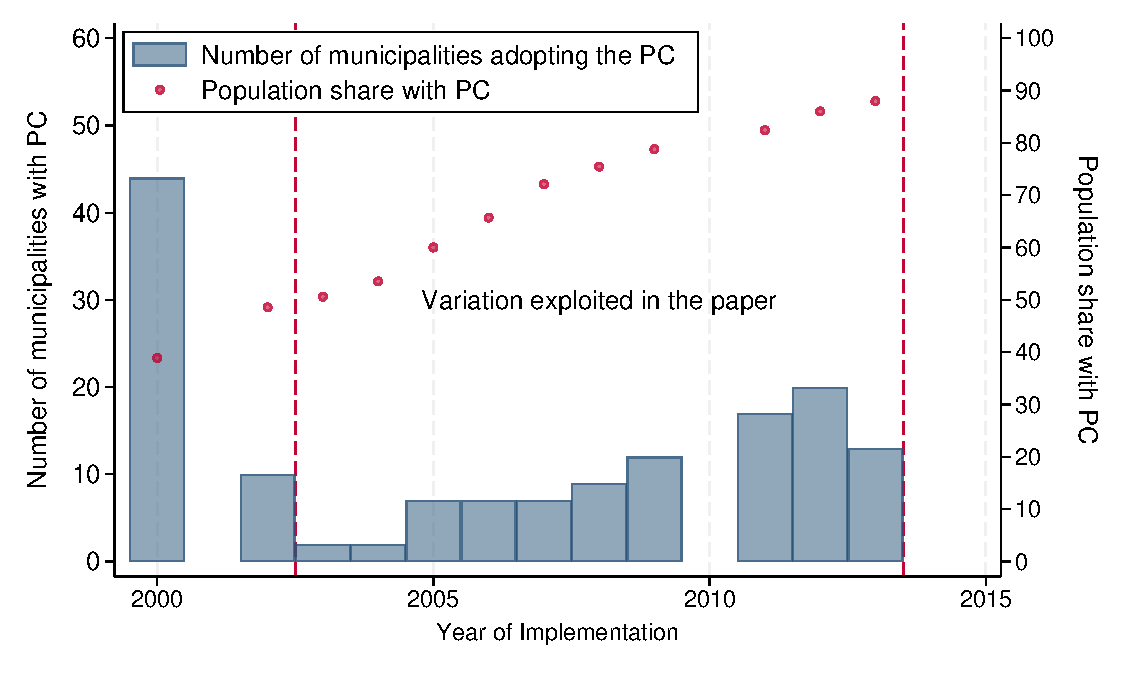
\includegraphics[width=1\textwidth]{../manuscript/Graphs/Graph_PCvariation.pdf}
        \caption{Adoption of \emph{Plan Cuadrante}}
    \end{subfigure}
    \\
    \begin{subfigure}{\textwidth}
    \centering
    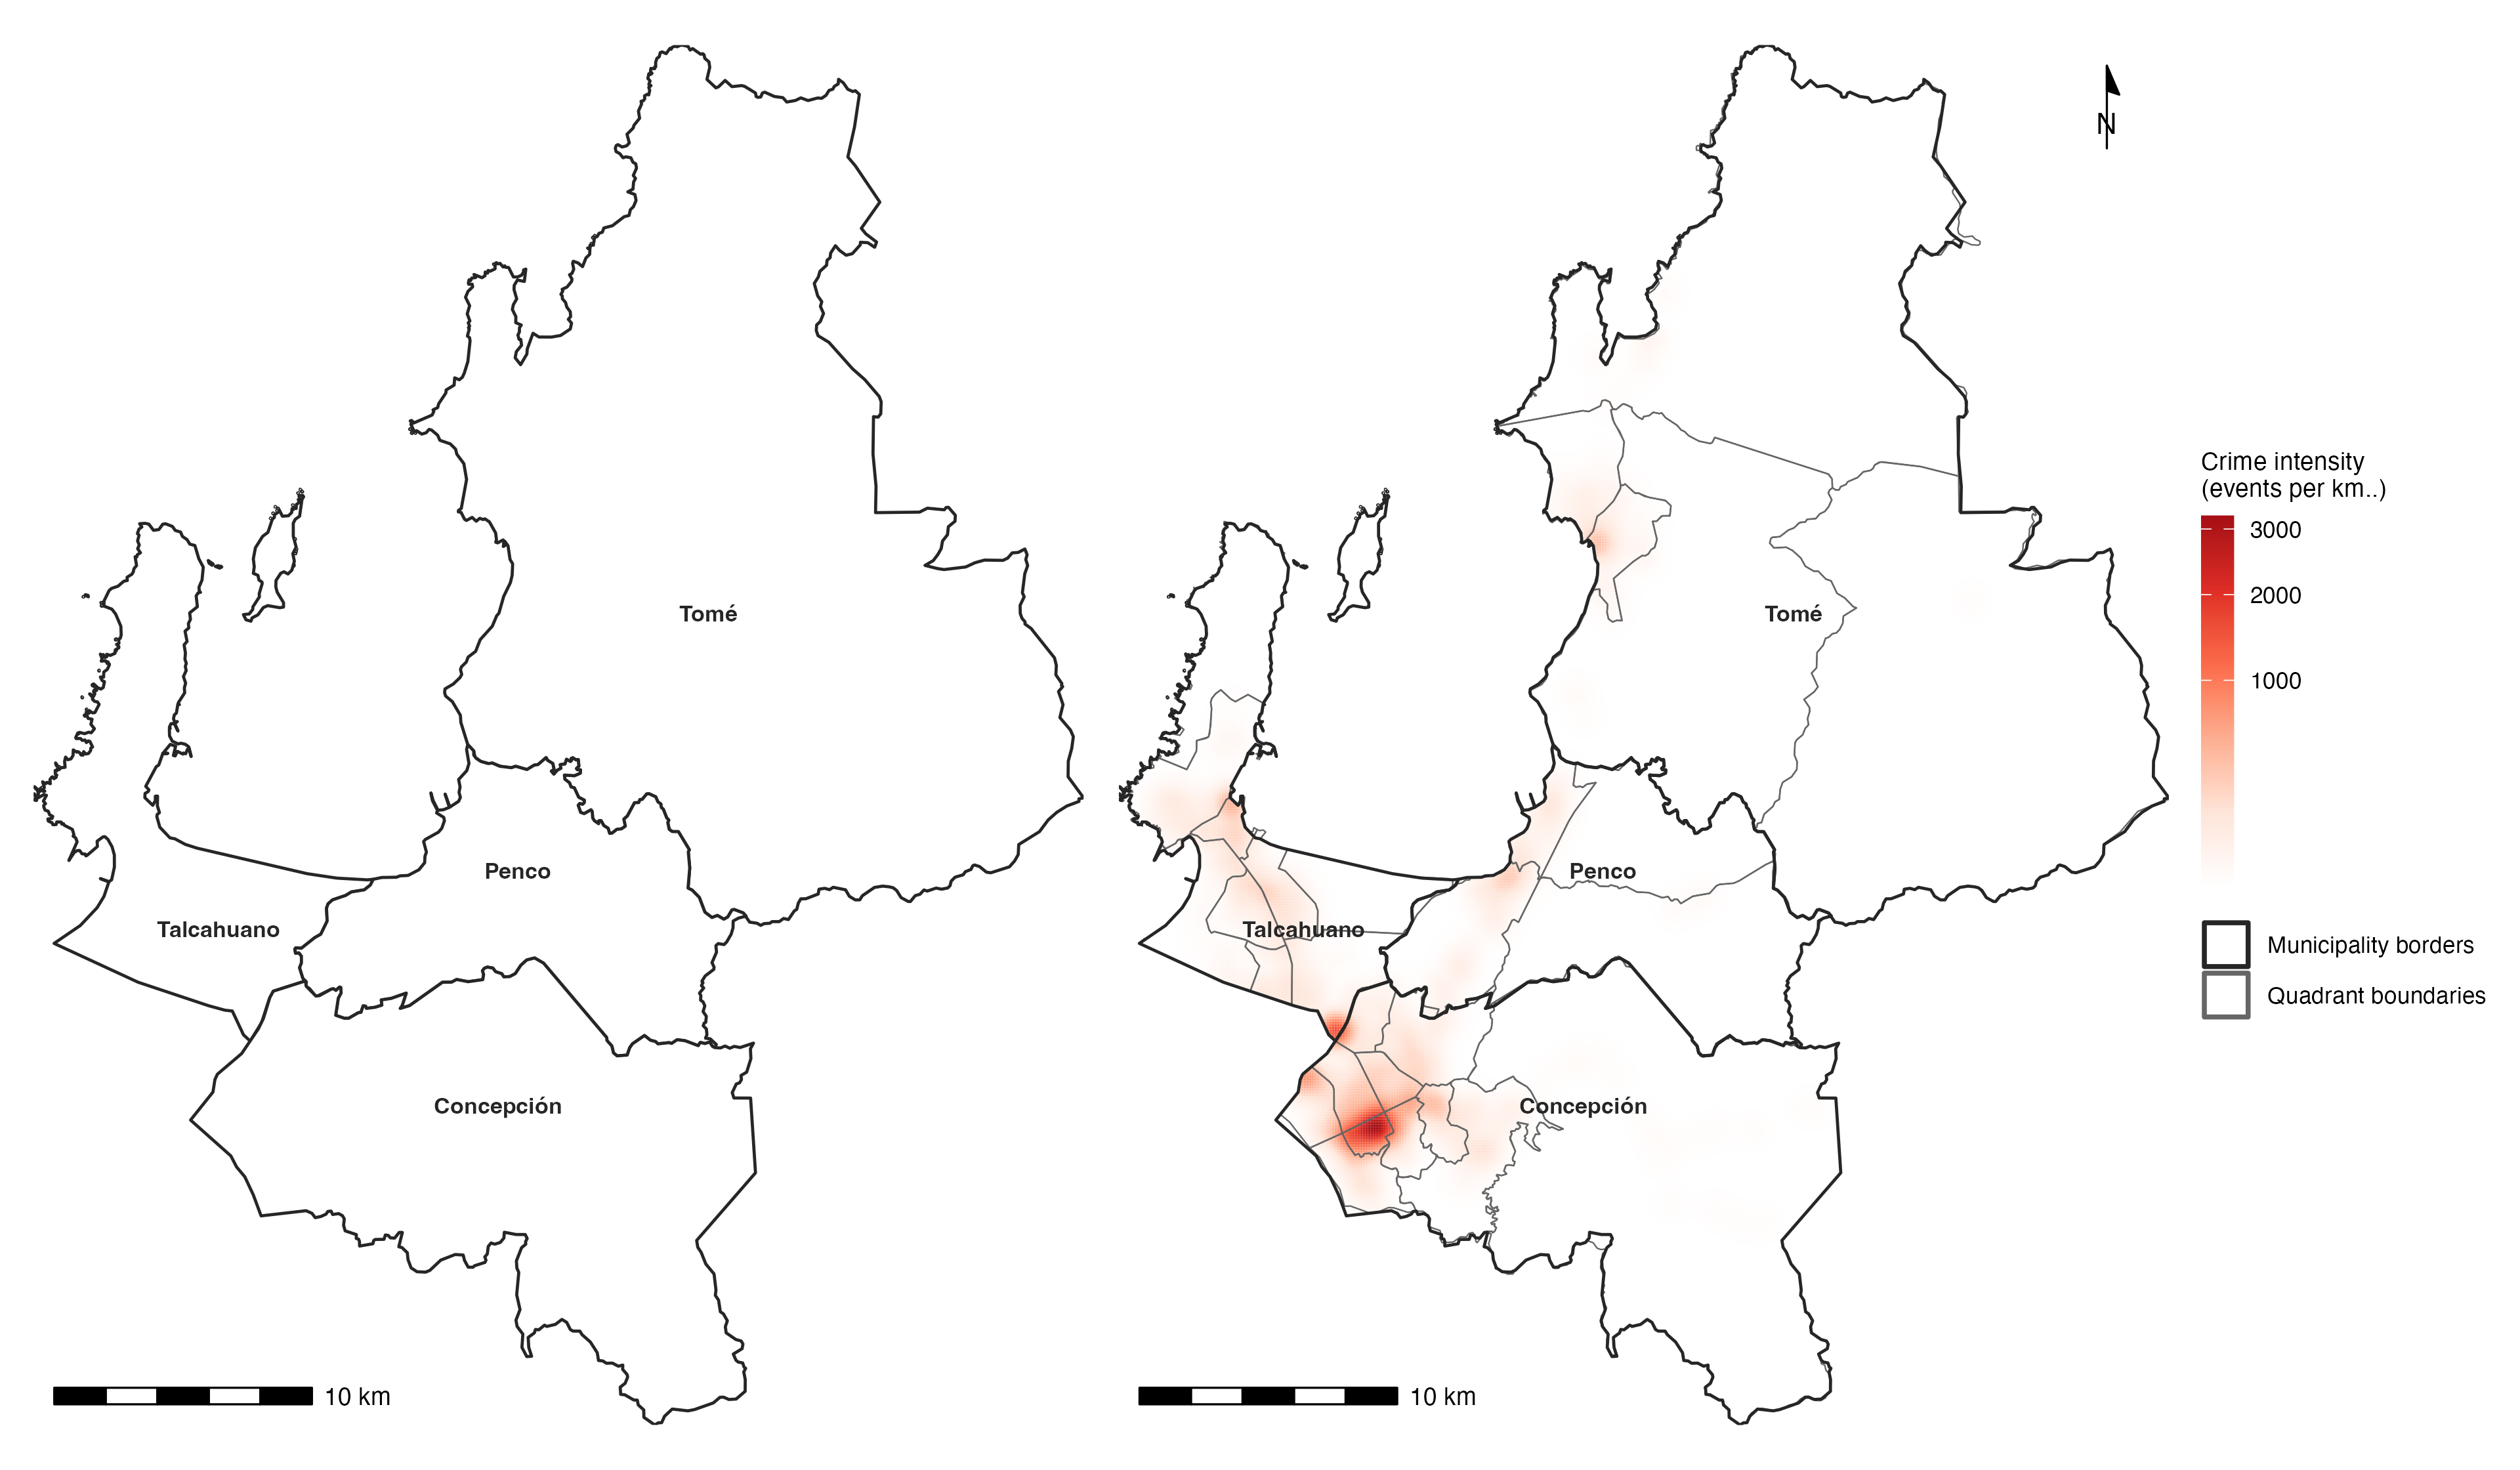
\includegraphics[width=0.65\linewidth]{../manuscript/Graphs/Graph_PCexample_combined.png}
    \caption{\emph{Plan Cuadrante} in the Concepci\'on area}
    \end{subfigure}%
 %   \\
 %   \begin{subfigure}{0.58\textwidth}
 %       \centering
 %       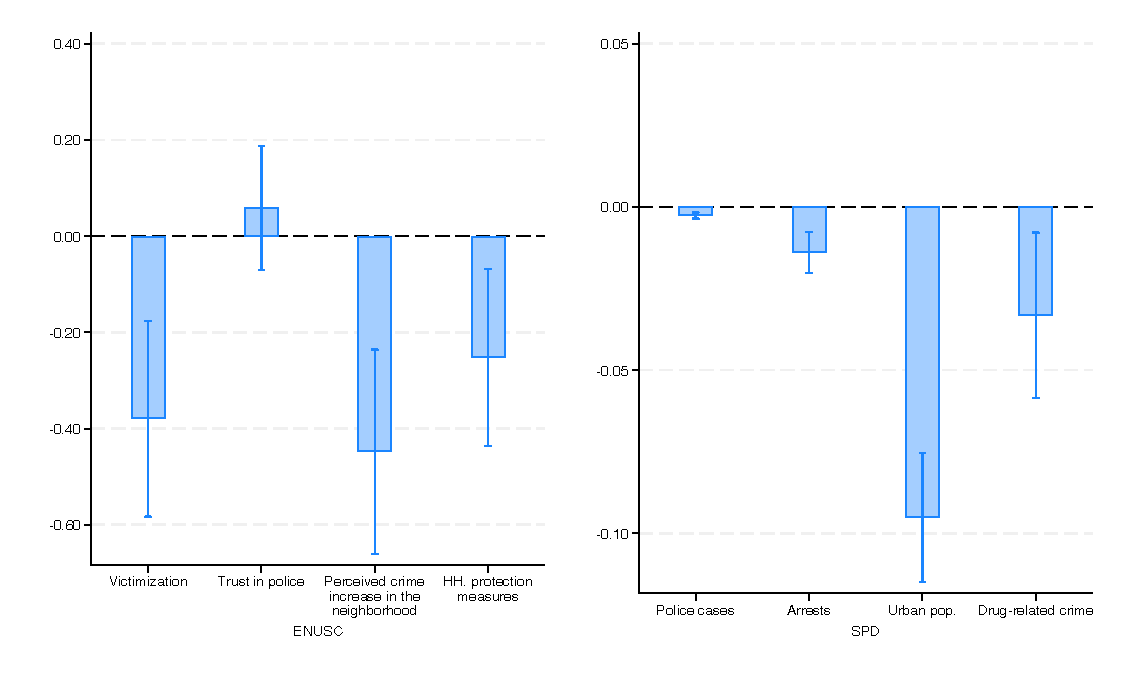
\includegraphics[width=1.1\textwidth]{../manuscript/Graphs/results_predictorsPC_combined.pdf}
 %       \caption{Time of Adoption and Municipality Characteristics}
  %  \end{subfigure}%
    \\[12pt]
    \begin{minipage}{0.95\textwidth}
    \footnotesize Notes: Panel (a) shows the number of municipalities adopting the \emph{Plan Cuadrante} each year (bars), while the circles above them illustrate the cumulative share of the Chilean population living in a municipality with the \emph{Plan Cuadrante} already in place. Panel (b) depicts the metropolitan area of Concepci\'on, the second-largest in Chile: the left map shows its four municipalities---the original police catchment areas---and the right map overlays the Carabineros quadrants together with a kernel-density estimate of all types of robberies and thefts recorded by the police (both reported crimes and arrests). It illustrates how \emph{Plan Cuadrante} subdivided each catchment area (which corresponds to the territory of a municipality) into smaller quadrants, as well as the spatial concentration of crime within them.
    \end{minipage}
\end{figure}
\clearpage

\FloatBarrier

Conceptually, police effectiveness can be viewed as a function of three inputs: total resources, territorial deployment, and policing strategy. Although in some municipalities police resources were increased significantly to operationalize the beat policing model \citep{DIPRES2007_largo,DIPRES2014}, the program primarily transformed the latter two elements. The creation of quadrants was accompanied by permanent geographic assignment of officers to specific areas. This change was operationally critical. By making officers responsible for their quadrant, it encouraged accumulation of local knowledge and stronger community ties, allowing them to adapt patrols and prevention activities to local crime patterns. Importantly, this was not driven by program-specific operational directive changes. Throughout the period we study, a single national set of operational guidelines applied to officers in both treated and control municipalities \citep{Manual_Carabineros2018,DIPRES2007_largo}. Thus, while the average effects we document on crime and crime perception likely reflect combined changes in the three elements we discuss---i.e., resources, deployment, and strategy---the deployment change itself was essential to operationalizing the reform. We discuss the drivers of the effects we document in Section \ref{mechanisms}.

Quadrant size and shape were determined by local police authorities based on factors such as road networks, geographic features, and available resources. In principle, resource allocation across quadrants followed demand for police services, measured in Equivalent Surveillance Units (UVEs); in practice, the station commander retained discretionary authority, as was also the case prior to \emph{Plan Cuadrante} \citep{DIPRES2014}. Municipalities implementing \emph{Plan Cuadrante} were subdivided into an average of seven quadrants, each typically staffed by approximately three officers per shift. On average, each quadrant covered 185 square kilometers and served 13,466 inhabitants. Panel (b) of Figure \ref{fig:figure01} illustrates this structure, showing the 29 quadrants created across the four municipalities of the Concepción metropolitan region---Chile's second-largest metropolitan area and the largest in our sample. Quadrants represented approximately 14\% of the original \emph{comisar\'ia} territory. Officers continued to operate from the same police station but were permanently assigned to a specific sub-area within its jurisdiction. While Carabineros' hierarchical structure limits frontline officer decision-making authority, each quadrant was assigned a Quadrant Delegate (\textit{Delegado de Cuadrante}), a non-commissioned officer, responsible for immediate operational decisions within the quadrant.

\emph{Plan Cuadrante} may affect public safety through two complementary channels: deterrence and police effectiveness, understood as the capacity to respond to and resolve crimes. The changes induced by \emph{Plan Cuadrante}---permanently assigning officers to well-defined neighborhoods and, in some municipalities, increasing available resources---can increase both police visibility and local knowledge. As officers repeatedly patrol the same area, they become familiar with its streets, residents, and routines, which can raise the perceived probability of identification and apprehension and reduce the expected returns to crime. At the same time, this deeper knowledge of local territory and communities can improve police response and case resolution once crimes occur. The reform therefore likely affects both dimensions. Consistent with this interpretation, in Section \ref{results} we document declines in victimization and in reported crime---patterns consistent with deterrence---together with increases in arrests, consistent with improved police effectiveness.

Although beat policing shares features with other policing approaches, such as hot-spot policing and community-based policing, which have been widely studied, it has distinctive features that make it worth studying as an independent approach. Hot-spot policing concentrates resources in high-crime areas and does not focus on building local knowledge and community ties. It is typically implemented through targeted interventions at specific locations rather than systematic territorial organization, and the same officers are not necessarily sent repeatedly to the same areas. Evidence on hot-spot policing is mixed, with some studies showing crime reductions in targeted areas but also potential displacement effects \citep{SR_1}. \emph{Plan Cuadrante}, by contrast, subdivided all urban municipalities into quadrants with permanent officer assignment. As Panel (b) of Figure \ref{fig:figure01} illustrates, some quadrants contained crime hot-spots, but many did not. The reform thus addressed entire urban territories rather than specific high-crime areas, potentially mitigating displacement effects associated with hot-spot policing.

Community-based policing emphasizes building relationships with residents and addressing underlying social issues, and typically involves active community participation in defining strategy and priorities---in some cases, even assuming surveillance and prevention responsibilities. While increasing trust in the police and strengthening community ties were among the declared goals of \emph{Plan Cuadrante}, and may have resulted from its territorial reorganization, the community was not formally involved in the provision of security.\footnote{The \emph{Plan Cuadrante}'s original design contemplated a formal community integration model (MICC) with a Community Affairs Office (\textit{Oficina de Asuntos Comunitarios}) and a dedicated officer in each police station. However, this model was not implemented during our study period. Independent program evaluations from the Budget Office document that these Community Affairs Offices did not exist and had no dedicated personnel, budget, or structured activities in the period we study \citep{DIPRES2007_largo,DIPRES2014}. The community integration model was piloted in four police stations during 2012--2013, none of which are in our analytical sample. Financing was then discontinued in early 2014 and only restored and expanded after our study period ends.}%
 %Similarly, Operations Offices (\textit{Oficina de Operaciones}) formally assigned crime analysis functions but relied on paper-based entry systems, lacking digital infrastructure, analysts, or centralized data systems throughout the study period \citep{DIPRES2014}. Both the community integration model and crime analysis function were substantively implemented only with \emph{Plan Cuadrante} 2.0 (2015--2017) \citep{Carabineros2018}, outside our study period.}

In recent decades, police departments worldwide have transitioned toward beat policing reforms \citep{NASEM2018,PCSP2014}, yet the effectiveness of this model has not been rigorously assessed. Although the beat policing approach introduced through \emph{Plan Cuadrante} shares features with programs previously studied in the economic literature, its distinctive characteristics---comprehensive territorial reorganization and systematic local officer specialization---make it a valuable case for studying how deployment and policing strategies not yet examined in the economics literature affect crime and crime perception.



\section{Data and Empirical Strategy}
\label{identification}
\subsection{Data}

We combine administrative and survey data from \emph{Carabineros}, the Undersecretary for Crime Prevention, and the National Institute of Statistics (INE). 

\emph{Carabineros} provided information on \emph{Plan Cuadrante} implementation, which we use to define treatment status across municipalities over time. The National Institute of Statistics granted access to the National Survey on Security and Crime (ENUSC), a repeated cross-section first conducted in 2003 and administered annually between October and December since 2005. The survey covers more than 25,000 households across 101 urban municipalities, collecting information on crime victimization, perceptions, trust in police, and household prevention measures over the previous 12 months.\footnote{The survey is administered to a randomly selected household member who must: a) live in the household, b) be 15 years or older, c) not be a domestic worker, and d) not have any disability preventing survey comprehension.}

Our empirical approach excludes always-treated municipalities \citep{Callaway}. Given ENUSC's first implementation in 2003 and absence in 2004, our main sample includes households from 46 urban municipalities that adopted \emph{Plan Cuadrante} between 2005 and 2012 plus one never-treated municipality.\footnote{This sample excludes municipalities adopting \emph{Plan Cuadrante} in 2013 as they are not covered by ENUSC. Also, there is only one never treated municipality covered by ENUSC.} The treated municipalities in this analytical sample account for approximately 27\% of Chile's population. 


The Undersecretary for Crime Prevention provided data on the number of reported crimes (2002--2016) and arrests (2005--2016) for all municipalities. This comprehensive coverage allows us to expand the analytical sample: for reported crime, we include all municipalities adopting \emph{Plan Cuadrante} after 2002 together with never-treated municipalities, for a total of 292 municipalities; for arrests, the corresponding sample includes all post-2005 adopters and never-treated municipalities, for a total of 281 municipalities. The treated municipalities in these analytical samples account for over half of Chile's population.


The study period differs across the two data sources, as each covers a different time span and a different set of municipalities. For the ENUSC-based analysis, it is restricted to 2003--2012. The \citet{Callaway} estimator uses not-yet-treated and never-treated municipalities as the comparison group. Since only one municipality in the survey sample is never treated, extending the analysis beyond 2012---the last year in which a municipality surveyed in ENUSC adopts the program---would leave only that single never-treated unit as the comparison group for subsequent periods, making the estimates unreliable. The administrative data, by contrast, cover a large number of never-treated municipalities that can serve as controls throughout the full data period, allowing us to exploit the complete administrative coverage---2002--2016 for reported crime and 2005--2016 for arrests---and to include all municipalities adopting the program from 2003 to 2013, when the last municipality joins \emph{Plan Cuadrante}.


Together, the treated municipalities in our two analytical samples represent substantial shares of the Chilean population---approximately 27\% in the ENUSC-based analysis and over half in the administrative data analysis---and are geographically distributed across the country rather than clustered in a single region. Tables \ref{tab:sum_statsA2} and \ref{tab:sum_statsA3} in Online Appendix \ref{sec:appendixA} and Table \ref{tab:comparing_samples} and Figure \ref{fig:pcsp_maps} in Online Appendix \ref{sec:appendixB} provide a detailed characterization of the treated municipalities in each analytical sample relative to the average Chilean municipality.

\subsection{Empirical Strategy}

To estimate \emph{Plan Cuadrante}'s effect on the outcomes of interest, we exploit its staggered adoption across Chilean municipalities between 2003 and 2013. Analyses relying on ENUSC data use variation from 2005-2012 adoptions, while those relying on administrative data use variation from 2003-2013 adoptions.\footnote{As a robustness check, we estimate effects on administrative data outcomes using only municipalities in the
ENUSC sample. Online Appendix Table \ref{tab:SPD_all_vs_enusc} and Figure \ref{fig:figure02_N47} show that the magnitude of these effects in the restricted sample is larger for reported crime but qualitatively similar
to the ones we present in Section \ref{results}.}

Treatment exposure is defined at the municipality-year level. ENUSC provides household-level repeated cross-sections with municipality identifiers, enabling household-level analysis for survey data. The administrative police records are available only at the municipality level, requiring aggregated analysis for reported crime and arrests. We estimate the following difference-in-differences specification:

\begin{equation}
Y_{imt}= \beta_0 + \beta_{1} \mbox{\textit{PC}}_{mt} +  \mu_{m}   +      \mu_{t} +  \varepsilon_{imt}
\label{eq:main}
\end{equation}

\noindent where $Y_{imt}$ is the outcome of interest reported by household $i$ from municipality $m$ in year $t$ or observed in administrative data for municipality $m$ in year $t$; $PC_{mt}$ indicates whether municipality $m$ had implemented \emph{Plan Cuadrante} by year $t$; $\mu_m$ and $\mu_t$ are municipality and year fixed effects; and $\varepsilon_{imt}$ is the error term. The parameter $\beta_{1}$ measures the program's effect on police effectiveness.

Given the staggered adoption of the program, standard two-way fixed-effects models could generate negative weights \citep{GoodmanBacon}. We address this concern using \citet{Callaway}'s estimation procedure for staggered treatment adoption with multiple periods. 
Online Appendix Figure \ref{fig:figureA2_alterestim} shows robustness to alternative estimators, including those developed by \citet{Chaisemartin, Gardner, wooldridge2023simple}, as well as to the canonical two-way fixed effects (TWFE) estimator. The resulting estimates are remarkably similar across the alternative staggered-adoption estimators, except for the canonical TWFE, which shows attenuated effects, arguably driven by the negative weights problem discussed above \citep{GoodmanBacon}. The corresponding event studies, reported in Online Appendix Figures \ref{fig:alterestim_delitos}, \ref{fig:alterestim_inseguridad}, \ref{fig:alterestim_medidas}, and \ref{fig:alterestim_crime}, confirm that pre-adoption trends are flat under each alternative estimator.

Our empirical approach accounts for time-invariant differences between early- and late-adopting municipalities, as well as time-specific shocks that affect municipalities with and without \emph{Plan Cuadrante} similarly. The key identification assumption is that, in the absence of \emph{Plan Cuadrante}, the outcomes of interest would have followed parallel trends. While we cannot
formally test this assumption, we present dynamic specifications that confirm parallel pre-adoption trends across the municipalities in our sample. 

An additional threat to the causal interpretation of our estimates is potential spillovers, either through crime displacement from treated to control municipalities or through police resource reallocation from control to treated municipalities. We probe this concern directly in Section \ref{sec:spillovers}, where a battery of spillover tests consistently finds no evidence of such effects. Online Appendix \ref{sec:appendixC} presents a variety of additional robustness checks that show that our results are robust to the use of different estimation samples and of different crime perception measures, and reports a placebo exercise that confirms the absence of effects on crimes that we would not expect to respond to \emph{Plan Cuadrante}.

Finally, for statistical inference, we cluster standard errors at the municipality level. Since we work with a relatively small number of large clusters, we compute standard errors using wild bootstrapping \citep{Cameron}.

\section{Results}
\label{results}
This section presents the main results of the paper. First, it shows that \emph{Plan Cuadrante} significantly improved crime and crime perception outcomes. Second, it shows that these effects were consistent across municipalities with different population densities and with varying socioeconomic levels. Finally, the section studies which components of the program are driving the effects. 

\subsection{Effects of \emph{Plan Cuadrante} on Crime and Security Perception}
\label{main_results}

Panels (a) to (d) in Figure \ref{fig:figure02} present estimates of the dynamic effects of \emph{Plan Cuadrante} on victimization, reported crime, crime perception, and investment in household security measures. The blue circles and bars represent pre-adoption estimates and their 95\% confidence intervals. Very few of these pre-treatment coefficients are statistically significant, and the average pre-treatment effects are overall reassuring,\footnote{The p-values for the test that the average pre-treatment effect equals zero are 0.833 for victimization, 0.204 for reported crime, 0.178 for security perception, and 0.066 for the adoption of security measures.} suggesting that the outcomes that we study followed parallel trends before the program's introduction.%The p-values for the \emph{joint} significance test of the pre-treatment coefficients are, respectively, 0.101, 0.049, 0.076, and 0.109. The only marginal case is the joint test for reported crime, where the pre-treatment coefficients are slightly positive and therefore conservative with respect to the negative effect we estimate.0.159 for arrests, 0.300 for trust in police 
 

\FloatBarrier
%--- Implementation
\begin{figure}[h!]
    \centering
    \caption{Effects of \emph{Plan Cuadrante} on Crime Outcomes and Security Perceptions}
    \label{fig:figure02}
    \begin{subfigure}{0.495\textwidth}
        \centering
        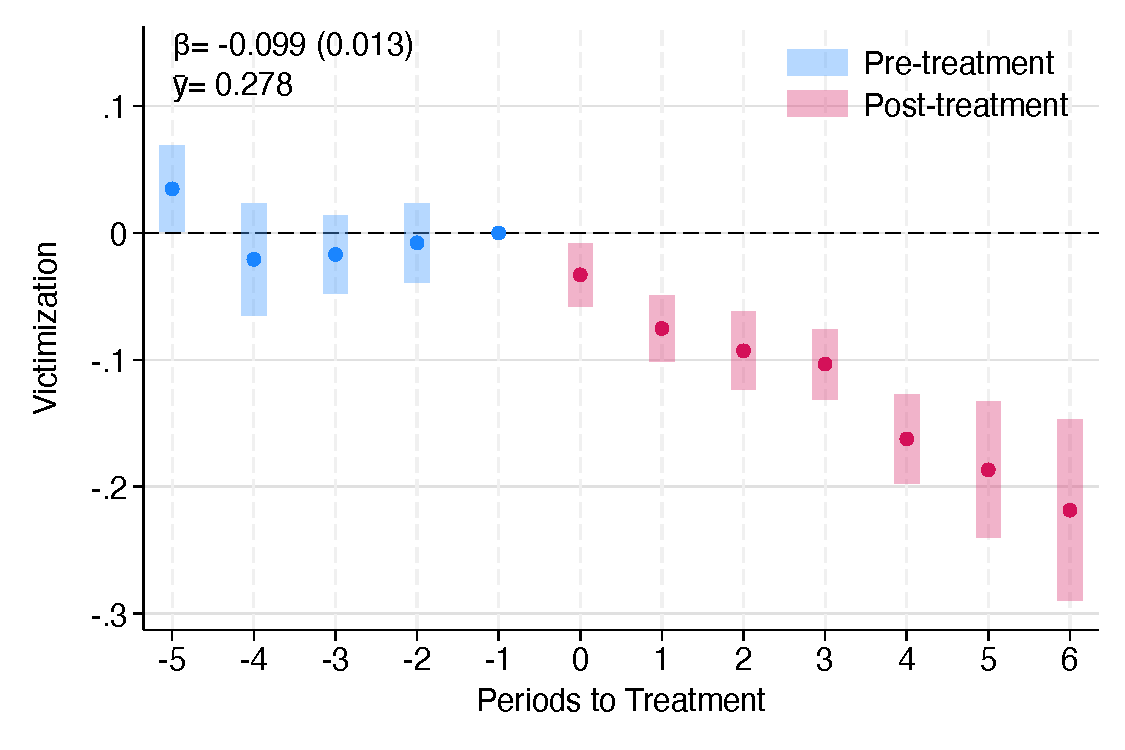
\includegraphics[width=\textwidth]{../manuscript/Graphs/results_victimization.pdf}
        \caption{Victimization in last 12 months}
    \end{subfigure}%
    ~
    \begin{subfigure}{0.495\textwidth}
    \centering
    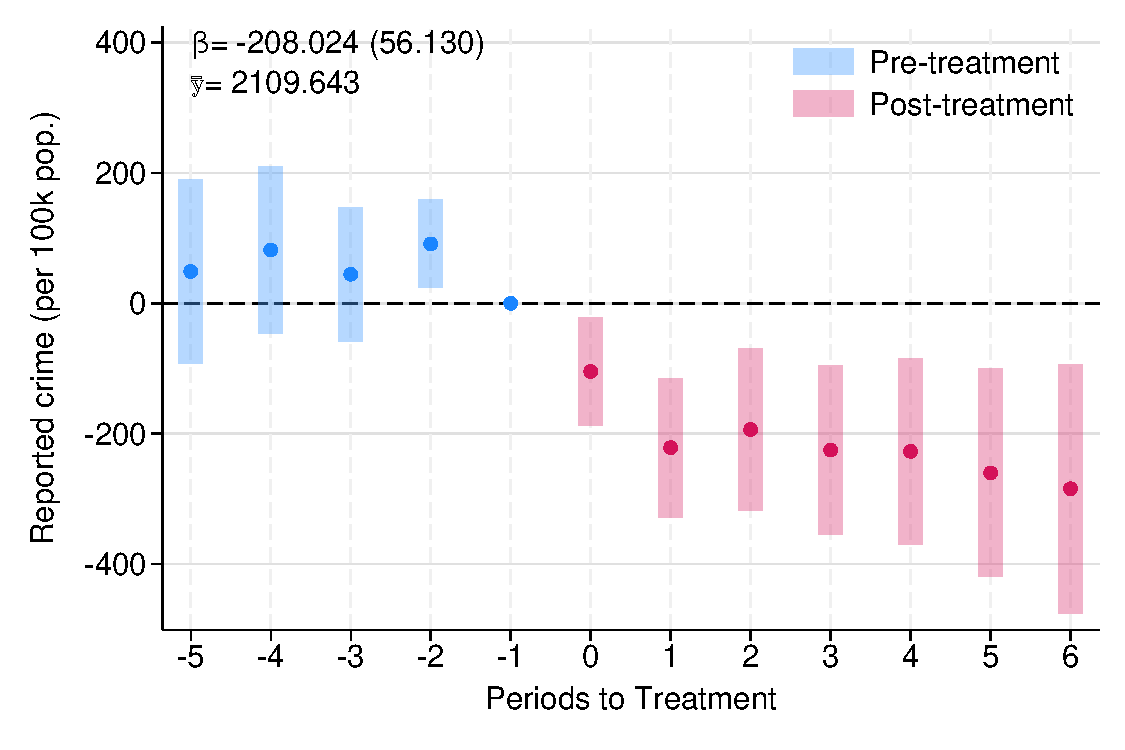
\includegraphics[width=\textwidth]{../manuscript/Graphs/totalreportedcrime_allcomunas.pdf}
        \caption{Reported crime per 100k inhabitants}
    \end{subfigure}
        \begin{subfigure}{0.495\textwidth}
        \centering
        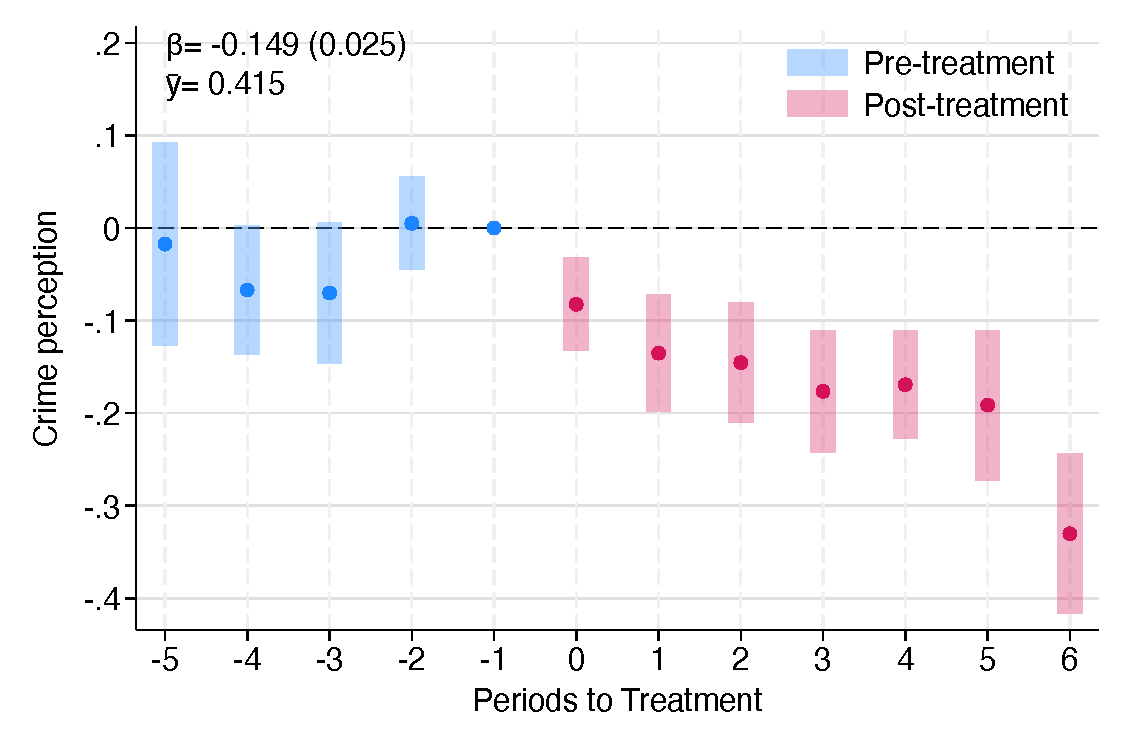
\includegraphics[width=\textwidth]{../manuscript/Graphs/results_perception.pdf}
        \caption{Households reporting an increase in crime}
    \end{subfigure}%
    ~
    \begin{subfigure}{0.495\textwidth}
    \centering
    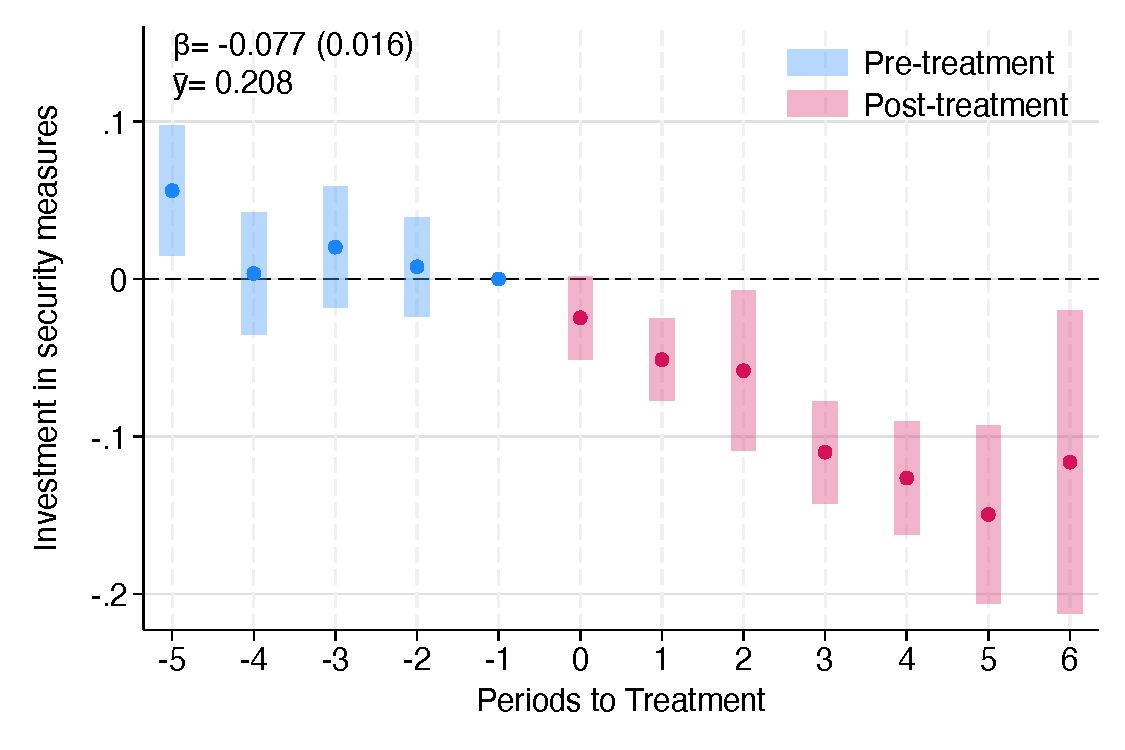
\includegraphics[width=\textwidth]{../manuscript/Graphs/results_hhprotectionmeasures.pdf}
        \caption{Households adopting security measures}
    \end{subfigure}
    \\[12pt]
    \begin{minipage}{0.99\textwidth}
    \footnotesize
    Notes: This figure shows the dynamic effects of the \emph{Plan Cuadrante} on different measures of police effectiveness. The estimation is conducted using the procedure developed in \citet{Callaway} for difference-in-differences with staggered treatment adoption. The dots in the figure represent the estimated coefficients and the bars behind them 95\% confidence intervals. Standard errors are clustered at the municipality level using the wild bootstrapping procedure. The pooled effect and the mean outcome before the introduction of the treatment is also presented in each panel. Panel (a) reports the effect of \emph{Plan Cuadrante} on the probability of household victimization in the last 12 months using the ENUSC survey. Panel (b) reports the effect on the number of crimes reported to the police in the municipality per 100,000 inhabitants using administrative data. Panel (c) reports the effect on the probability of perceiving an increase in crime using the ENUSC survey. Panel (d) reports the effect on the probability of adopting security measures in the last twelve months using the ENUSC survey. Panel (a) includes 93,041 observations; panel (b), 4,231; panel (c), 89,578; and panel (d), 93,041 observations.
    \end{minipage}
\end{figure}

\FloatBarrier

The red circles and bars represent post-adoption estimates and illustrate the program's effects.\footnote{The analyses we present in this section come from an unbalanced panel of municipalities. Thus, each lead and lag is identified using a different subset of municipalities. Online Appendix Figure \ref{fig:figureA6_bp} replicates these analyses using only municipalities that implemented \emph{Plan Cuadrante} between 2006 and 2009, allowing us to build a balanced panel between t-2 and t+3. The estimates remain remarkably similar.}

Panel (a) shows that after adopting \emph{Plan Cuadrante}, there was a significant drop in the share of households reporting crimes in the previous 12 months. This decline in victimization begins in the adoption year and continues over time, falling by ten percentage points (36\%) on average. Consistently, panel (b) shows a substantial decrease in reported crimes. Expressed per hundred thousand inhabitants to normalize across municipality sizes, we find an average reduction of 208 reported crimes (10\%) following the adoption of the program.\footnote{Table \ref{tab:bonferroni} in Online Appendix \ref{sec:appendixC} applies the Bonferroni correction across the main outcome estimates and confirms that these results are not a product of multiple hypothesis testing.}\footnote{For symmetry with the ENUSC-based analysis, this event study is restricted to 5 pre-treatment and 7 post-treatment periods. Since the administrative data cover a much larger number of never-treated municipalities than the ENUSC sample, we can estimate this effect over a longer window of pre-treatment and post-treatment periods; Online Appendix Figure \ref{fig:admin_uncapped} reports the results for reported crime and arrests using the full set of post-treatment and pre-treatment periods, which are very similar to those presented here.}\footnote{Online Appendix Figure \ref{fig:figureA9} reports a placebo exercise confirming the absence of effects on crimes that we would not expect to respond to \emph{Plan Cuadrante}.}\footnote{As a further robustness check, we implement a placebo/randomization-inference exercise in which adoption dates and never-treated status are randomly reassigned 1,000 times: our estimated direct effect on treated municipalities falls in the bottom first percentile of the resulting placebo distribution, while the analogous estimate for untreated neighbors of treated municipalities falls near its center---consistent with a genuine effect on treated municipalities and with the absence of spillovers documented in Section \ref{sec:spillovers} (Online Appendix \ref{sec:ri_appendix}).} Note, however, that analyses based on reported cases may underestimate the reform's true impact since not all crimes are reported to the police.\footnote{Online Appendix Figure \ref{fig:figureA8} replicates the analyses in panels (a) and (b) by crime type, showing significant reductions in both property and violent crimes. While the definitions of crime categories differ across survey and administrative data, the program's effects are consistent in magnitude and statistical significance for violent theft, assault, and home burglary in both datasets.}
%, and improved trust in police could increase reporting rates, making any observed reductions in reported crime a conservative estimate of the actual crime decline.
%Panel (c) shows that despite the decrease in victimization and reported crime, arrests per hundred thousand inhabitants increased following the adoption of \emph{Plan Cuadrante}. This simultaneous decrease in crimes and increase in arrests suggests improved police effectiveness.

The results above show that \emph{Plan Cuadrante} reduced both victimization and reported crime. But did this change in public safety translate into increased security perception? Panel (c) reveals that \emph{Plan Cuadrante} decreased insecurity perception, with households reporting increased neighborhood crime dropping by 15 percentage points (36\%).\footnote{Online Appendix Figure \ref{fig:figureA3} reports similar declines in insecurity perception measured at the municipality and country levels.} In line with this result, panel (d) shows that following the program implementation, households adopting protective measures---such as buying dogs or weapons, installing alarms or fences, and purchasing insurance or private security---decreased by eight percentage points (37\%).\footnote{Online Appendix Table \ref{tab:hhprotectionmeasurestype} disaggregates this analysis by measure type.}
%Panel (d) shows that households reporting high or very high trust in police increased by 12 percentage points (30\%) in adopting municipalities. 

In sum, \emph{Plan Cuadrante} reduced both criminal activity and security perception, while also decreasing private investment in security measures.\footnote{These results are robust to excluding municipalities most affected by the 2010 Maule earthquake, defined as those with a Modified Mercalli Intensity greater than 7; see Figure \ref{fig:figure02_noEQ} in Online Appendix \ref{sec:appendixC} for details.}

%To benchmark the scale of these effects in more intuitive terms, we translate the estimated decline in victimization into the number of victims avoided. Using the average annual cost of the program per municipality---US\$3.47 million \citep{DIPRES2007_largo, DIPRES2014}---and the 2017 Census total population across the 150 municipalities that adopted \emph{Plan Cuadrante}---15,424,263 inhabitants \citep{INE2017_censo}---the implied cost per victim avoided is about US\$338. Because beat policing is essentially a reorganization of police deployment, municipalities or police departments that are already well staffed and equipped would face substantially lower implementation costs. Overall, the cost of \emph{Plan Cuadrante} compares favorably with the substantial social and economic costs that crime imposes on households and communities in Latin America \citep{jaitman2017costs}.


%each percentage-point increase in trust in the police costs approximately US\$289,000, and  and each additional arrest per 100,000 inhabitants approximately US\$72,000

\subsection{\emph{Plan Cuadrante} and Spatial Spillovers}
\label{sec:spillovers}
%\textbf{4.2 \emph{Plan Cuadrante} and Spatial Spillovers}

Beyond parallel trends, a causal interpretation of our estimates requires the absence of spillover effects from treated to control municipalities, since such spillovers could bias treatment effects upward. This concern is relevant in our setting. Previous work on deployment-based policing reforms, such as hot-spot policing, shows that crime may be displaced to nearby areas \citep{Blattman_Tobon_JEEA}. Spillovers could also arise through the reallocation of police resources from control to treated municipalities.

In our setting, spillovers are less likely for several reasons. First, as discussed in Section \ref{institutions}, \emph{Plan Cuadrante} introduced beat policing in Chile by reorganizing deployment across the full municipal territory rather than concentrating resources in specific hot spots. Second, Chilean municipalities are large---on average 101,000 inhabitants and 2,000 square kilometers \citep{SINIM}---and criminals typically do not travel such long distances to commit crimes, which makes displacement to other municipalities unlikely \citep{Langella}. Third, and more directly related to police resources, police regulations assign officers to \emph{comisar\'ias}---broader operational units that usually cover an entire municipality---for fixed periods, which limits rapid reallocation of officers across jurisdictions.\footnote{See the Transfer Manual for Carabineros de Chile Personnel available at \url{https://www.carabineros.cl/transparencia/og/pdf/OG_2707_13112019.pdf}}

We nonetheless assess spillovers empirically through two complementary exercises using administrative data at the national level. Online Appendix \ref{sec:appendixC} reports the full results. First, following \citet{crepon2013}, we test whether higher exposure to \emph{Plan Cuadrante} among neighboring municipalities affects outcomes in control municipalities. Online Appendix Figures \ref{fig:figure_continuous_spillovers} and \ref{fig:figure_count_spillovers}---which define neighbor exposure as the share and the number of treated neighbors, respectively---show no meaningful effects across the outcomes we study, suggesting the absence of spatial spillovers. Because exposure to treated neighbors is not randomly assigned, however, this evidence does not fully rule out the possibility that municipalities with many early-adopting neighbors differ systematically from those with fewer such neighbors in other respects that are also correlated with our outcomes.

Second, we estimate the effect of \emph{Plan Cuadrante} on police-reported crime and police resources in untreated municipalities whose neighbors adopt the program. Online Appendix Figure \ref{fig:spillover_admin} summarizes these estimates and again shows no evidence of spatial spillovers.

The exercises above evaluate spatial spillovers using administrative records for the extended municipality sample. We complement this evidence with two additional analyses focused on ENUSC municipalities. First, we re-estimate the administrative-outcome spillover analysis---for reported crime, arrests, police officers, and patrol vehicles---restricting the sample to neighbors of the 46 ENUSC municipalities (Online Appendix Figure \ref{fig:figure_46ENUSC_spillovers_admin}). Second, we test for spillovers directly in ENUSC outcomes. Because ENUSC coverage is limited---46 treated municipalities and 1 never-treated municipality, with only 10 sharing a border and 6 of those treated in different years---we estimate spillover effects from early-adopting ENUSC municipalities onto late-adopting ENUSC neighbors before the latter adopt the program (Online Appendix Figure \ref{fig:figure_results_spillovers_enusc}). Both exercises yield reassuringly null effects.

Taken together, these results indicate that spatial spillovers are unlikely to threaten identification in our setting.

\FloatBarrier

\subsection{Heterogeneous Effects of \emph{Plan Cuadrante} by Municipality and Households Characteristics}
\label{heterogeneity}

This section examines whether \emph{Plan Cuadrante}'s effects vary by population density, municipal poverty rates, and household socioeconomic status.\footnote{Data on population density and municipal poverty rates are available at \url{https://www.sinim.gov.cl/}} These analyses inform both external validity and distributional effects of the program. Figure \ref{fig:figure04_het} summarizes these results. We compare municipalities with low versus high population density, municipalities with low versus high poverty rates, and households with low versus high socioeconomic status by splitting the sample in two and estimating specification (\ref{eq:main}) independently in each subsample. For each split, we study four outcomes: victimization, reported crime, crime perception, and investment in security measures. Panels (a) and (b) plot victimization, crime perception, and investment in security measures---from the National Survey on Security and Crime (ENUSC)---on the left axis, and reported crime---from the administrative data of the Undersecretary for Crime Prevention---on the right axis. Because socioeconomic status is only observed in the ENUSC, panel (c) reports the three survey-based outcomes only. Blue and red bars represent $\beta_1$ estimates from different subsamples.

\FloatBarrier
%--- Implementation
\begin{figure}[h!]
    \centering
    \caption{Effects of \emph{Plan Cuadrante} by Population Density, Poverty, and Socioeconomic Status}
    \label{fig:figure04_het}
    \begin{subfigure}[t]{0.49\textwidth}
        \centering
        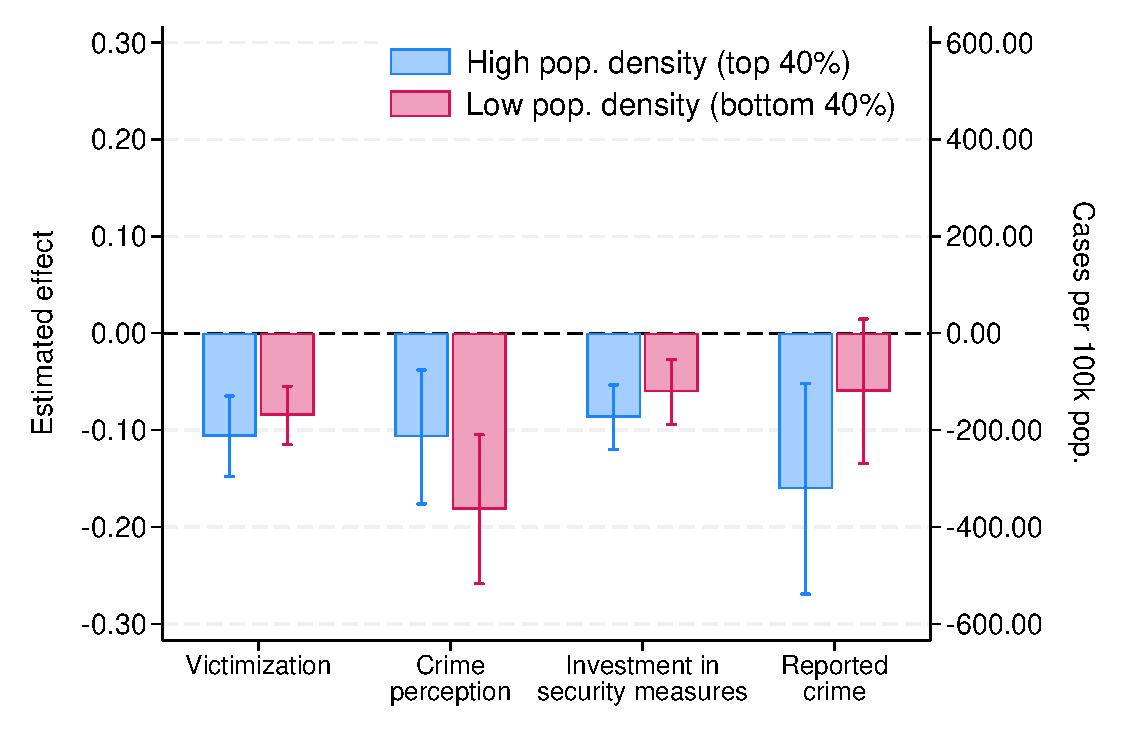
\includegraphics[width=\linewidth]{../manuscript/Graphs/results_het_density.pdf}
        \caption{By population density}
    \end{subfigure}\hfill
    \begin{subfigure}[t]{0.49\textwidth}
        \centering
        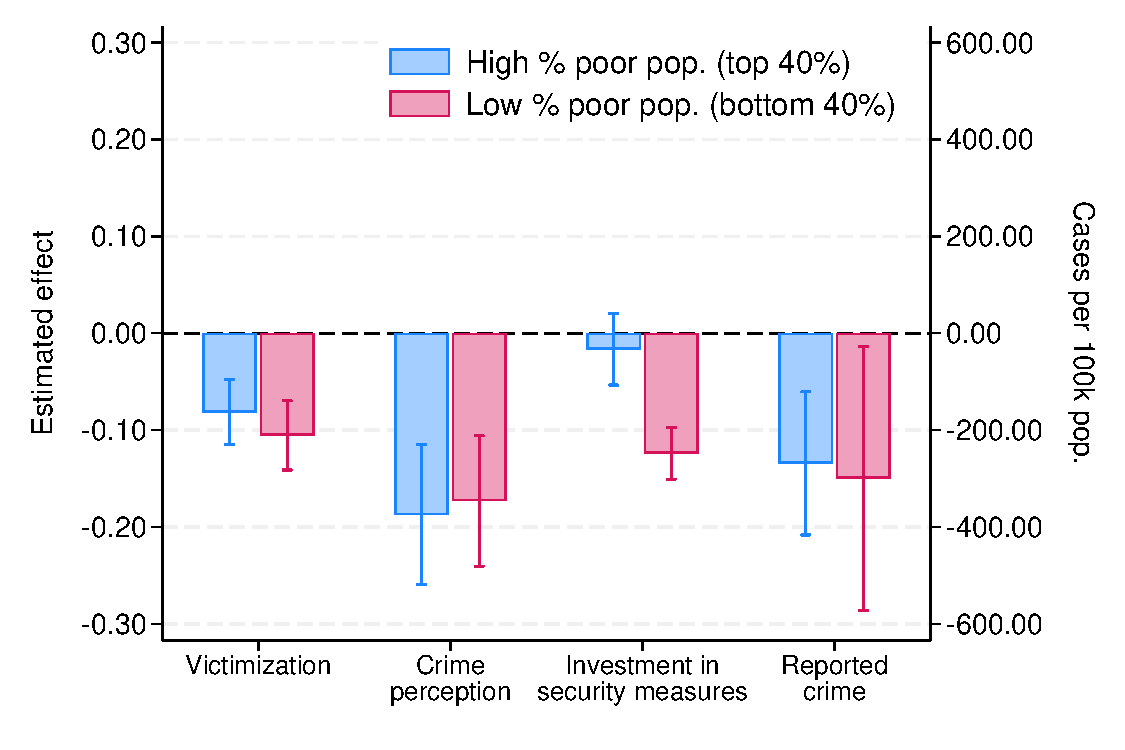
\includegraphics[width=\linewidth]{../manuscript/Graphs/results_het_poorpop.pdf}
        \caption{By population below poverty line}
    \end{subfigure}
    \\[8pt]
    \begin{subfigure}[t]{0.49\textwidth}
        \centering
        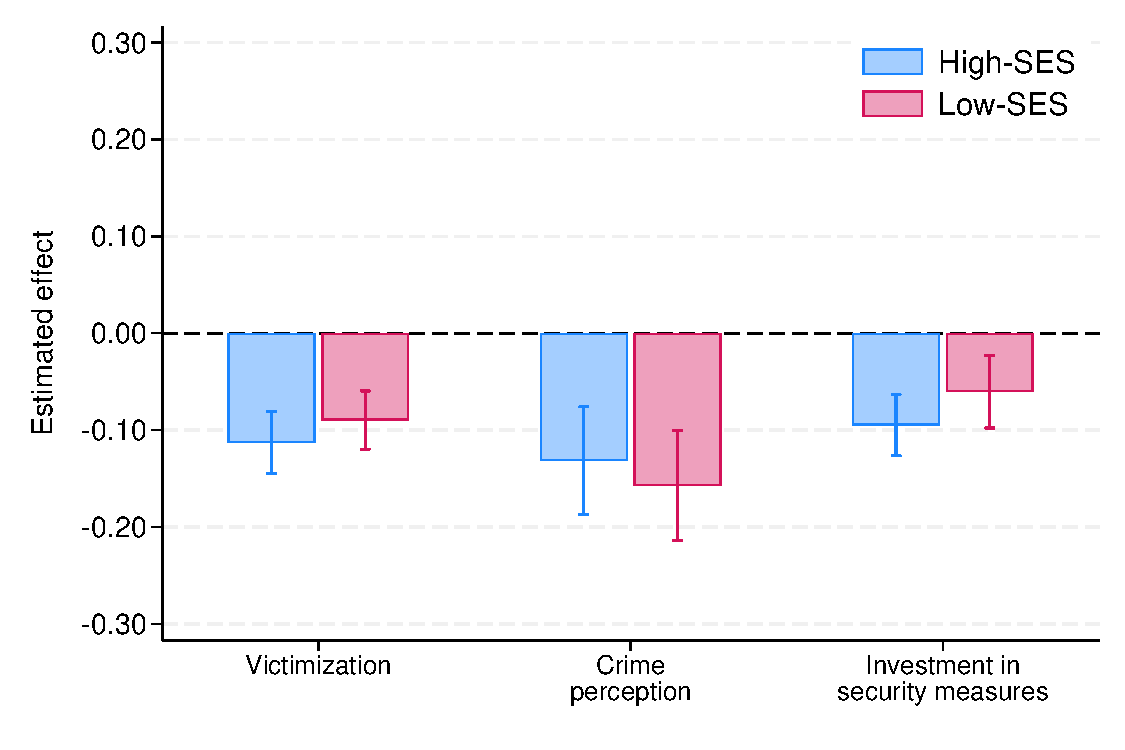
\includegraphics[width=\linewidth]{../manuscript/Graphs/results_het_SES.pdf}
        \caption{By household socioeconomic status}
    \end{subfigure}
    \\[10pt]
    \begin{minipage}{0.99\textwidth}
    \footnotesize Notes: This figure reports the heterogeneous effects of \emph{Plan Cuadrante} by population density (panel a), the proportion of poor people in the municipality (panel b), and household socioeconomic status (panel c). Each panel reports the effect on victimization, defined as the probability of household victimization in the last 12 months; crime perception, defined as the probability of perceiving an increase in crime; investment in security measures, defined as the probability of adopting security measures in the last twelve months; and reported crime, defined as the number of crimes reported to the police in the municipality per 100,000 inhabitants. Reported crime (administrative data, in cases per 100,000 inhabitants) is read on the right axis; all other outcomes, from the ENUSC survey (victimization, crime perception, and investment in security measures), are read on the left axis. Household socioeconomic status is only observed in the ENUSC, so panel (c) does not include reported crime. In panels (a) and (b), the bars compare municipalities in the two bottom quintiles (bottom 40\%) and in the two top quintiles (top 40\%) of the population density and poverty distributions, respectively. The average population density is 458 inhabitants per square kilometer in high-density municipalities and 29 in low-density municipalities; the average poverty rate is 28\% in high-poverty municipalities and 14\% in low-poverty municipalities. In panel (c), low-SES households include lower-class and lower-middle-class households, while high-SES households include upper-middle and upper-class households. The estimation is conducted using the difference-in-differences estimator for staggered treatment adoption developed in \citet{Callaway}. The graphs display the estimated coefficients and 95\% confidence intervals. Standard errors are clustered at the municipality level using the wild bootstrapping procedure.
    \end{minipage}
\end{figure}

\FloatBarrier

While \emph{Plan Cuadrante} was implemented only in urban municipalities, these areas vary substantially in size and structure. Yet panel (a) shows similar effects across population densities. Blue bars illustrate effects in high-density municipalities---top 40\% of density distribution---and red bars in low-density municipalities---bottom 40\%.\footnote{Average density: 458 inhabitants per square kilometer in high-density municipalities versus 29 in low-density municipalities.}

Panel (b) presents the results of a similar exercise comparing municipalities with different poverty rates. As in the case of population density, effects of \emph{Plan Cuadrante} seem to be similar across municipalities with high- and low-poverty rates. Blue bars show effects in high-poverty municipalities---top 40\% of poverty rate distribution---and red bars in low-poverty municipalities---bottom 40\%.\footnote{Average poverty rate: 28\% in high-poverty municipalities versus 14\% in low-poverty municipalities.}

Finally, panel (c) indicates that effects on victimization and security perception do not vary across household socioeconomic status (SES), based on ENUSC's household self-reported classification.\footnote{SES classification: Low-SES includes lower-class and lower-middle-class households; high-SES includes upper-middle and upper-class households.} Blue bars represent high-SES households, red bars low-SES households.

These results indicate that the beat policing model induced by \emph{Plan Cuadrante} benefited municipalities and households similarly, regardless of population density or socioeconomic status.

%% DANI, las figuras de heterogeneidad tienen que enfocarse exclusivamente en los outcomes de victimización, reported crime, percepción de inseguriad y adopción de medidas de seguridad. No hemos introducido los resultados de confianza en la policía y arrestos aún, por lo que sería raro que aparezcan acá.

\subsection{What Is Driving the Effects of \emph{Plan Cuadrante}?}%
\label{mechanisms}
%\textbf{4.4 What Is Driving the Effects of \emph{Plan Cuadrante}?}


To reduce crime and improve security perceptions, police forces need to strengthen both prevention and police effectiveness. Both margins can be shaped by resources, territorial deployment, and policing strategy. This section examines which components of \emph{Plan Cuadrante} are most likely to drive the effects documented in Section \ref{results}. 

The central objective of \emph{Plan Cuadrante} was to introduce a beat policing model by reorganizing deployment. Police operational territories that had typically matched municipal boundaries were subdivided into quadrants, and officers were permanently assigned to these quadrants. During our study period, national operational guidelines remained the same in adopting and non-adopting municipalities. Still, this new deployment likely affected policing strategy at a more operational level, because it allowed officers to adapt patrol routes, schedules, and prevention practices using the local knowledge that the program sought to build.

Although changes in resources were not the core of the reform, implementation contemplated increases in municipalities that lacked the personnel and patrol capacity required to move to this model. During the period we study, Chile was expanding public spending on security, and police resources increased in most municipalities regardless of whether or when they adopted \emph{Plan Cuadrante}. On average, however, municipalities adopting the program experienced larger increases in officers and patrol vehicles, as shown in panels (a) and (b) of Figure \ref{fig:resources}. Since increases in police resources have been shown to reduce crime in some contexts \citep{Evans}, this pattern raises a central question for interpretation, namely whether our estimates reflect resource expansion or the deployment and strategy changes introduced by \emph{Plan Cuadrante}. We address this question through a set of exercises that exploit heterogeneity in resource increases across municipalities and over time.

\FloatBarrier
%--- Implementation
\begin{figure}[H]
    \centering
    \caption{Plan Cuadrante and Changes in Police Resources}
    \label{fig:resources}
    \label{fig:figure_resources}
    \begin{tabular}{cc}
        \begin{minipage}[t]{0.48\textwidth}
            \centering
            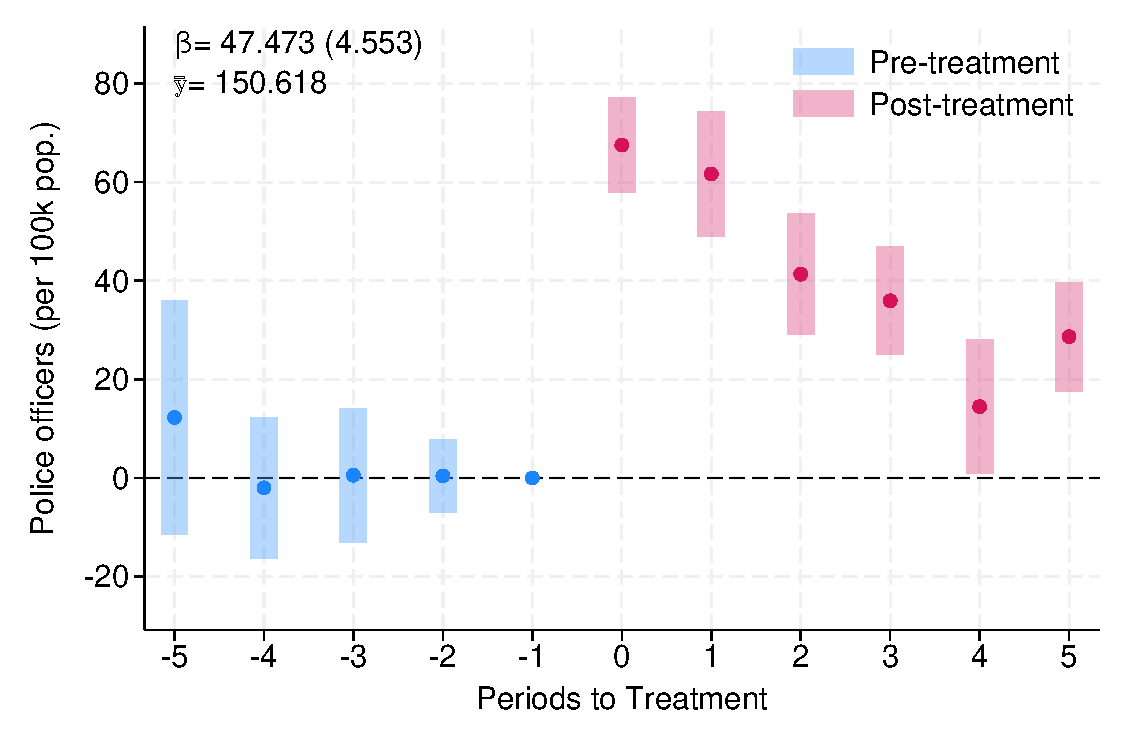
\includegraphics[width=\linewidth]{../manuscript/Graphs/fig4_officers.pdf}

            \small (a) Effect on the number of police officers
        \end{minipage}
        &
        \begin{minipage}[t]{0.48\textwidth}
            \centering
            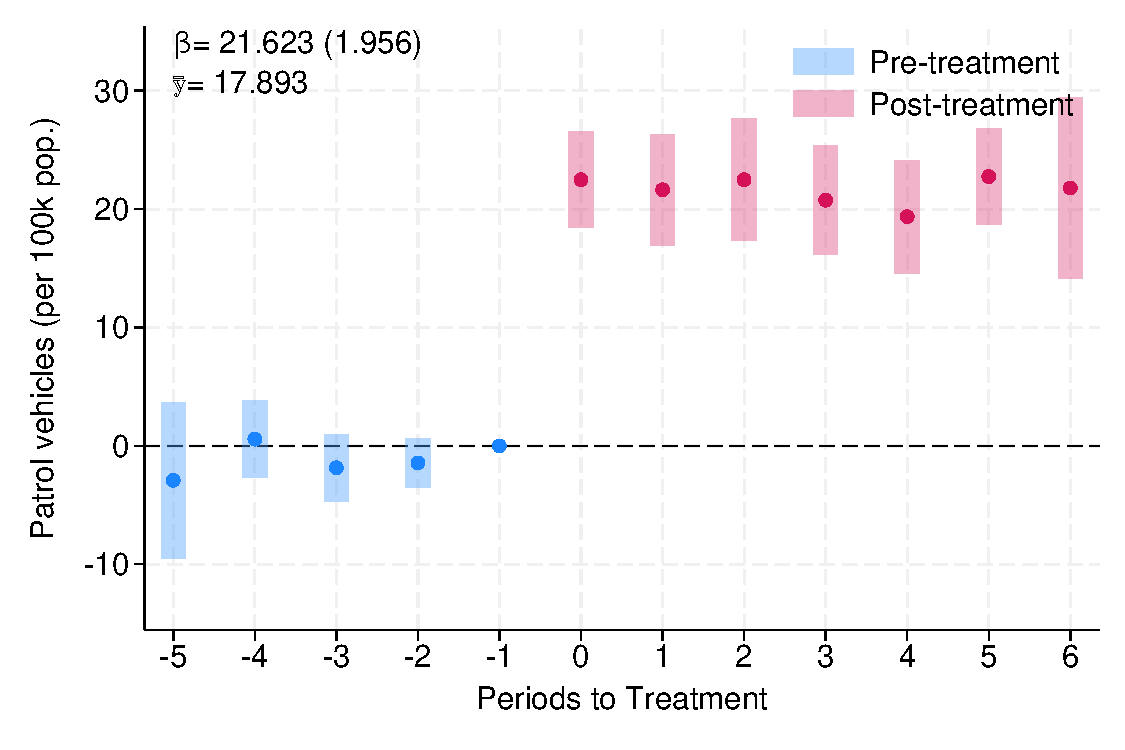
\includegraphics[width=\linewidth]{../manuscript/Graphs/fig4_patrols.pdf}

            \small (b) Effect on the number of patrol vehicles
        \end{minipage}
        \\[4pt]
        \begin{minipage}[t]{0.48\textwidth}
            \centering
            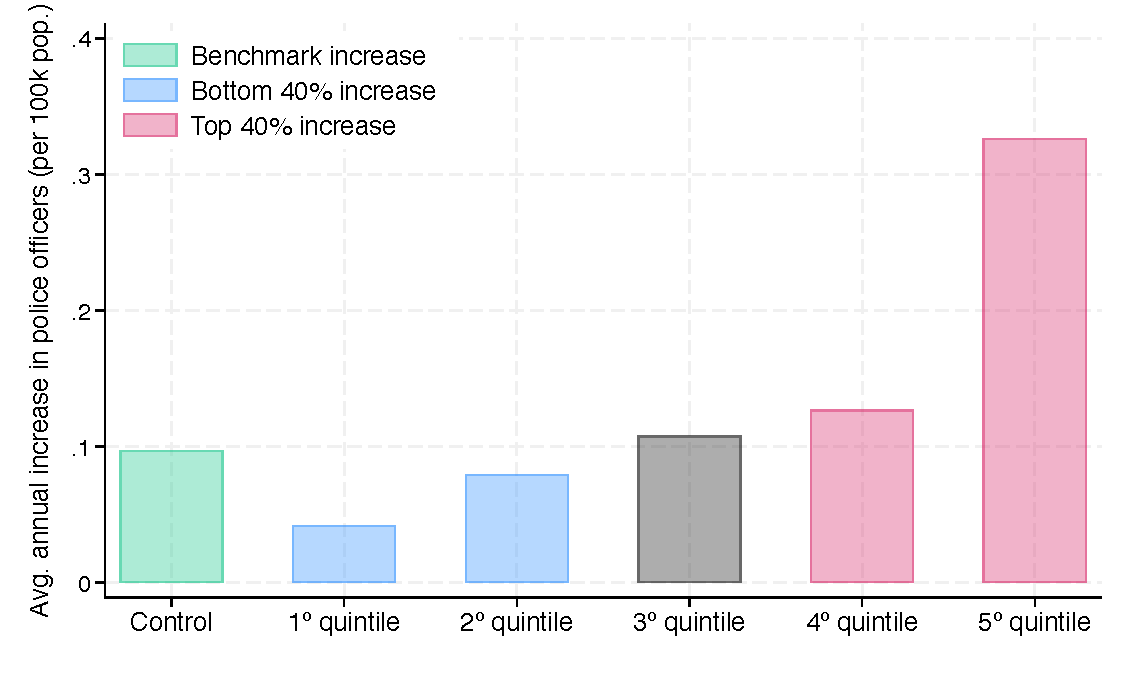
\includegraphics[width=\linewidth]{../manuscript/Graphs/increase_enusc_off_quintiles.pdf}

            \small (c) Distribution of $\Delta$ in police officers
        \end{minipage}
        &
        \begin{minipage}[t]{0.48\textwidth}
            \centering
            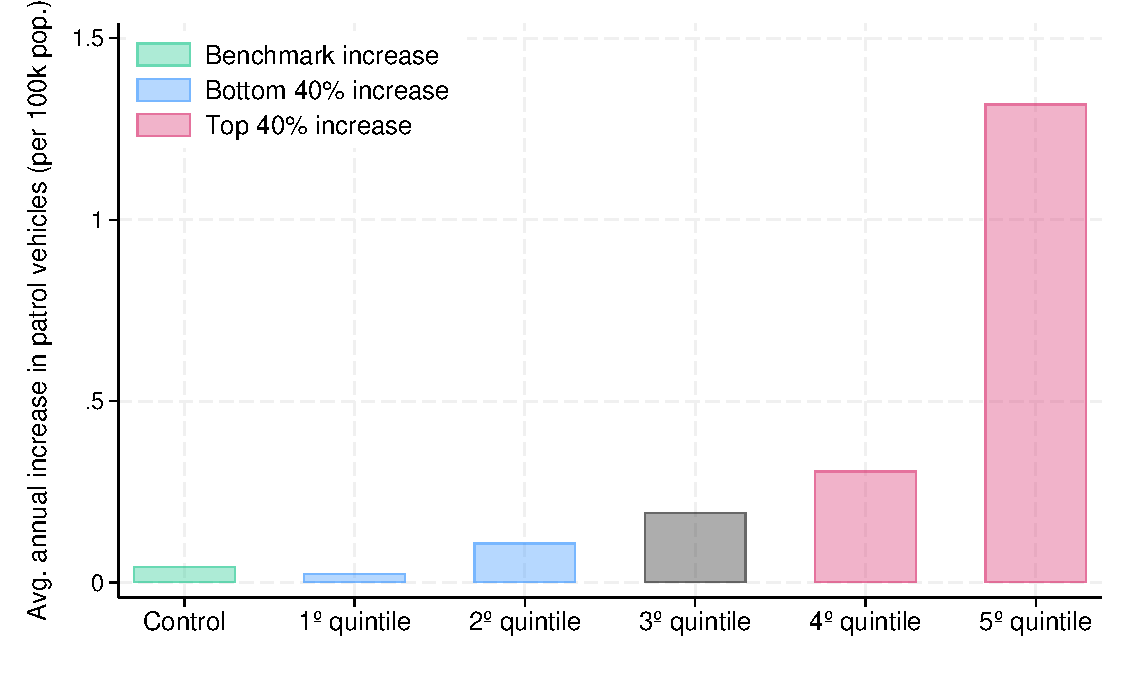
\includegraphics[width=\linewidth]{../manuscript/Graphs/increase_enusc_pv_quintiles.pdf}

            \small (d) Distribution of $\Delta$ in patrol vehicles
        \end{minipage}
        \\[4pt]
        \begin{minipage}[t]{0.48\textwidth}
            \centering
            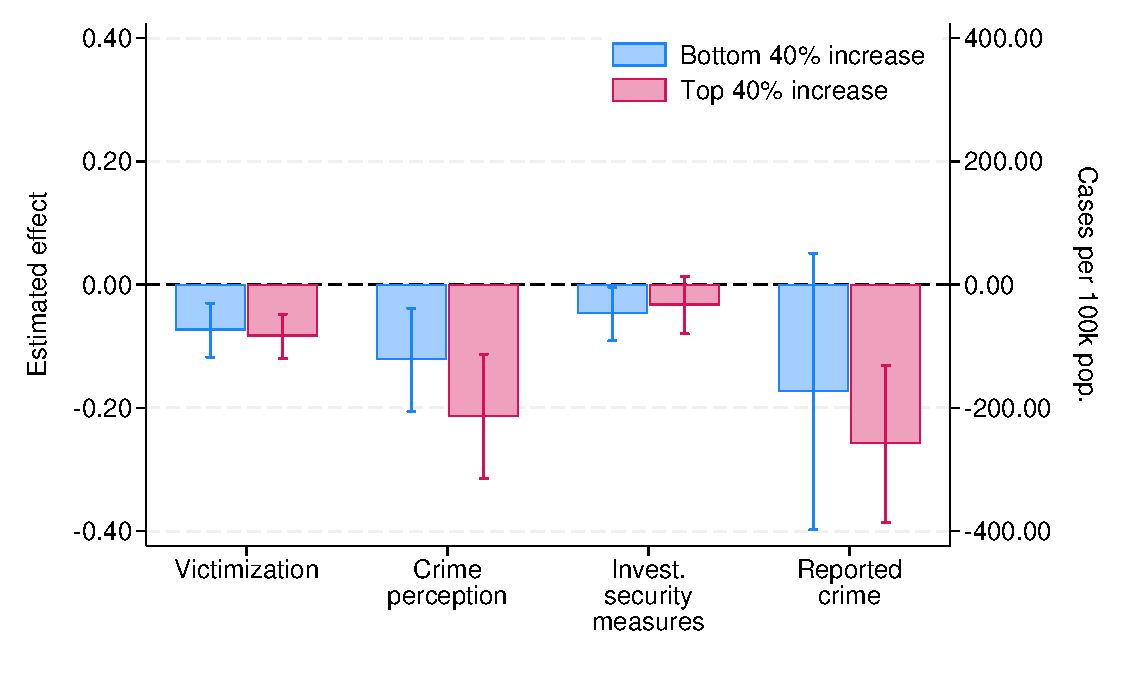
\includegraphics[width=\linewidth]{../manuscript/Graphs/heterogeneity_off.pdf}

            \small (e) Effects by the intensity of $\Delta$ in police officers
        \end{minipage}
        &
        \begin{minipage}[t]{0.48\textwidth}
            \centering
            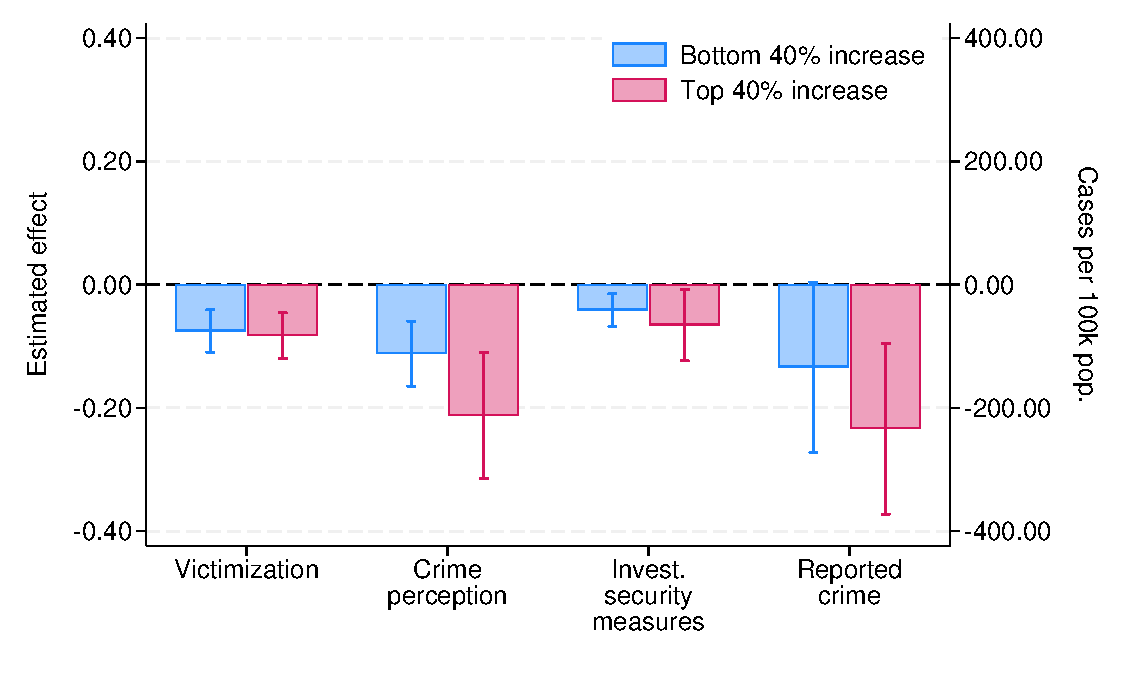
\includegraphics[width=\linewidth]{../manuscript/Graphs/heterogeneity_pv.pdf}

            \small (f) Effects by the intensity of $\Delta$ in patrol vehicles
        \end{minipage}
    \end{tabular}
    \vspace{4pt}
    \begin{minipage}{0.99\textwidth}
    \footnotesize Notes: Panels (a) and (b) show the effect of \emph{Plan Cuadrante} on police officers and patrol vehicles per 100,000 inhabitants. Panels (c) and (d) show the distribution of annual changes in officers and patrol vehicles across municipalities. Panels (e) and (f) report effects by the intensity of resource changes, comparing municipalities in the bottom 40\% and top 40\% of the distribution. The estimation follows \citet{Callaway}. The graphs display estimated coefficients and 95\% confidence intervals. Standard errors are clustered at the municipality level using wild bootstrapping.
    \end{minipage}
\end{figure}
\FloatBarrier
Panels (c) and (d) of Figure \ref{fig:resources} show that the average increase in police resources masks substantial heterogeneity. Municipalities in the bottom 40\% of the resource-change distribution (blue bars) experienced increases close to the average annual variation observed among never treated and not-yet-treated municipalities (green bar). By contrast, municipalities in the top 40\% (red bars) experienced much larger increases, with officers rising by around 22\% and patrol vehicles by around 80\%. If the effects of \emph{Plan Cuadrante} were driven by resource increases alone, we would not expect effects in municipalities whose resource increases were similar to those of the control group. Yet panels (e) and (f) of Figure \ref{fig:resources} show sizeable effects for most crime and crime-perception outcomes even in that low-increase group. While there may be a resource gradient for some crime-perception outcomes, the effects on twelve-month victimization and private investment in security among municipalities with control-like resource increases are close in magnitude to those in municipalities with larger increases. Reassuringly, municipalities in the top and bottom 40\% of the resource-increase distribution do not display differential pre-treatment trends in outcomes or police resources, which suggests that this heterogeneity is not driven by differential pre-existing trends.\footnote{We test for the joint significance of the pre-treatment coefficients between the two groups, separately for the split based on the increase in police officers and the split based on the increase in patrol vehicles. The resulting p-values are, respectively, 0.823 and 0.048 for victimization, 0.059 and 0.379 for crime perception, 0.820 and 0.157 for investment in security measures, and 0.213 and 0.419 for reported crime, as well as 0.616 and 0.444 for police officers and 0.405 and 0.157 for patrol vehicles.}

Although we cannot fully separate the beat policing component from the resource component of the reform---resources may have been important to enable effective implementation of the program, or may explain part of the effects in some municipalities---the fact that municipalities with resource increases similar to those experienced by control municipalities still display sizeable effects indicates that the effects of \emph{Plan Cuadrante} are not driven entirely by resources.\footnote{We also re-estimate the results in Figure \ref{fig:figure02} but controlling for police resources. Online Appendix Table \ref{tab:results_controlbyresources} shows that the magnitude of the estimated effects remains similar for most variables, although the statistical significance is reduced in some estimations. This likely reflects a mechanical feature of the \citet{Callaway} estimation procedure: control variables are not incorporated parametrically, but are instead used to construct the comparison group via outcome regression or propensity-score weighting, so the resulting estimation uncertainty propagates to the ATT standard errors. Note, in addition, that police resources are a bad control---i.e., at least part of their variation is a result of the adoption of \emph{Plan Cuadrante}---so these results should be interpreted cautiously.}\footnote{Table \ref{tab:resourcecorrelates} in Online Appendix \ref{sec:appendixB} examines which factors are associated with a larger increase in police resources upon the adoption of \emph{Plan Cuadrante}.}


\FloatBarrier
%--- Implementation
\begin{figure}[h!]
    \centering
    \caption{Police Resources and Public Safety}
    \label{fig:resources2}
    \begin{subfigure}[t]{0.55\textwidth}
        \centering
        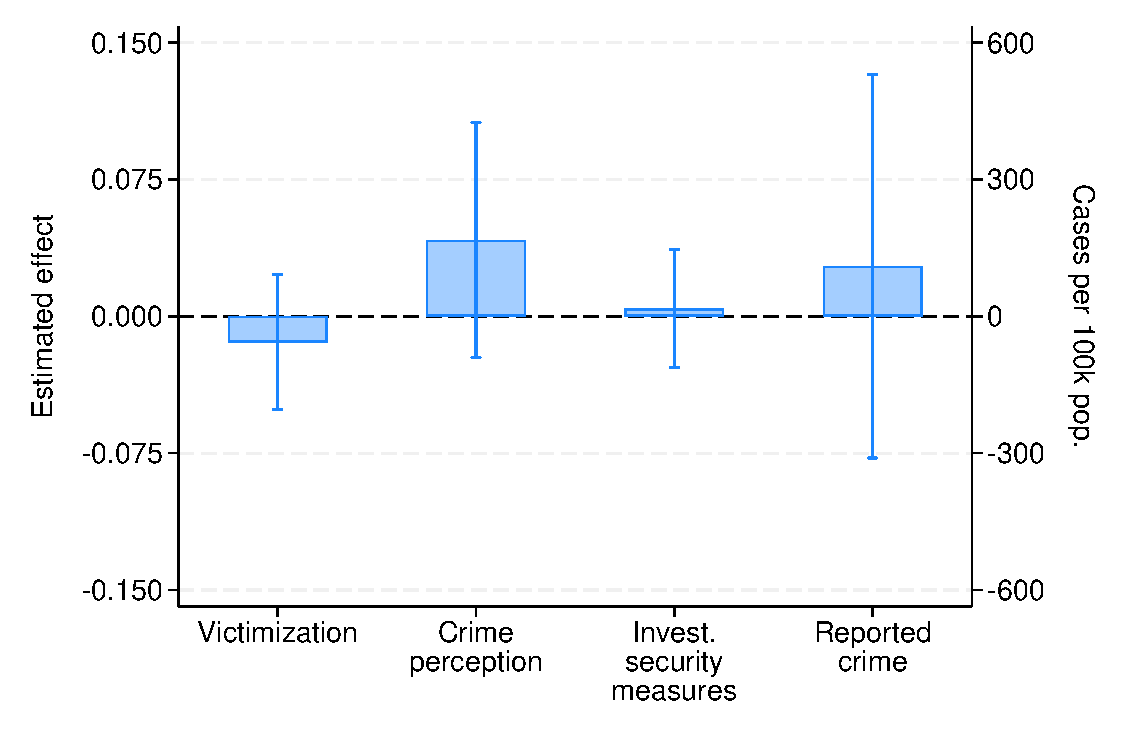
\includegraphics[width=\linewidth]{../manuscript/Graphs/results_SC_att_combined.pdf}
        \caption{Effects of \emph{Seguridad Ciudadana}}
    \end{subfigure}
    \\[6pt]
    \begin{subfigure}[t]{0.55\textwidth}
        \centering
        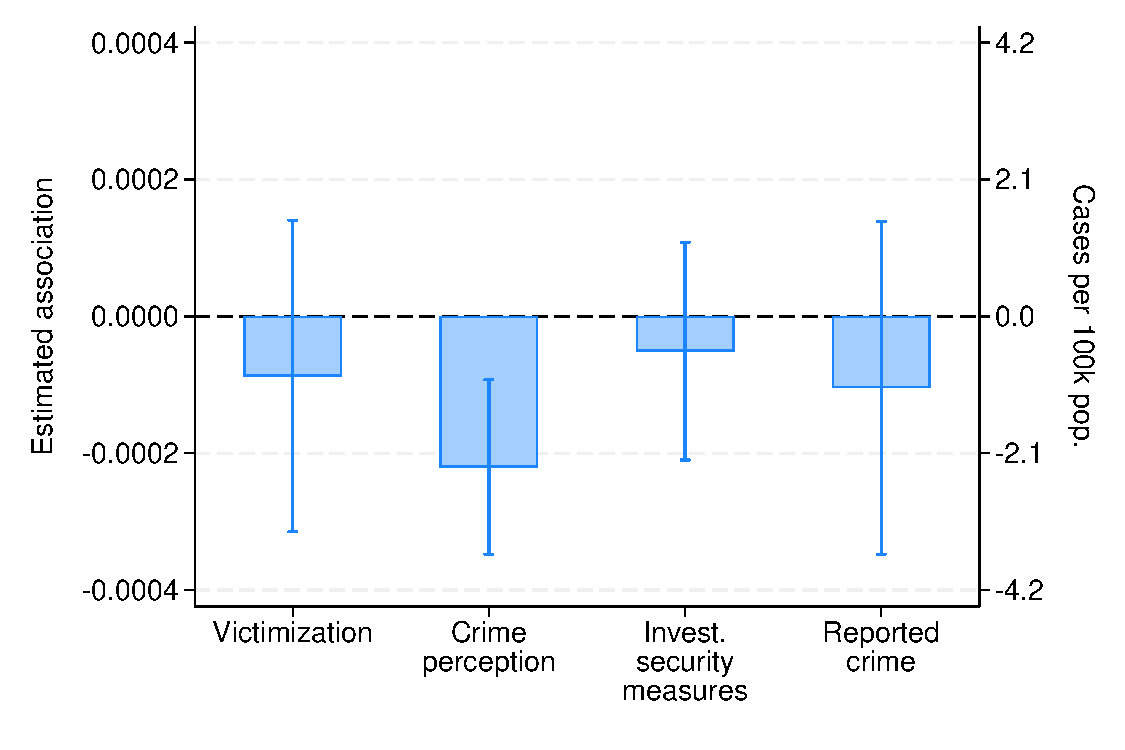
\includegraphics[width=\linewidth]{../manuscript/Graphs/results_corr_novariation_off_santiago.pdf}
        \caption{Association between police officers and effectiveness}
    \end{subfigure}
    \\[6pt]
    \begin{subfigure}[t]{0.55\textwidth}
        \centering
        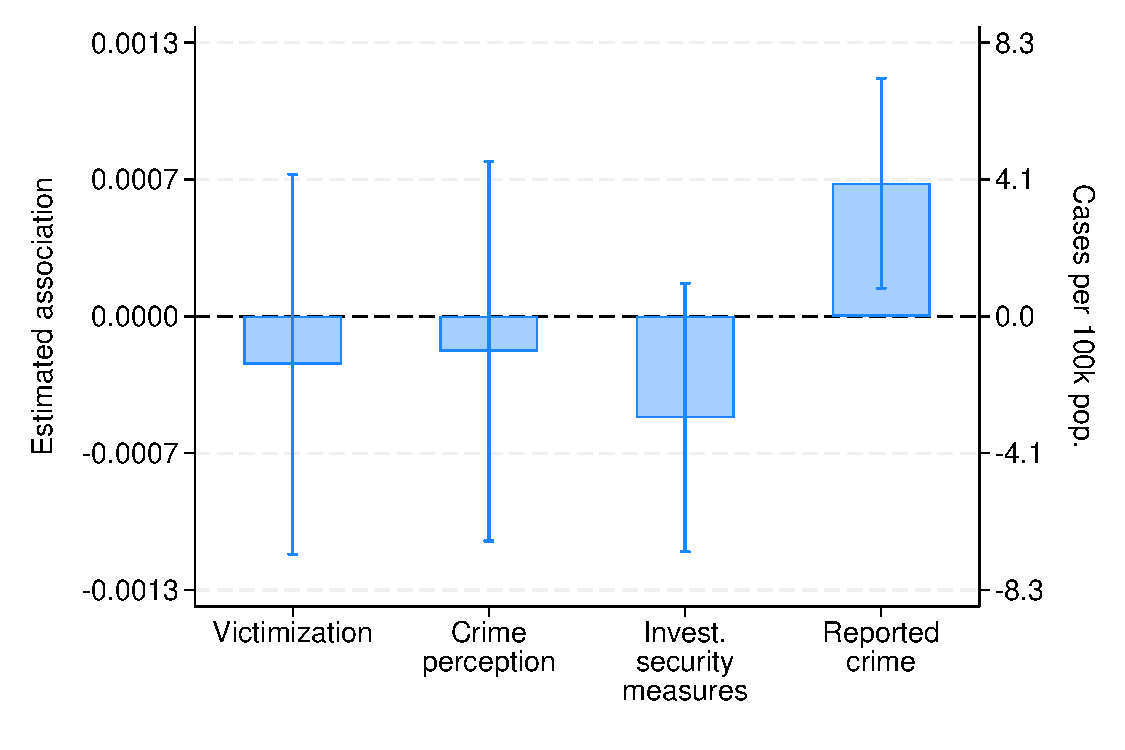
\includegraphics[width=\linewidth]{../manuscript/Graphs/results_corr_novariation_veh_santiago.pdf}
        \caption{Association between patrol vehicles and effectiveness}
    \end{subfigure}
    \\[8pt]
    \begin{minipage}{0.99\textwidth}
    \footnotesize Notes: Panel (a) reports the pooled effect of \emph{Seguridad Ciudadana}, a program that expanded local security personnel to support patrolling and deterrence but did not replicate the deployment-and-strategy features of \emph{Plan Cuadrante}. Panels (b) and (c) report within-municipality associations between police resources and police-effectiveness outcomes among the 41 municipalities of the Santiago Metropolitan Region, all of which had adopted \emph{Plan Cuadrante} by 2000. The regressions include municipality and year fixed effects. Standard errors are clustered at the municipality level using the wild bootstrapping procedure.
    \end{minipage}
\end{figure}
\FloatBarrier

To further investigate whether resource increases alone can explain our results, we assess the effects of \emph{Seguridad Ciudadana}, a program that expanded local security personnel to support patrolling and deterrence, but did not replicate the core deployment-and-strategy features of \emph{Plan Cuadrante}. Using a difference-in-differences specification following \citet{Callaway}, panel (a) of Figure \ref{fig:resources2} shows no significant effects of these resource changes on police effectiveness. Further details about this exercise and the corresponding event-study estimates are reported in Online Appendix \ref{sec:appendixB} and Online Appendix Figure \ref{fig:figureA5}. 


Finally, we study whether variation in police resources in municipalities that had already adopted \emph{Plan Cuadrante} improves public safety and security perceptions. Using ENUSC data and information on resources for 2006--2012 in the 41 municipalities of the Santiago Metropolitan Region---all of which had adopted \emph{Plan Cuadrante} by 2000---we exploit variation in officers and patrol vehicles that is unrelated to program adoption. Panels (b) and (c) of Figure \ref{fig:resources2} show the association between police resources and our main outcomes, conditional on municipality and year fixed effects. With one exception---the association between police officers and crime perception---none of these associations is statistically significant at conventional confidence levels. \footnote{Online Appendix Figure \ref{fig:figureA7B} reports the same exercise and also shows similar results for the broader set of municipalities that adopted \emph{Plan Cuadrante} before 2006 and never-treated municipalities (red bars); see Online Appendix \ref{sec:appendixB} for further details.}

Taken together, these results suggest that resource increases alone do not account for the effects of \emph{Plan Cuadrante}. We next turn to evidence that speaks more directly to the beat-policing components of the reform.

Panel (a) of Figure \ref{fig:police_performance} shows that, following the adoption of \emph{Plan Cuadrante}, households are much more likely to report increased police presence in their neighborhoods. The share of households perceiving increased police presence rises by 35 percentage points (156\%), the share reporting that police pass by their house daily rises by 22 percentage points (59\%), the share reporting never seeing police patrols near their house falls by 10 percentage points (57\%), and complaints about lack of police surveillance fall by around 5 percentage points (20\%). This evidence is consistent with both larger resources and the new deployment model. Yet the latter estimate---the only police-presence outcome for which we can separately estimate effects in municipalities with small and large resource increases---is similar in magnitude across the two groups, which suggests that the increase in police presence is not explained only by larger resource increases (see Online Appendix Figure \ref{fig:heterogeneity_appendix}).\footnote{We cannot estimate heterogeneous effects for other police-presence outcomes, such as the reporting of police passing by or the share of households perceiving an increase in police presence, because those variables are available only in ENUSC rounds 2003, 2005, and 2006, while resource data start in 2006.} More importantly, the broader pattern of results suggests that \emph{Plan Cuadrante} did more than simply increase patrolling intensity. Existing work shows that police presence can reduce crime while officers are present, but that its overall effects may be attenuated when crime is displaced across places or time windows \citep{MASTROBUONI2019, Blanes_Mastrobuoni_2018}. Our results point to something broader. As discussed in Section \ref{results}, we find actual declines in victimization and reported crime, together with no evidence of spillovers to neighboring municipalities. This pattern is more consistent with officers accumulating local knowledge and adapting prevention strategies to local conditions under stable territorial assignment than with a purely mechanical increase in patrol intensity.

Panel (b) of Figure \ref{fig:police_performance} reinforces this interpretation. Households in early-adopting municipalities report better police performance across multiple dimensions. They are 8.1 percentage points (16\%) more likely to rate police performance as good or very good, 7.6 percentage points (11\%) more likely to describe police as efficient, 5 percentage points (6\%) more likely to report that police are helpful, and 4.9 percentage points (7\%) more likely to report that police are well informed. They are also 3.9 percentage points (10\%) less likely to perceive police as corrupt, 7.9 percentage points (21\%) less likely to believe police fail to control crime, and 7.6 percentage points (22\%) less likely to report that police do not perform their duties effectively.\footnote{Information on police performance is only available in ENUSC round 2005. Using this round, we compare perceived police performance in municipalities that adopted \emph{Plan Cuadrante} in 2005 or earlier and in municipalities adopting after 2005. Figure \ref{fig:balance_doseresponse} in Online Appendix \ref{sec:appendixB} shows that the number of years of exposure to \emph{Plan Cuadrante} is positively correlated with perceived police performance. While these exercises on perceived police performance should be interpreted with caution, we show in the same appendix that the timing of future adoption is not correlated with perceived police performance in 2005 for municipalities that had not yet adopted the program by 2005.} %These perceived improvements are consistent with a setting in which officers become better informed about local routines and more effective in how they patrol and respond.

The administrative evidence points in the same direction. Panel (c) of Figure \ref{fig:police_performance} shows that arrests per 100,000 inhabitants increase by 48 (14\%) in our main estimates, even as crime declines overall.\footnote{As with reported crime, this event study is restricted to 5 pre-treatment and 7 post-treatment periods for symmetry with the ENUSC-based analysis; Online Appendix Figure \ref{fig:admin_uncapped} reports the results for arrests using the full set of pre-treatment and post-treatment periods.} This effect is also significant among municipalities with resource increases similar to those in the control group (see Online Appendix Figure \ref{fig:heterogeneity_appendix}). Consistent with this pattern, panel (d) of Figure \ref{fig:police_performance} shows that the arrest rate per reported crime also increases by 1.7 percentage points (10\%), suggesting that a higher share of crimes reported to the police are being solved. Because these gains appear even where resources did not increase more than in control municipalities, they are difficult to reconcile with a pure resource story and are more naturally interpreted as improvements in police effectiveness under the deployment and strategy changes introduced by \emph{Plan Cuadrante}. The corresponding event-study estimates for arrests, the arrest rate per reported crime, and trust in the police in Figure \ref{fig:police_performance} confirm that these changes emerge only after adoption.

Finally, panel (e) of Figure \ref{fig:police_performance} shows a sharp increase in trust in the police in our main specification (Section \ref{results}), consistent with one of the objectives of beat policing, namely bringing officers closer to the community and allowing them to accumulate local knowledge through repeated interaction. Online Appendix Figure \ref{fig:heterogeneity_appendix} shows that this effect remains sizeable both in municipalities that experienced resource increases similar to the control group and in those with larger increases.

Overall, although resources were likely important for implementation and may explain part of the effects in some municipalities, the results in this section indicate that resource changes alone are not enough to explain our findings. The evidence is more consistent with a combination of deployment changes and the strategy adjustments enabled by local knowledge accumulation under permanent assignment to quadrants.

\FloatBarrier
%--- Implementation
\begin{figure}[!ht]
    \centering
    \caption[\emph{Plan Cuadrante} and Changes in Police Performance]{\emph{Plan Cuadrante} and Changes in Police Performance}
    \label{fig:figure05}
    \label{fig:police_performance}
    \label{fig:effectiveness_es}
    \begin{subfigure}[t]{0.44\textwidth}
        \centering
        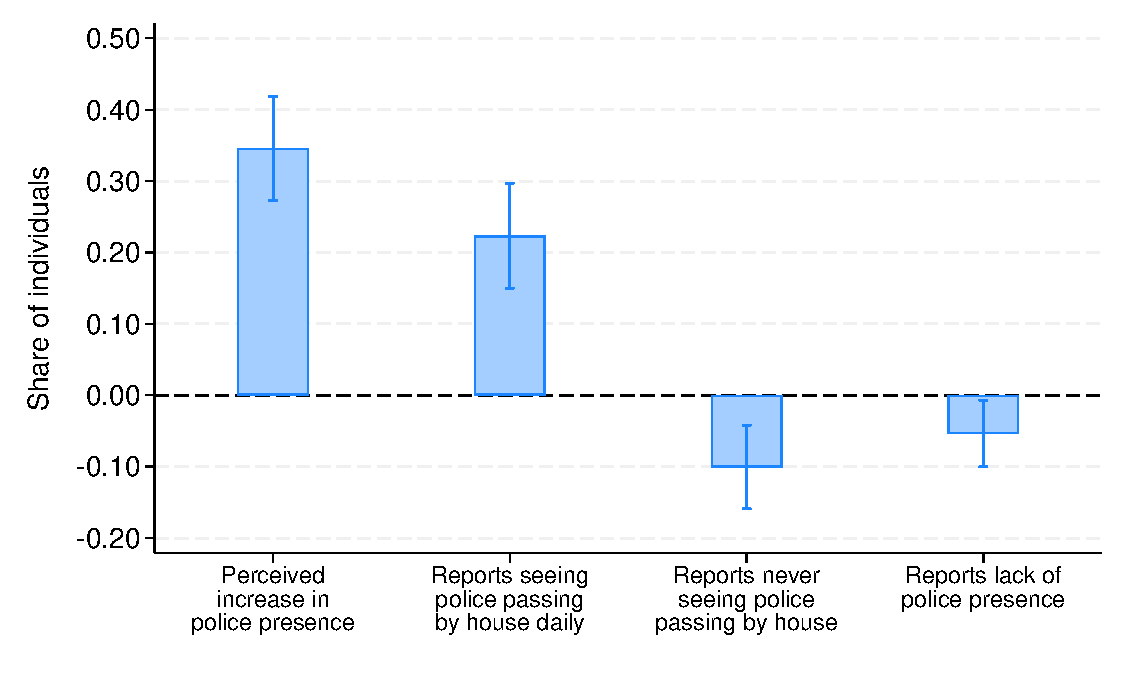
\includegraphics[width=\linewidth]{../manuscript/Graphs/results_policepresence.pdf}
        \caption{Effect on police presence}
    \end{subfigure}\hfill
    \begin{subfigure}[t]{0.44\textwidth}
        \centering
        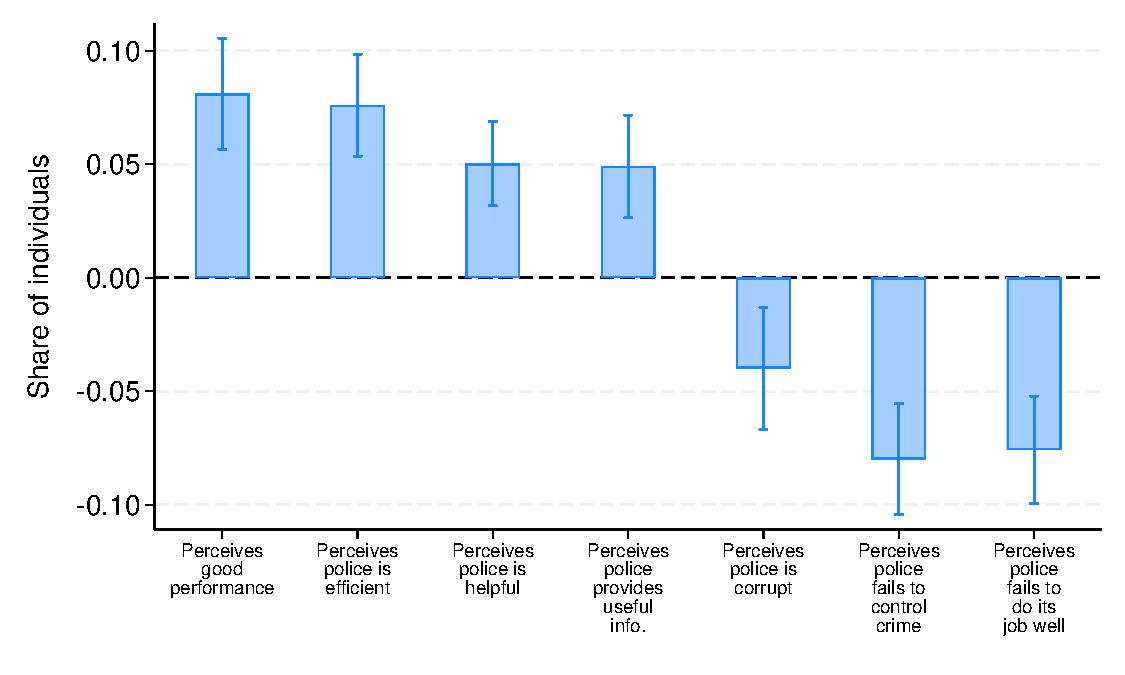
\includegraphics[width=\linewidth]{../manuscript/Graphs/combined_PCttest_2.pdf}
        \caption{Effect on perceived police performance}
    \end{subfigure}
    \\[6pt]
    \begin{subfigure}[t]{0.44\textwidth}
        \centering
        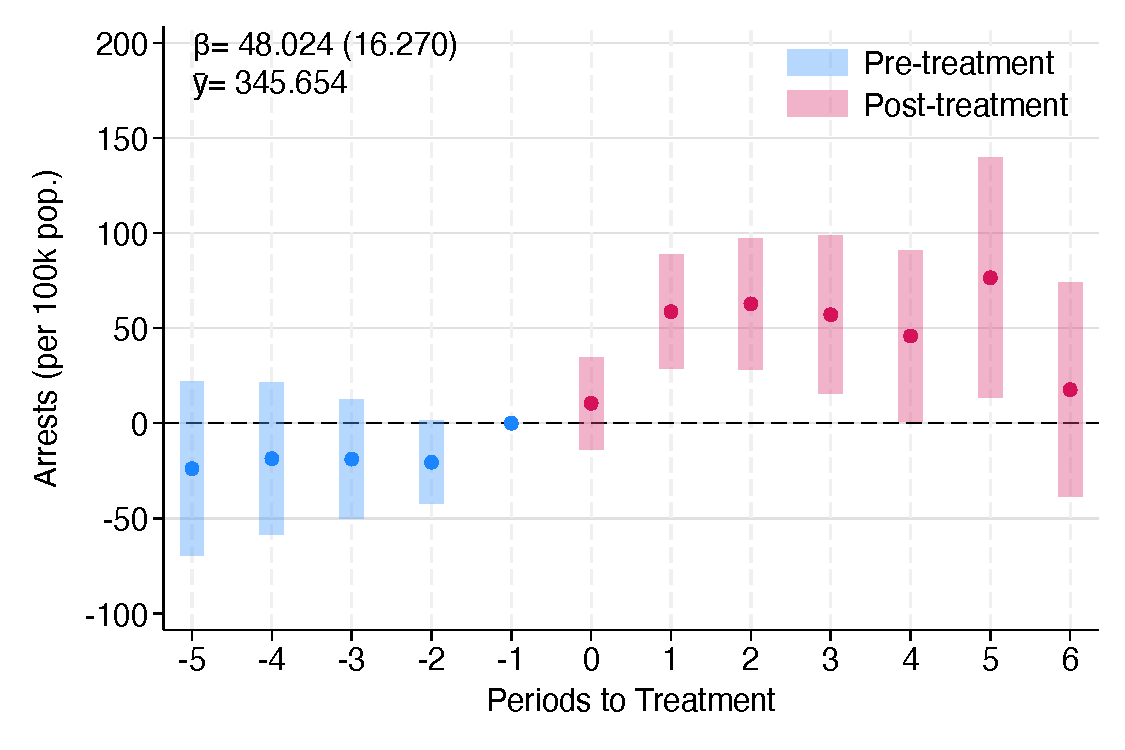
\includegraphics[width=\linewidth]{../manuscript/Graphs/totalarrestscrime_allcomunas.pdf}
        \caption{Arrests (per 100k pop.)}
    \end{subfigure}\hfill
    \begin{subfigure}[t]{0.44\textwidth}
        \centering
        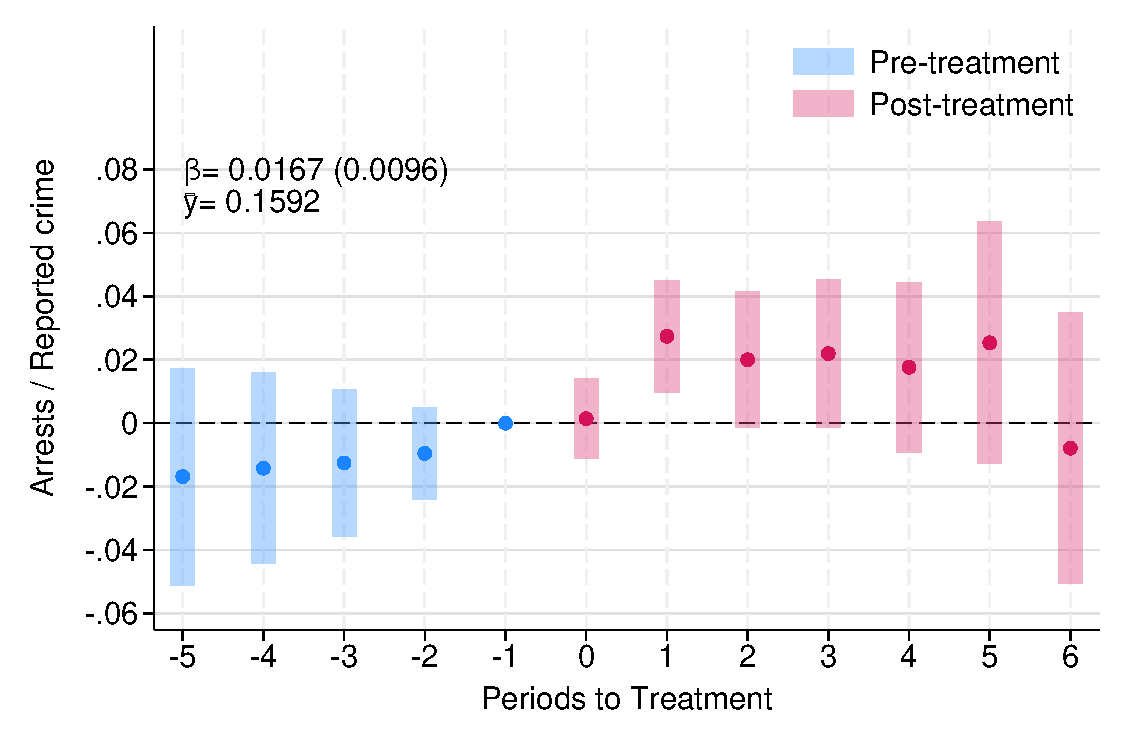
\includegraphics[width=\linewidth]{../manuscript/Graphs/arrests_over_reportedcrime_allcomunas.pdf}
        \caption{Arrests / Reported crime}
    \end{subfigure}
    \\[6pt]
    \begin{subfigure}[t]{0.44\textwidth}
        \centering
        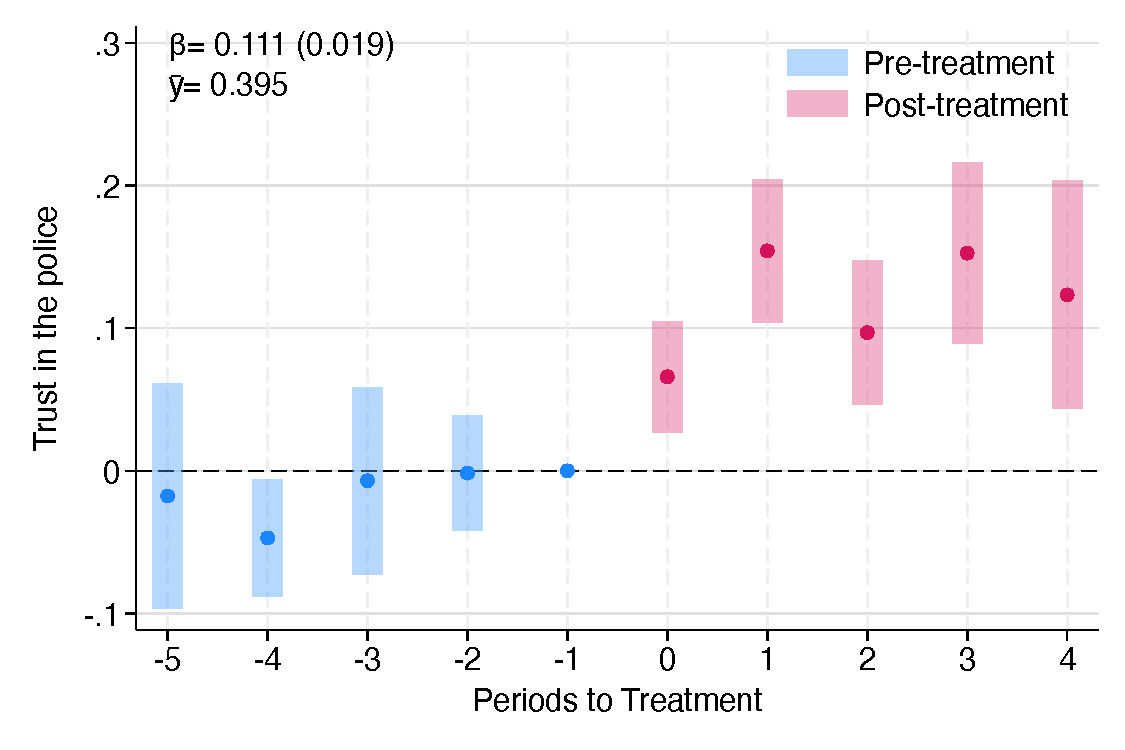
\includegraphics[width=\linewidth]{../manuscript/Graphs/results_trustcarabineros.pdf}
        \caption{Trust in the police}
    \end{subfigure}
    \\[8pt]
    \begin{minipage}{0.99\textwidth}
    \footnotesize Notes: Panel (a) reports the effects on perceived police presence. Panel (b) reports perceived police performance in 2005, comparing municipalities where \emph{Plan Cuadrante} was already implemented before 2006 with municipalities where it was implemented after 2005. Panels (c), (d), and (e) report dynamic event-study estimates for arrests per 100,000 inhabitants, the ratio of arrests to reported crime, and trust in the police. The estimation follows \citet{Callaway}. The graphs display estimated coefficients and 95\% confidence intervals. Standard errors are clustered at the municipality level using the wild bootstrapping procedure.
    \end{minipage}
\end{figure}

\FloatBarrier

%Overall, while resources were arguably important for implementation, the evidence suggests that the beat policing elements---permanent assignment of officers to quadrants and greater local knowledge---were important drivers of the improvements in public safety and security perceptions we document in the paper.



 


% Dani, necesitamos crear dos figuras nuevas combinando parte de los resultados que ya tenemos. 

%% Figure 4: \emph{Plan Cuadrante} and Changes in Police Presence and Resources 
% Panel (a) - Differences in perceptions of police between early and late adopters: 
% Variables to include: 
% Very good/good performance of the police; police is efficient; police is helpful; police provides useful information; police is corrupt; police fails to control crime, police fails to do its job well. Please check well the questions in the survey and define labels with a structure as: "Reports ... " "Perceives ...".
% y-axis: Share of households
% x-axis: Label of the question 

% Panel (b) -  Effect in police presence 
% Bars with diff-in-diff estimates of "Perceived increase in police presence", "Reports seeing police passing by their house daily", "Reports never seeing police passing by their house", "Complaints about lack of police presence"
% y-axis: Share of households 
% x-axis: Periods to treatment

% Panel (c) - Effect in the number of Police Officers
% y-axis: Police officers per 100k inhabitants
% x-axis: Periods to treatment

% Panel (d) - Effect in the number of Police Patrols
% y-axis: Police patrols per 100k inhabitants
% x-axis: Periods to treatment


%% Figure 5: Police Resources and Police Effectiveness

% Panel (a) Distribution of Delta in Police Officers
% Panel (b) Distribution of Delta in Police Patrols 
% Panel (c) Effects by the Intensity of Delta in Police Officers (add bars on "Complaints about lack of police officers")
% Panel (d) Effects by the Intensity of Delta in Police Officers (add bars on "Complaints about lack of police officers")
% Panel (e) Summarize figure A6 in a single panel. One bar per outcome summarizing diff-in-diff estimate. 
% Panel (f) Summarize figure A5 in a single panel. Put ENUSC and admin data together using two y-axis. Combine results for delta officers and delta patrols using different colors for each of them. 



\section{Conclusions}
\label{conclusions}
Beat policing---i.e., assigning the same officers to smaller, well-defined territorial units rather than rotating them over larger ones---has become a widespread strategy to address crime and maintain public safety, yet rigorous causal evidence on its effectiveness remains scarce. Using administrative and survey data from Chile, we show that \emph{Plan Cuadrante}, a reform that introduced beat policing in urban municipalities, substantially reduced victimization and crime perception, while increasing trust in the police. Although its implementation required increasing police resources in some municipalities, we show that resource increases alone cannot account for the observed improvements. The beat policing elements of the reform---permanent assignment to quadrants enabling officers to build local knowledge---seem to be key drivers of its effectiveness.

The reform not only reduced crime incidence but also insecurity perceptions. As a result, households in adopting municipalities reduced their investment in private security measures. Crime rates and perceived victimization risk do not always move together \citep{Ajzenman_Pato}, yet \emph{Plan Cuadrante} reduced both simultaneously. This is an important result as misalignments between actual and perceived risk can lead households to overinvest in private security and distort public expenditure priorities \citep{Minali, Ajzenman_Pato}.

The reform also increased trust in the police---an outcome that has proven particularly difficult to achieve in low- and middle-income countries. Community policing, long regarded as the primary strategy for building police legitimacy, has shown limited effects on both crime and trust in such settings \citep{blair2021, Tobon}. Beat-policing takes a different approach. Rather than relying on community co-production of security, it builds proximity and trust organically through sustained, stable territorial engagement. Our results suggest this organizational logic can be effective even outside developed-country contexts.

Taken together, these results contribute to a broader body of evidence that highlights that the spatial organization of police resources matters. By assigning officers permanently to smaller territorial units, beat policing increases visibility, deepens local knowledge, and improves the capacity of officers to prevent crime and respond to it effectively. This pattern echoes findings from health and education showing that aligning frontline service providers more closely with the communities they serve enhances outcomes \citep{besley2003centralized, Bardhan, Bloom_2015, Basurto}.

While \emph{Plan Cuadrante} was implemented under specific conditions, those conditions help clarify when beat policing is likely to succeed. Two institutional features appear particularly important. First, the absence of significant organized crime during the study period allowed officers to operate repeatedly in their assigned areas without meaningful risk of intimidation or capture, enabling local knowledge and community ties to take root. Second, the relatively high level of professional training in the Chilean police provided a foundation for effectively implementing the reform. Neither of these features is idiosyncratic. They describe an institutional environment that is present, or could be developed, in many settings. Together, they suggest that the gains from beat policing are most likely to materialize when supported by a capable police force operating in a security environment where persistent local engagement is feasible.

\clearpage
\renewcommand\refname{References}
\bibliographystyle{chicago}
\bibliography{Bibliography}

%--- Figures --------------------------------------------------
%--- All figures and tables should be called now from within each section of the manuscript or appendix. Dani, make sure all figures are called in the right place.
%\begin{table}[H]
\centering
\caption{Implementation of \emph{Plan Cuadrante} by Year}
\label{tab:implementation}
\begin{threeparttable}
\begin{tabular}{l c >{\raggedright\arraybackslash}p{10.5cm}}
\toprule
Year & N & Municipalities \\
\midrule
1998--2000 & 44  & Metropolitan Region of Santiago (44 municipalities) \\[3pt]
2002 & 10  & Chiguayante, Concepción, Hualpén, Quilpué, San Antonio, San Pedro de la Paz, Talcahuano, Valparaíso, Villa Alemana, Viña del Mar \\[3pt]
2003 & 2   & Padre Las Casas, Temuco \\[3pt]
2004 & 2   & Antofagasta, Copiapó \\[3pt]
2005 & 7   & Alto Hospicio, Arica, Calama, Curicó, Iquique, Linares, Talca \\[3pt]
2006 & 7   & Coquimbo, La Serena, Los Andes, Ovalle, Rancagua, San Felipe, San Fernando \\[3pt]
2007 & 7   & Chillán, Chillán Viejo, Los Ángeles, Osorno, Puerto Montt, Punta Arenas, Valdivia \\[3pt]
2008 & 9   & Ancud, Castro, Constitución, Coronel, Lota, Peñaflor, Quillota, Rengo, Villarrica \\[3pt]
2009 & 12  & Angol, Aysén, Calera, Concón, Coyhaique, La Unión, Padre Hurtado, Parral, Penco, San Carlos, Tomé, Vallenar \\[3pt]
2011 & 17  & Arauco, Cañete, Cartagena, Cauquenes, Curanilahue, La Ligua, Limache, Molina, Nueva Imperial, Pucón, Puerto Varas, Río Bueno, San Clemente, San Javier, San Vicente, Santa Cruz, Victoria \\[3pt]
2012 & 20  & Cabrero, Calbuco, Casablanca, Chimbarongo, Collipulli, Curacaví, El Monte, Graneros, Illapel, Isla de Maipo, Lautaro, Machalí, Mostazal, Mulchén, Nacimiento, Natales, Panguipulli, Quellón, Quintero, Tocopilla \\[3pt]
2013 & 13  & Bulnes, Laja, Las Cabras, Lebu, Llaillay, Loncoche, Longaví, Los Álamos, Maule, Requínoa, Teno, Vicuña, Yumbel \\
\midrule
Total & 150 & \\
\bottomrule
\end{tabular}
\begin{tablenotes}[flushleft]
\footnotesize
\item Note: \textit{N} is the number of municipalities that adopted \emph{Plan Cuadrante} in each year. Data shared by Carabineros de Chile.
\end{tablenotes}
\end{threeparttable}
\end{table}


%--- ONLINE APPENDIX --------------------------------------------------
\FloatBarrier
\clearpage

\thispagestyle{empty}\setcounter{page}{0}
\vspace*{.2in}

\begin{center}
\textbf{\Large Boots in the Beat: Effects of Beat Policing on Victimization and Crime Perception}$^\dagger$
\end{center}
\vspace{.25in}

\begin{center}\large
  Andr\'es Barrios-Fern\'andez \hspace{.12in}
  Jorge Garc\'ia-Hombrados \hspace{.12in}
  Daniel P\'erez-Parra
\end{center}

\medskip

\begin{center}\large
\today \\
\href{https://andresbarriosf.github.io/police_reform.pdf}{Latest Version}
\end{center}

\mythanks{\hspace{-.25in}$^\dagger$
Corresponding author: Andrés Barrios-Fernández (andres.bafer@alumni.lse.ac.uk). School of Business and Economics. Universidad de los Andes, Chile. Monseñor Álvaro del Portillo 12.455. Las Condes. Santiago. We thank Carabineros de Chile for granting us access to the administrative data we use in this project. Andr\'es Barrios-Fernández acknowledges the financial support of Fondecyt Regular Project 1261817.}

\onehalfspacing
\appendix

\addtocontents{toc}{\protect\setcounter{tocdepth}{\arabic{tocdepth}}}
\tableofcontents
\newpage

%---- Online Appendix A - Implementation Details
\clearpage
\section{The Rollout of \emph{Plan Cuadrante}} \label{sec:appendixA}

\setcounter{figure}{0}
\renewcommand{\thefigure}{\Alph{section}\arabic{figure}}
\setcounter{table}{0}
\renewcommand{\thetable}{\Alph{section}\arabic{table}}

This Online Appendix provides additional information on the staggered rollout of the \emph{Plan Cuadrante} program.


\emph{Plan Cuadrante} was launched in 1998, initially as a pilot program in a few municipalities in the southern part of the city of Santiago. This initial phase aimed to test the plan's implementability. The six-month pilot revealed promising outcomes, which led to its broader implementation despite the need for additional resources and personnel.

By 2000, the \emph{Plan Cuadrante} had expanded to 44 municipalities in Santiago, covering approximately 96.1\% of the city’s population. This expansion was based on expert recommendations and the division of urban areas into manageable patrol zones. The plan was then implemented gradually throughout urban municipalities in Chile. The staggered expansion of the \emph{Plan Cuadrante} beyond Santiago was, in principle, meant to follow a prioritization based on a weighted index of victimization, police resource deficits, drug prevalence, unemployment, and demand for police services, with annual entry determined by available budget. The weights assigned to each component changed on a yearly basis and, in practice, Budget Office evaluations show that adoption diverged from this ranking for undocumented reasons, so the rule operated more as a loose guideline than as a binding assignment mechanism \citep{DIPRES2014}.\footnote{We requested information from Carabineros about the index, its inputs and weights but we were not granted systematic access to this information.}


The plan saw significant growth between 2002 and 2006. In 2002, it extended beyond Santiago into the V and VIII Regions, adding ten new municipalities. The expansion continued from 2003 to 2006, with 18 additional municipalities incorporated into the plan. By 2006, the \emph{Plan Cuadrante} covered a total of 72 municipalities across Chile. Between 2007 and 2009, the plan expanded to include 28 more municipalities, reaching the 100 municipalities covered by the \emph{Plan Cuadrante}. The \emph{Plan Cuadrante} faced significant challenges in 2010 due to the earthquake that struck Chile. The disaster necessitated a reallocation of resources to support recovery efforts, temporarily halting the plan’s expansion. Despite this setback, the \emph{Plan Cuadrante} resumed its implementation in 2011. Between 2011 and 2013, the plan was expanded to include an additional 50 municipalities, bringing the total to 150 across Chile. Tables \ref{tab:sum_statsA2} and \ref{tab:sum_statsA3} present summary statistics at the household and at the municipality level of the municipalities implementing \emph{Plan Cuadrante} in the period that we study. 

\vspace{5mm}
\begin{table}[H]
\centering
\caption{Implementation of \emph{Plan Cuadrante} by Year}
\label{tab:implementation}
\begin{threeparttable}
\begin{tabular}{l c >{\raggedright\arraybackslash}p{10.5cm}}
\toprule
Year & N & Municipalities \\
\midrule
1998--2000 & 44  & Metropolitan Region of Santiago (44 municipalities) \\[3pt]
2002 & 10  & Chiguayante, Concepción, Hualpén, Quilpué, San Antonio, San Pedro de la Paz, Talcahuano, Valparaíso, Villa Alemana, Viña del Mar \\[3pt]
2003 & 2   & Padre Las Casas, Temuco \\[3pt]
2004 & 2   & Antofagasta, Copiapó \\[3pt]
2005 & 7   & Alto Hospicio, Arica, Calama, Curicó, Iquique, Linares, Talca \\[3pt]
2006 & 7   & Coquimbo, La Serena, Los Andes, Ovalle, Rancagua, San Felipe, San Fernando \\[3pt]
2007 & 7   & Chillán, Chillán Viejo, Los Ángeles, Osorno, Puerto Montt, Punta Arenas, Valdivia \\[3pt]
2008 & 9   & Ancud, Castro, Constitución, Coronel, Lota, Peñaflor, Quillota, Rengo, Villarrica \\[3pt]
2009 & 12  & Angol, Aysén, Calera, Concón, Coyhaique, La Unión, Padre Hurtado, Parral, Penco, San Carlos, Tomé, Vallenar \\[3pt]
2011 & 17  & Arauco, Cañete, Cartagena, Cauquenes, Curanilahue, La Ligua, Limache, Molina, Nueva Imperial, Pucón, Puerto Varas, Río Bueno, San Clemente, San Javier, San Vicente, Santa Cruz, Victoria \\[3pt]
2012 & 20  & Cabrero, Calbuco, Casablanca, Chimbarongo, Collipulli, Curacaví, El Monte, Graneros, Illapel, Isla de Maipo, Lautaro, Machalí, Mostazal, Mulchén, Nacimiento, Natales, Panguipulli, Quellón, Quintero, Tocopilla \\[3pt]
2013 & 13  & Bulnes, Laja, Las Cabras, Lebu, Llaillay, Loncoche, Longaví, Los Álamos, Maule, Requínoa, Teno, Vicuña, Yumbel \\
\midrule
Total & 150 & \\
\bottomrule
\end{tabular}
\begin{tablenotes}[flushleft]
\footnotesize
\item Note: \textit{N} is the number of municipalities that adopted \emph{Plan Cuadrante} in each year. Data shared by Carabineros de Chile.
\end{tablenotes}
\end{threeparttable}
\end{table}


\begin{table}[H]
\centering
\caption{Summary Statistics -- ENUSC sample}
\label{tab:sum_statsA2}
\begin{threeparttable}
\begin{tabular}{l r r r r r}
\toprule
 & Mean & SD & Min & Max & N \\
\midrule
\multicolumn{6}{@{}l}{\textit{Household}} \\
\quad Socioeconomic status               & 3.58  & 0.73  & 1    & 5    & 99,298 \\
\quad Victimization                    & 0.26  & 0.44  & 0    & 1    & 99,298 \\
\quad Crime perception (neighborhood)  & 0.38  & 0.49  & 0    & 1    & 95,598 \\
\quad Crime perception (municipality)  & 0.66  & 0.48  & 0    & 1    & 96,794 \\
\quad Crime perception (country)       & 0.79  & 0.41  & 0    & 1    & 98,525 \\
\quad Trust in the police              & 0.44  & 0.50  & 0    & 1    & 51,445 \\
\quad Investment in security measures  & 0.21  & 0.40  & 0    & 1    & 99,298 \\
\quad \emph{Plan Cuadrante} (year)                  & 2007  & 1.85  & 2005 & 2012 & 97,847 \\
\addlinespace
\multicolumn{6}{@{}l}{\textit{Household member interviewed}} \\
\quad Female                      & 0.55  & 0.50  & 0  & 1  & 99,298 \\
\quad Age                         & 43.87 & 17.95 & 15 & 99 & 99,298 \\
\quad Primary school attendance   & 0.98  & 0.14  & 0  & 1  & 99,298 \\
\quad Secondary school attendance & 0.72  & 0.45  & 0  & 1  & 99,298 \\
\quad University attendance       & 0.20  & 0.40  & 0  & 1  & 99,298 \\
\bottomrule
\end{tabular}
\begin{tablenotes}[flushleft]
\footnotesize
\item Note: This table presents summary statistics from the ENUSC sample, covering the 47 municipalities used in the survey-based analysis (46 that adopted \emph{Plan Cuadrante} between 2005 and 2012 plus one never-treated municipality). Socioeconomic status is a 1 to 5 measure produced by ENUSC surveys and based on self-reported socioeconomic strata, being 1 the highest ranked and 5 the lowest. Crime perception is equal to 1 if the interviewed person reports that crime has increased in the last 12 months. The \emph{Plan Cuadrante} (year) row is computed over treated municipalities only.
\end{tablenotes}
\end{threeparttable}
\end{table}

\begin{table}[H]
\centering
\caption{Summary Statistics -- Administrative municipality level sample}
\label{tab:sum_statsA3}
\begin{threeparttable}
\begin{tabular}{l r r r r r}
\toprule
 & Mean & SD & Min & Max & N \\
\midrule
\multicolumn{6}{@{}l}{\textit{Panel A. Reported-crime sample (292 municipalities)}} \\
\quad Reported crime (per 100k pop.)            & 1,732.39 & 1,036.68 & 0.00   & 11,434.40 & 4,371 \\
\quad Arrests (per 100k pop.)                   & 332.07   & 271.75   & 0.00   & 1,712.30  & 3,504 \\
\quad Poverty rate (\%)                         & 25.74    & 9.72     & 5.65   & 58.33     & 3,720 \\
\quad Pop.\ density (pop./km\textsuperscript{2}) & 63.51   & 140.47   & 0.09   & 1,109.58  & 4,065 \\
\quad \emph{Plan Cuadrante} (year)                     & 2010     & 2.82     & 2003   & 2013      & 1,440 \\
\addlinespace
\multicolumn{6}{@{}l}{\textit{Panel B. Arrests sample (281 municipalities)}} \\
\quad Reported crime (per 100k pop.)            & 1,684.74 & 1,014.67 & 0.00   & 11,434.40 & 4,209 \\
\quad Arrests (per 100k pop.)                   & 313.21   & 251.23   & 0.00   & 1,712.30  & 3,372 \\
\quad Poverty rate (\%)                         & 26.01    & 9.72     & 5.65   & 58.33     & 3,570 \\
\quad Pop.\ density (pop./km\textsuperscript{2}) & 57.90   & 127.30   & 0.09   & 1,109.58  & 3,900 \\
\quad \emph{Plan Cuadrante} (year)                     & 2010     & 2.26     & 2006   & 2013      & 1,275 \\
\bottomrule
\end{tabular}
\begin{tablenotes}[flushleft]
\footnotesize
\item Note: The table reports municipality-level summary statistics for the two administrative estimation samples used in the paper. Panel A covers the 292 municipalities in the reported-crime sample (municipalities adopting \emph{Plan Cuadrante} from 2003 onward plus never-treated); Panel B the 281 municipalities in the arrests sample (adopters from 2006 onward plus never-treated --- municipalities adopting in 2005 are excluded because arrest data begin that year, leaving no pre-treatment period). Reported crime and arrests are measured per 100,000 inhabitants over 2002--2016 and 2005--2016, respectively. Minimum reported crime and arrests of zero correspond to tiny, remote never-treated comunas (e.g., Juan Fernández, Cabo de Hornos). The \emph{Plan Cuadrante} (year) row is computed over treated municipalities only. Data from the Undersecretary for Crime Prevention.
\end{tablenotes}
\end{threeparttable}
\end{table}

\clearpage


%---- Online Appendix B - Additional Results
\clearpage
\section{Additional Results} \label{sec:appendixB}

\setcounter{figure}{0}
\renewcommand{\thefigure}{\Alph{section}\arabic{figure}}
\setcounter{table}{0}
\renewcommand{\thetable}{\Alph{section}\arabic{table}}

This Online Appendix expands on some of the analyses presented in the main body of the paper. First, it characterizes the treated municipalities in our analytical samples relative to the average Chilean municipality. Second, it shows the effects of \emph{Plan Cuadrante} on different types of crime. Third, it documents some differences in results associated to private investment in security depending on household SES. Fourth, it presents two new analyses that suggest that changes in police resources associated to the adoption of the \emph{Plan Cuadrante} are not enough to explain its results. Fifth, it examines what factors are associated with a larger increase in police resources across municipalities adopting \emph{Plan Cuadrante}. Sixth, it presents the results of a new exercise that shows that increases in police resources unrelated to \emph{Plan Cuadrante} do not generate major gains in police effectiveness. Finally, it shows that the comparison of perceived police performance between early and late adopters is not confounded by differences in adoption timing.


\subsection{Characterization of the Analytical Samples}
\label{sec:ext_validity}

The treated municipalities in our analytical samples are geographically distributed across the country. As shown in Figure \ref{fig:pcsp_maps}, the 46 treated municipalities in the ENUSC-based sample span Chile from north to south, covering a wide range of geographic and socioeconomic contexts, and together account for approximately 27\% of Chile's population. The 96 treated municipalities in the administrative data sample provide even broader national coverage, together accounting for over half of Chile's population.

Table \ref{tab:comparing_samples} characterizes the treated municipalities in each analytical sample relative to all Chilean municipalities (Column 1), all \emph{Plan Cuadrante} municipalities (Column 2), the always-treated municipalities excluded from our estimation samples (Column 3), and never-treated municipalities (Column 6). Columns (4) and (5) report characteristics for the treated municipalities in the ENUSC and administrative data analytical samples respectively. On several dimensions our samples broadly resemble the overall Chilean population: the poverty rate of the 46 treated municipalities in the ENUSC sample (21.7\%) and the 96 treated municipalities in the administrative data sample (24.0\%) are both close to the national average of 23.7\%, and the crime rates of the treated ENUSC municipalities closely track the average across all \emph{Plan Cuadrante} municipalities (2,202 vs.\ 2,132 per 100,000 inhabitants). They do differ on other dimensions---particularly crime rates relative to all Chilean municipalities and population density---but both differences have natural explanations. Higher crime rates are expected because \emph{Plan Cuadrante} exclusively targeted urban municipalities, where crime is more prevalent. The lower-than-average population density in our samples (215 and 135 inhabitants per km$^2$, vs.\ a national mean of 870) reflects the fact that the most densely populated \emph{Plan Cuadrante} municipalities---those of the Santiago metropolitan area---were the earliest adopters of the program and are therefore excluded from our analytical samples as always-treated. 

\begin{figure}[h!]
    \centering
    \caption{Geographic Distribution of \emph{Plan Cuadrante}}
    \label{fig:pcsp_maps}
    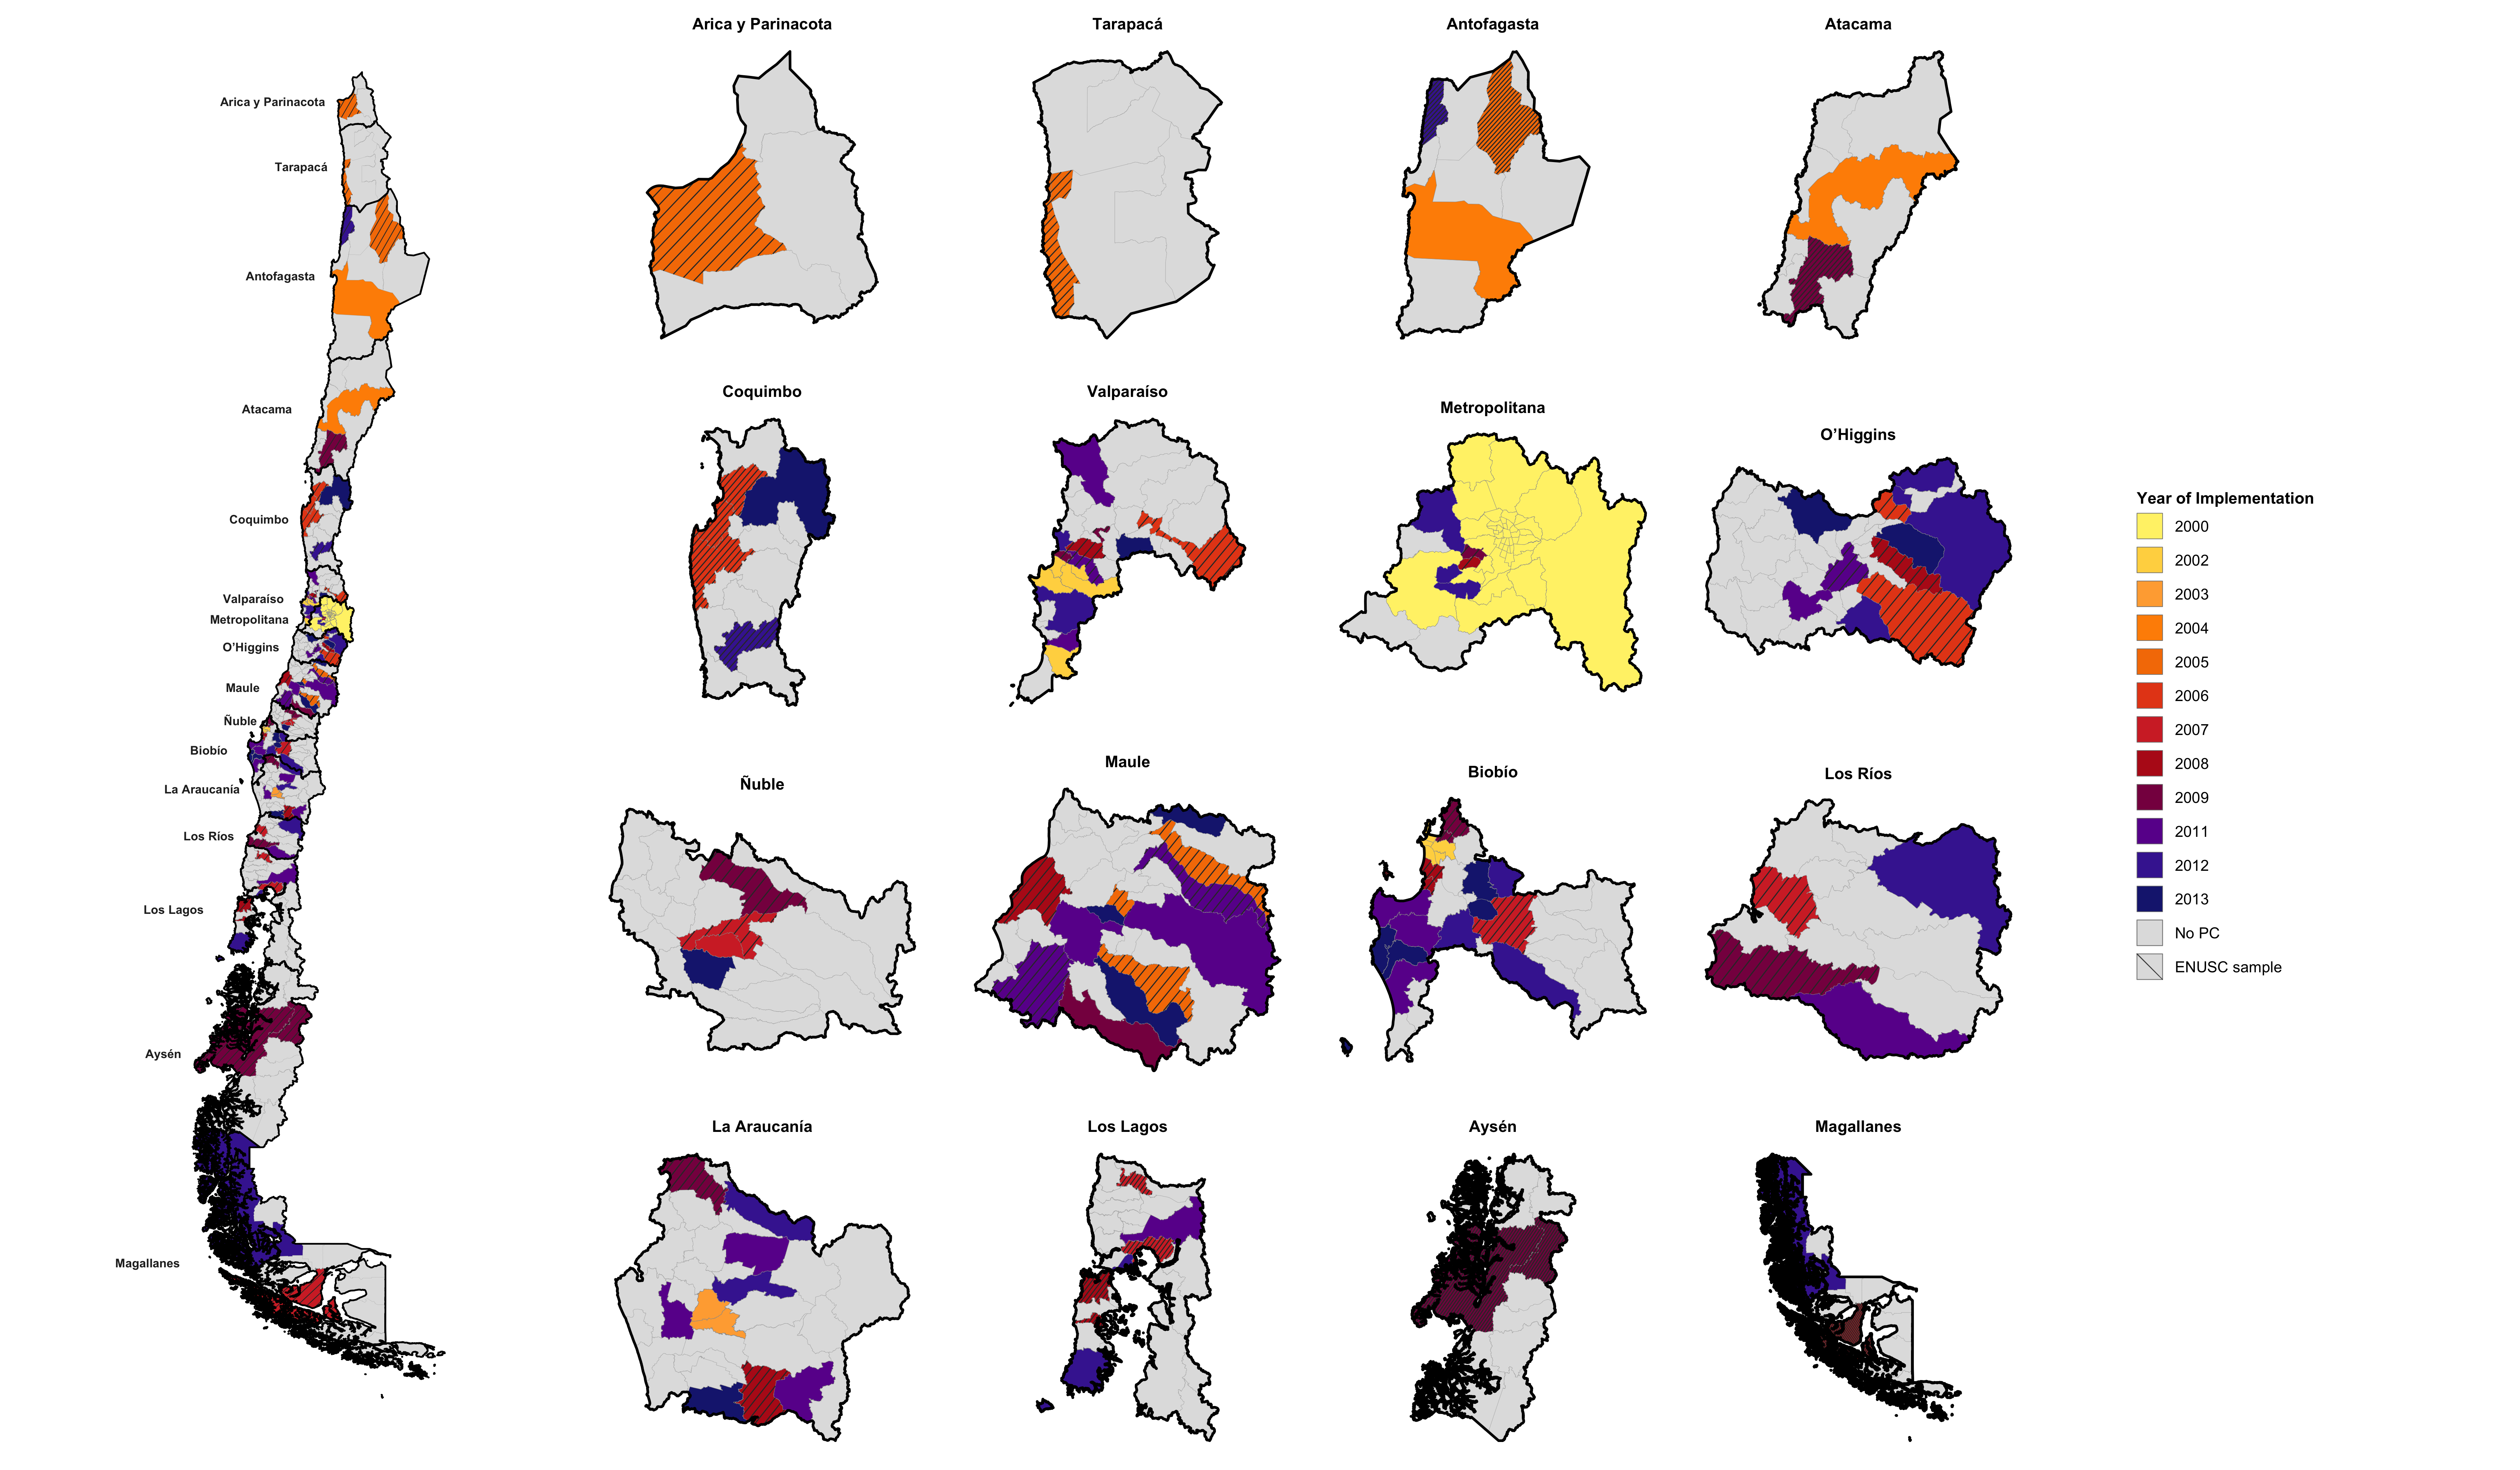
\includegraphics[width=\textwidth]{../manuscript/Graphs/mapa_PCSP_Chile_combinado.png}
    \begin{minipage}{0.95\textwidth}
    \footnotesize
    Notes: This figure shows the spatial rollout of \emph{Plan Cuadrante} across Chilean municipalities. The national map (left) is displayed alongside the 16 regional maps (right) for closer inspection. The color of each treated municipality indicates its year of program adoption, ranging from 2000 (lightest) to 2013 (darkest), following the legend. Municipalities shown in light grey were never treated under PC. Diagonal hatching identifies the 46 treated municipalities in the analytical sample used to estimate the effects on ENUSC outcomes.
    \end{minipage}
\end{figure}


\begin{table}[H]
\caption{Baseline characteristics by subsample}
\label{tab:comparing_samples}
\begin{center}
\resizebox{\textwidth}{!}{
\begin{threeparttable}
\begin{tabular}{l cccccc}
\toprule
&  & \multicolumn{4}{c}{PC municipalities}  & \\
\cmidrule(lr){3-6}
& (1) & (2) & (3) & (4) & (5) & (6) \\
& All & All PC & Always- & Treated & Treated & Never- \\
& municipalities & municipalities & treated & ENUSC & admin.\ data & treated \\
\midrule
Reported crime (per 100k pop.) &     1,650.23 &     2,132.29 &     2,437.25 &     2,202.06 &     1,976.59 &     1,282.47 \\
Arrests (per 100k pop.)        &       267.62     &       442.08     &       606.01     &       459.05     &       358.11     &       134.11     \\
Poverty rate (\%)              &        23.73     &        20.50     &        14.88     &        21.73     &        23.96     &        26.82     \\
Pop.\ density (pop./km$^2$)   &       870.28 &     1,904.14 &     4,593.32 &       215.52 &       134.50 &        27.02 \\
Population                     &    57,857.22         &   117,975.43         &   187,558.74         &   113,079.74         &    81,532.84         &    11,612.44         \\
\midrule
Municipalities                 &          346            &          150            &           58            &           46            &           96            &          196            \\
\bottomrule
\end{tabular}
\begin{tablenotes}[flushleft]
\footnotesize{\item Note: Reported crime, poverty rate, population density, and population are measured as of 2003; arrests are measured as of 2005, the first year for which arrest data are available. Column (1) includes all municipalities in Chile. Column (2) includes all PC municipalities. Column (3) restricts to municipalities that adopted \emph{Plan Cuadrante} before 2005, the always-treated in our sample, which are therefore excluded from our estimation samples (as depicted in Figure 1, panel (a)). Column (4) restricts to treated municipalities in the analytical sample using the ENUSC data. Column (5) restricts to treated municipalities included in the analytical sample using the administrative data. Column (6) includes never-treated municipalities.}
\end{tablenotes}
\end{threeparttable}}
\end{center}
\end{table}


\clearpage

\subsection{Effects of \emph{Plan Cuadrante} on Different Types of Crime}
Figure \ref{fig:figureA8} displays the effects of \emph{Plan Cuadrante} on victimization by type of crime, showing beneficial effects for both violent and property crimes. 


\begin{figure}[h!]
    \centering
    \caption{The Effects of \emph{Plan Cuadrante} on Victimization and Reported Crime by Type of Crime}
    \label{fig:figureA8}
    \begin{subfigure}{0.45\textwidth}
        \centering
        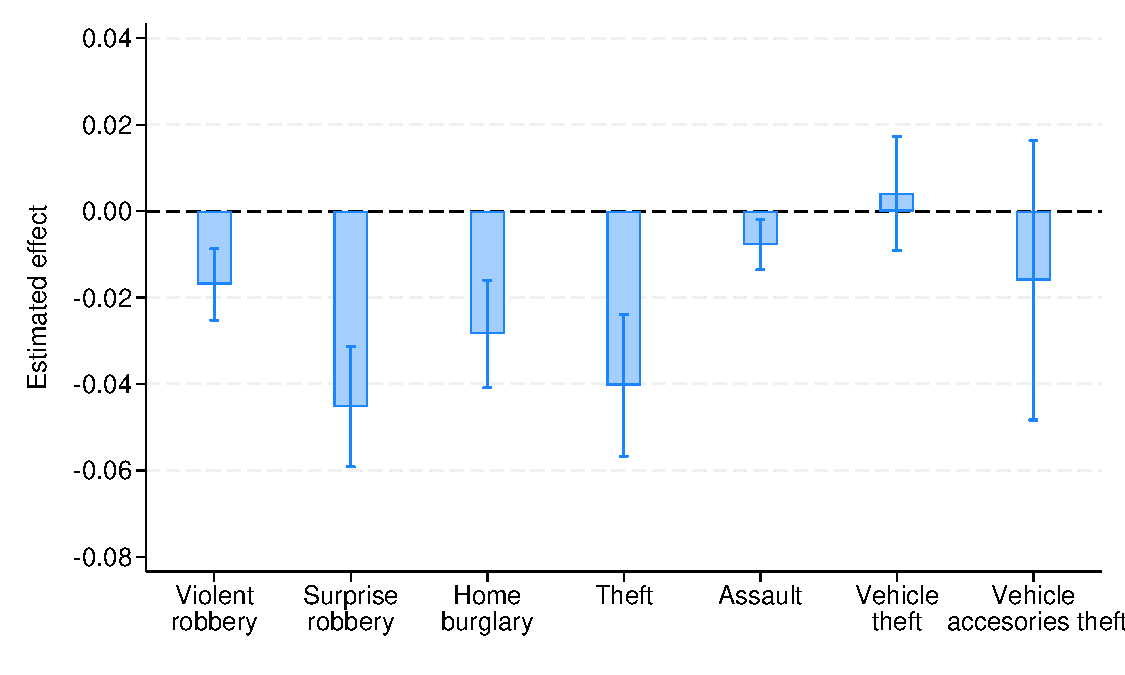
\includegraphics[width=\textwidth]{../manuscript/Graphs/results_typeofcrimes_ENUSC.pdf}
                \caption{Effects on Victimization \\ by Type of Crime}
    \end{subfigure}
    \begin{subfigure}{0.45\textwidth}
        \centering
        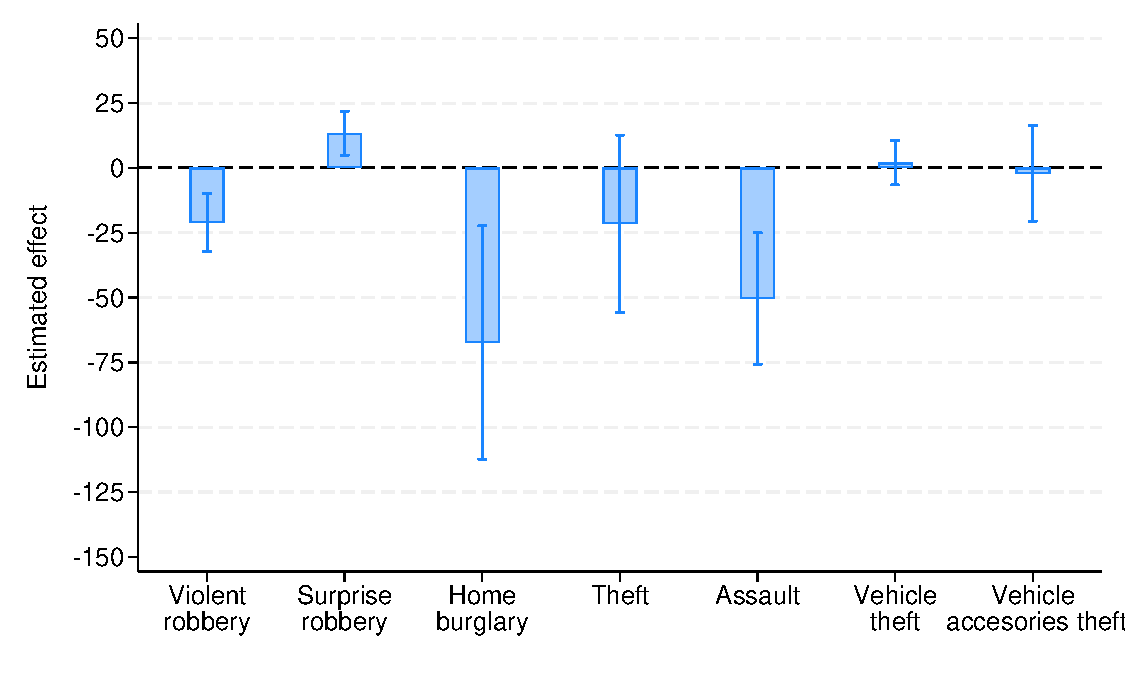
\includegraphics[width=\textwidth]{../manuscript/Graphs/results_typeofcrimes_SPD.pdf}
                \caption{Effects on Reported crime  \\ by Type of Crime}
    \end{subfigure}
    \\[12pt]
    \begin{minipage}{0.99\textwidth}
    \footnotesize Notes: This figure shows the pooled effects of the \emph{Plan Cuadrante} on victimization and number of crimes reported to the police per 100,000 inhabitants by type of crime. The estimation is conducted using the procedure developed in \citet{Callaway} for difference-in-differences with staggered treatment adoption. The graphs display the estimated coefficients and 95\% confidence intervals. Standard errors are clustered at the municipality level using the wild bootstrapping procedure.
    Panel (a) presents the results using victimization data from ENUSC surveys while Panel (b) presents the results using municipality-level administrative data on crime reported to the police provided by the Undersecretary for Crime Prevention. 
    \end{minipage}
\end{figure}
\clearpage

\subsection{Effects of \emph{Plan Cuadrante} on Crime Preventing Measures by Type of Measure and Household SES}
Table \ref{tab:hhprotectionmeasurestype} presents the effect of \emph{Plan Cuadrante} on different types of crime prevention measures by the socioeconomic status of households. The results indicate that \emph{Plan Cuadrante} reduces household investments in crime prevention measures across all socioeconomic groups, particularly investments in more affordable measures such as grilles and dogs.

\begin{table}[h!]
\caption{Effects of \emph{Plan Cuadrante} on Household Security Measures, by Type of Measure and Socioeconomic Status}
\label{tab:hhprotectionmeasurestype}
\begin{center}
\resizebox{\textwidth}{!}{
\begin{tabular}{lcccccc} \hline \hline
& (1) & (2) & (3) & (4) & (5) & (6) \\
& \multicolumn{3}{c}{Cheap measures} & \multicolumn{3}{c}{Expensive measures} \\
\cmidrule(lr){2-4} \cmidrule(lr){5-7}
& All & Higher SES & Lower SES & All & Higher SES & Lower SES \\
\cmidrule(lr){2-4} \cmidrule(lr){5-7}
\\
ATT & -0.072*** & -0.090*** & -0.058*** & -0.015*** & -0.028*** & -0.004 \\
& (0.015) & (0.018) & (0.018) & (0.005) & (0.010) & (0.005) \\
\\
N & 93,041 & 40,377 & 52,664 & 93,041 & 40,377 & 52,664 \\
Municipalities & 47 & 47 & 47 & 47 & 47 & 47 \\
Y mean & 0.176 & 0.211 & 0.151 & 0.050 & 0.085 & 0.026 \\
\hline \hline
\end{tabular}}
\par{
\begin{tabular}{p{\textwidth}}
\footnotesize{Note: This table reports the effect of \emph{Plan Cuadrante} on the probability that a household adopted a given type of security measure in the previous 12 months, using ENUSC survey data. Cheap measures are window grilles and guard dogs; expensive measures are firearms, alarms, private security insurance, and private guards. Columns (1)--(3) report the effects on cheap measures and columns (4)--(6) on expensive measures, for all households and split by household socioeconomic status (SES), with Higher SES denoting the upper SES strata and Lower SES the lower strata. The reported ATT is the average post-treatment effect, estimated with the staggered difference-in-differences procedure of \citet{Callaway}. Standard errors, clustered at the municipality level using the wild bootstrap, are reported in parentheses. The Y mean row reports the mean of the outcome among treated municipalities before adoption. ***p$<$0.01, **p$<$0.05, *p$<$0.1.} \\
\end{tabular}}
\end{center}
\end{table}

\clearpage

\subsection{Effects of \emph{Plan Cuadrante} and Changes in Police Resources}
\label{resources_plan_cuadrante} 

To make the implementation of \emph{Plan Cuadrante} possible, police resources were augmented in some municipalities. To examine the extent to which the observed results might be driven by the increase in police resources rather than by the geographic specialization component of the reform, we conduct the following two empirical exercises.

Firstly, we examine the heterogeneity of \emph{Plan Cuadrante}'s effects by the magnitude of resource increases in each municipality. Panels (a) and (b) of Figure \ref{fig:figure_resources} show that municipalities in the bottom 40\% of the resource-increase distribution---represented by blue bars---experienced increases close to the average annual variation experienced by never treated or municipalities that had not yet adopted the program (green bar), while municipalities in the top 40\% (red bars) experienced larger increases, with officers rising by around 22\% and patrol vehicles by around 80\%. If the effects of \emph{Plan Cuadrante} were driven by resource increases alone, we would not expect to see any effect in municipalities with increases in police resources similar in magnitude to those observed in the control group. To conduct our heterogeneity analysis, we split the sample into municipalities with small and large resource increases and estimate specification (\ref{eq:main}) separately for each subsample. Yet panels (c) and (d) of Figure \ref{fig:figure_resources} show that the effects on most outcomes remain sizeable for most crime and crime perception outcomes even among municipalities with resource increases similar to the control group. While there might be a resource gradient for the effects on crime perception, the effects on twelve-month victimization and private investment in security, in municipalities with resource increases similar to those in the control group, are comparable in magnitude to the effects among municipalities with larger resource increases. The effect on the probability of complaining about police surveillance, arguably a proxy for police presence, was also similar for both groups.\footnote{We provide the heterogeneous effects of \emph{Plan Cuadrante} on complaints about lack of police surveillance because information on this variable is available for the period 2003-2012. However, information on the share of households perceiving an increase in police presence, reporting that police passed by their house daily and never seeing police patrols near their house is only available in ENUSC rounds 2003, 2005 and 2006, and therefore there is not sufficient overlap with information on resources, available from 2005 for patrol vehicles and from 2006 for police officers.} More generally, we cannot reject the hypothesis that effects are equal between the two groups in all the examined outcomes. The heterogeneous effects on trust in the police, complaints about the lack of police officers, and arrests---the three outcomes not shown in Figure \ref{fig:figure_resources}---are reported in Figure \ref{fig:heterogeneity_appendix} and are likewise similar across the two groups.

\FloatBarrier
\begin{figure}[h!]
    \centering
    \caption{Effects of \emph{Plan Cuadrante} by Resource Increase: Trust, Complaints, and Arrests}
    \label{fig:heterogeneity_appendix}
    \begin{subfigure}[t]{0.48\textwidth}
        \centering
        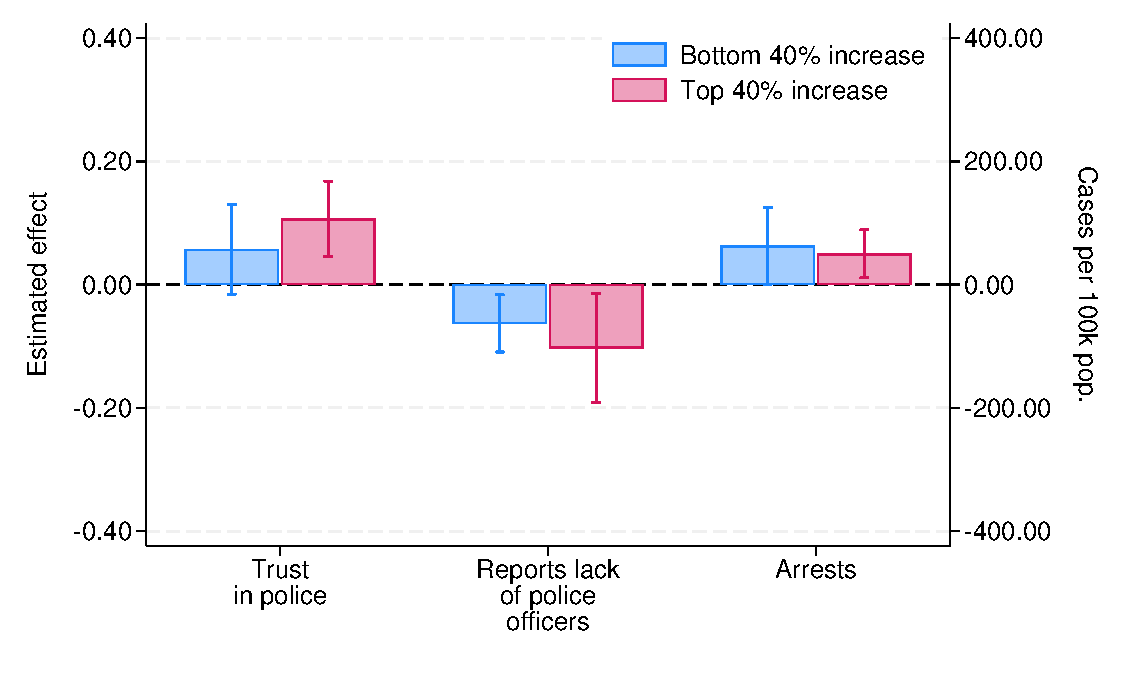
\includegraphics[width=\linewidth]{../manuscript/Graphs/heterogeneity_off_appendix.pdf}
        \caption{By the intensity of $\Delta$ in police officers}
    \end{subfigure}\hfill
    \begin{subfigure}[t]{0.48\textwidth}
        \centering
        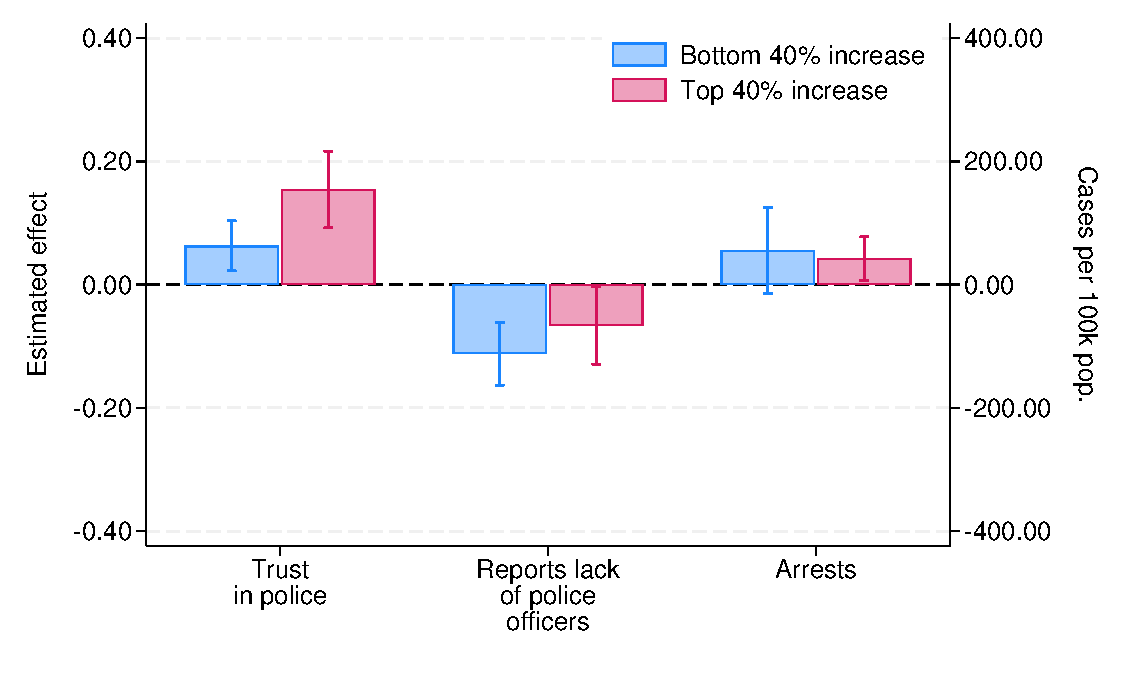
\includegraphics[width=\linewidth]{../manuscript/Graphs/heterogeneity_pv_appendix.pdf}
        \caption{By the intensity of $\Delta$ in patrol vehicles}
    \end{subfigure}
    \\[8pt]
    \begin{minipage}{0.99\textwidth}
    \footnotesize Notes: This figure complements Figure \ref{fig:figure_resources} by reporting, for the three outcomes not shown there, the effect of \emph{Plan Cuadrante} estimated separately for municipalities in the bottom 40\% (blue) and top 40\% (red) of the resource-increase distribution. Panel (a) splits municipalities by the increase in police officers and panel (b) by the increase in patrol vehicles. In each panel, arrests (administrative data, in cases per 100,000 inhabitants) are read on the right axis; the other two outcomes, from the ENUSC survey (trust in the police, and reports about the lack of police officers), are read on the left axis. Effects are estimated using the difference-in-differences estimator for staggered treatment adoption developed in \citet{Callaway}; bars are point estimates and whiskers 95\% confidence intervals, with standard errors clustered at the municipality level using the wild bootstrapping procedure.
    \end{minipage}
\end{figure}

\FloatBarrier

Finally, we re-estimate the main results of the study reported in Figure \ref{fig:figure02}, controlling for the number of police officers and the number of patrol vehicles in the municipality.

The results of this analysis are reported in Table \ref{tab:results_controlbyresources}. The magnitude of the estimated effects remains similar for most variables, although the statistical significance is reduced in some estimations. This likely reflects a mechanical feature of the \citet{Callaway} estimation procedure: control variables are not incorporated parametrically, but are instead used to construct the comparison group via outcome regression or propensity-score weighting, so the resulting estimation uncertainty propagates to the ATT standard errors. Note, however, that these resource variables are bad controls, as they are affected by the adoption of \emph{Plan Cuadrante}, so these results should be interpreted with caution.


\begin{table}[h!]\centering
\caption{Effects of \emph{Plan Cuadrante} Controlling for Police Resources}
\label{tab:results_controlbyresources}
\resizebox{\textwidth}{!}{
\begin{threeparttable}
\begin{tabular}{l ccccc}
\toprule
 & (1) & (2) & (3) & (4) & (5) \\
\midrule
\multicolumn{6}{l}{\textit{Panel A. Victimization}} \\[0.2em]
ATT &       -0.099*** &       -0.077*** &       -0.086** &       -0.094*** &       -0.087* \\
  & (0.013) & (0.013) & (0.043) & (0.028) & (0.053) \\
N &    93,041 &    53,973 &    53,553 &    72,017 &    53,553 \\[0.4em]
\multicolumn{6}{l}{\textit{Panel B. Crime perception}} \\[0.2em]
ATT &       -0.149*** &       -0.140*** &       -0.112** &       -0.082** &       -0.111 \\
  & (0.025) & (0.032) & (0.057) & (0.033) & (0.106) \\
N &    89,578 &    52,160 &    51,746 &    69,434 &    51,746 \\[0.4em]
\multicolumn{6}{l}{\textit{Panel C. Investment in security measures}} \\[0.2em]
ATT &       -0.077*** &       -0.066*** &       -0.109*** &       -0.081*** &       -0.168*** \\
  & (0.016) & (0.019) & (0.041) & (0.019) & (0.064) \\
N &    93,041 &    53,973 &    53,553 &    72,017 &    53,553 \\[0.4em]
\multicolumn{6}{l}{\textit{Panel D. Reported crime (per 100k pop.)}} \\[0.2em]
ATT &     -208.024*** &     -190.446*** &       29.230 &     -261.439 &     -245.555 \\
  & (56.130) & (67.908) & (147.261) & (170.954) & (165.221) \\
N &     4,231 &     1,918 &     1,911 &     2,248 &     1,911 \\[0.4em]
\midrule
Sample                   & Full & Resource yrs & Resource yrs & Resource yrs & Resource yrs \\
Police officers (per 100k pop.) &      &            & \checkmark &            & \checkmark \\
Patrol vehicles (per 100k pop.) &      &            &            & \checkmark & \checkmark \\
\bottomrule
\end{tabular}
\begin{tablenotes}[flushleft]
\item \footnotesize{Note: ATT estimates of the effect of \emph{Plan Cuadrante} on each outcome. Column (1) is the baseline (full estimation sample, no controls) and reproduces the headline estimate of the corresponding estimator. Column (2) restricts the estimation to 2006--2012, the window over which police resources are observed, without including any control variable. Columns (3)--(5) add time-varying controls for police resources per 100{,}000 inhabitants: officers only; patrol vehicles only; and officers and patrol vehicles jointly (entered as separate regressors). Columns (3) and (5) cover 2006--2012, the years for which the number of officers is observed; column (4) also includes 2005, the first year for which patrol vehicles are observed. Patrol vehicles are measured, per 100{,}000 inhabitants, as all patrol automobiles (radiopatrulla, auto patrullero, auto policial, automovil, station wagon, jeep and camioneta) plus motorcycles. Standard errors in parentheses; row N reports the estimation-sample size. Estimation follows \citet{Callaway}; standard errors clustered at the municipality level using wild bootstrapping procedures. $^{*}p<0.1$, $^{**}p<0.05$, $^{***}p<0.01$.}
\end{tablenotes}
\end{threeparttable}}
\end{table}


\clearpage

\subsection{Factors Associated with the Increase in Police Resources}
\label{sec:resource_correlates}

As discussed in Section \ref{institutions} and in Online Appendix \ref{resources_plan_cuadrante}, the increase in police resources associated with the adoption of \emph{Plan Cuadrante} varied substantially across municipalities. In principle, this increase should be related to each municipality's pre-existing police resource deficit---measured in Equivalent Surveillance Units (UVEs)---which \emph{Plan Cuadrante} was meant to help close. However, program evaluations do not clearly establish that this deficit is what determined the size of the resource increase each municipality received \citep{DIPRES2007_largo,DIPRES2014}.\footnote{Although we requested information on the demand and supply of UVEs underlying this allocation, this information was not provided by \textit{Carabineros}.} If the pre-existing deficit is not what determines the resource increase, what is it related to? Reassuringly, municipalities receiving larger versus smaller resource increases do not display differential pre-treatment trends in either the outcomes of interest or in police resources themselves.\footnote{We test for the joint significance of the pre-treatment coefficients between the two groups, separately for the split based on the increase in police officers and the split based on the increase in patrol vehicles. The resulting p-values are, respectively, 0.823 and 0.048 for victimization, 0.059 and 0.379 for crime perception, 0.820 and 0.157 for investment in security measures, and 0.213 and 0.419 for reported crime, as well as 0.616 and 0.444 for police officers and 0.405 and 0.157 for patrol vehicles.} In this section we examine whether the magnitude of the resource increase experienced by a municipality upon adoption is correlated with its pre-treatment levels in crime, police resources, and other observable characteristics. Specifically, we regress the increase in resources at the time of adopting \emph{Plan Cuadrante} on municipality characteristics measured before the program's introduction, including crime and police resources in 2006, the first year for which information on police resources is available. Thus, we restrict this analysis to municipalities that adopted \emph{Plan Cuadrante} from 2007 onward.

Table \ref{tab:resourcecorrelates} reports OLS regressions of the average annual increase in police officers and patrol vehicles per 100,000 inhabitants on pre-adoption municipality characteristics, separately for the administrative (SPD) sample at the municipality level (columns 1--2) and the ENUSC sample at the survey-respondent level (columns 3--4). All variables are standardized and standard errors are clustered by municipality, so coefficients are comparable in magnitude across regressors.

The results provide little support for the hypothesis that municipalities with worse pre-treatment crime outcomes received systematically larger resource increases. Pre-treatment reported crime is, if anything, negatively associated with the subsequent increase in both officers and vehicles in the administrative sample (columns 1--2); in the ENUSC sample, it is negatively associated with the increase in officers (column 3), although it is positively associated with the increase in vehicles (column 4). Pre-treatment victimization is, if anything, negatively associated with both increases in the ENUSC sample (columns 3--4). Pre-treatment arrests, crime perception, trust in the police, and private investment in security measures are not significantly associated with the resource increase. The increase in resources is instead more strongly predicted by structural municipality characteristics: less populous municipalities experienced larger increases in three of the four specifications, and municipalities with higher poverty rates predicted a larger increase in vehicles in the administrative sample (column 2), although this association is not significant for officers in that sample (column 1) or in the ENUSC sample (columns 3--4).

\begin{table}[H]
\centering
\caption{Predictors of the Increase in Police Resources under \emph{Plan Cuadrante}}
\label{tab:resourcecorrelates}
\begin{threeparttable}
\small
\setlength{\tabcolsep}{6pt}
\renewcommand{\arraystretch}{1.1}
\begin{tabular}{@{}l cc cc@{}}
\toprule
& \multicolumn{2}{c}{Administrative sample} & \multicolumn{2}{c}{ENUSC sample} \\
\cmidrule(lr){2-3} \cmidrule(lr){4-5}
& Police & Patrol & Police & Patrol \\
Dep.\ var: avg.\ annual increase & officers & vehicles & officers & vehicles \\
in resources (share of pre-adoption level) & (1) & (2) & (3) & (4) \\
\midrule
Reported crime (per 100k pop.) & $-0.203^{**}$ & $-0.199^{**}$ & $-0.319^{*}$ & $0.272^{*}$ \\
 & (0.099) & (0.097) & (0.182) & (0.137) \\
Arrests (per 100k pop.) & $0.099$ & $-0.041$ & $0.003$ & $0.297$ \\
 & (0.136) & (0.129) & (0.186) & (0.223) \\
Victimization &  &  & $-0.017^{*}$ & $-0.025^{*}$ \\
 &  &  & (0.010) & (0.013) \\
Crime perception &  &  & $0.005$ & $0.008$ \\
 &  &  & (0.017) & (0.014) \\
Trust in the police &  &  & $0.024$ & $0.027$ \\
 &  &  & (0.018) & (0.019) \\
Investment in security measures &  &  & $0.004$ & $-0.003$ \\
 &  &  & (0.010) & (0.009) \\
Police officers (per 100k pop.) & $-0.207$ & $0.155$ & $-0.888^{***}$ & $0.571^{***}$ \\
 & (0.155) & (0.129) & (0.154) & (0.136) \\
Patrol vehicles (per 100k pop.) & $-0.129$ & $-0.139$ & $0.537^{**}$ & $-0.507^{***}$ \\
 & (0.129) & (0.126) & (0.212) & (0.169) \\
Log population & $-0.529^{***}$ & $-0.203^{*}$ & $-0.193$ & $-0.626^{**}$ \\
 & (0.145) & (0.112) & (0.189) & (0.269) \\
Poverty rate (2004) & $0.170$ & $0.308^{**}$ & $0.027$ & $-0.017$ \\
 & (0.113) & (0.126) & (0.108) & (0.108) \\
\midrule
Observations & 65 & 65 & 8,781 & 8,781 \\
R-squared & 0.342 & 0.282 & 0.614 & 0.545 \\
\bottomrule
\end{tabular}
\begin{tablenotes}[flushleft]
\footnotesize
\item \textit{Note:} OLS regressions of the average annual increase in police officers (columns 1 and 3) and patrol vehicles (columns 2 and 4) per 100{,}000 inhabitants, from the year before adoption of \emph{Plan Cuadrante} to 2012. As in panels (a) and (b) of Figure \ref{fig:figure_resources}, the increase is expressed as a share of the resources available the year before adoption. Columns 1--2 use the administrative sample at the municipality level; columns 3--4 use ENUSC survey respondents interviewed before 2007 (survey outcomes at the respondent level, other regressors as pre-2006 municipality aggregates). All variables are standardized. Standard errors clustered by municipality in parentheses.
\item $^{*}p<0.1$; $^{**}p<0.05$; $^{***}p<0.01$.
\end{tablenotes}
\end{threeparttable}
\end{table}


\clearpage

\subsection{Police Resources and Police Effectiveness}
\label{resources_vs_specialization}

This Online Appendix presents two additional empirical analyses examining the link between police resources and crime in Chile, outside the scope of \emph{Plan Cuadrante}.

First, we assess the effects of \textit{Seguridad Ciudadana}, a program that creates a security force that, while they do not have the competence to apprehend or carry weapons, assist Carabineros in their work, effectively increasing their human resources for tasks such as patrolling and other deterrence activities. Like \emph{Plan Cuadrante}, the creation of these municipal security forces was staggered and started after 2012 in nearly all municipalities.\footnote{Among the municipalities in the ENUSC survey, only Curic\'o introduced the \textit{Seguridad Ciudadana} program before 2013, being 2012 the last year in which \emph{Plan Cuadrante} was implemented for the first time in a municipality surveyed in ENUSC. Among the full set of 346 municipalities, only 10 of them introduced the program \textit{Seguridad Ciudadana} before 2013, all of them except Curic\'o being small municipalities.} We hand-collected the year in which each municipality established its \textit{Seguridad Ciudadana} program, requesting this information from all 346 Chilean municipalities through the national transparency portal (\emph{Portal de Transparencia}) and compiling the responses they returned into an original dataset. Using administrative and ENUSC data available until 2017, the estimated effects of \textit{Seguridad Ciudadana} program are presented in Figure \ref{fig:figureA5}. We estimate the effects for all the outcomes examined in the \emph{Plan Cuadrante} analysis except for trust in the police, since information on the latter variable is rarely collected in ENUSC rounds conducted after 2012. The results show that this program had little effects on every dimension of police effectiveness considered. This result is also consistent with the hypothesis that the large effects of \emph{Plan Cuadrante} on police effectiveness are unlikely driven entirely by the change in police resources brought by the program.

\begin{figure}[h!]
    \centering
    \caption{Effects of \textit{Seguridad Ciudadana} on Crime Outcomes and Security Perceptions}
    \label{fig:figureA5}
    
    % Primera fila: panel (a) y (b)
    \begin{subfigure}{0.495\textwidth}
        \centering
        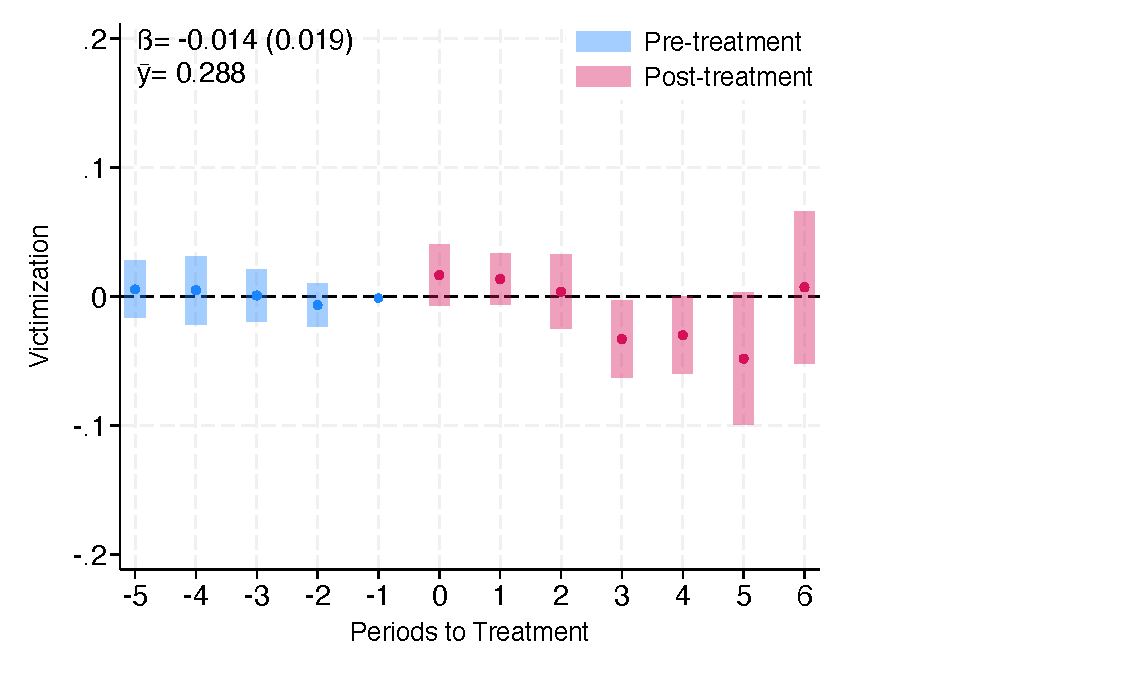
\includegraphics[width=\textwidth]{../manuscript/Graphs/results_victimization_SC.pdf}
        \caption{Victimization in last 12 months}
    \end{subfigure}%
    \hfill
    \begin{subfigure}{0.495\textwidth}
        \centering
        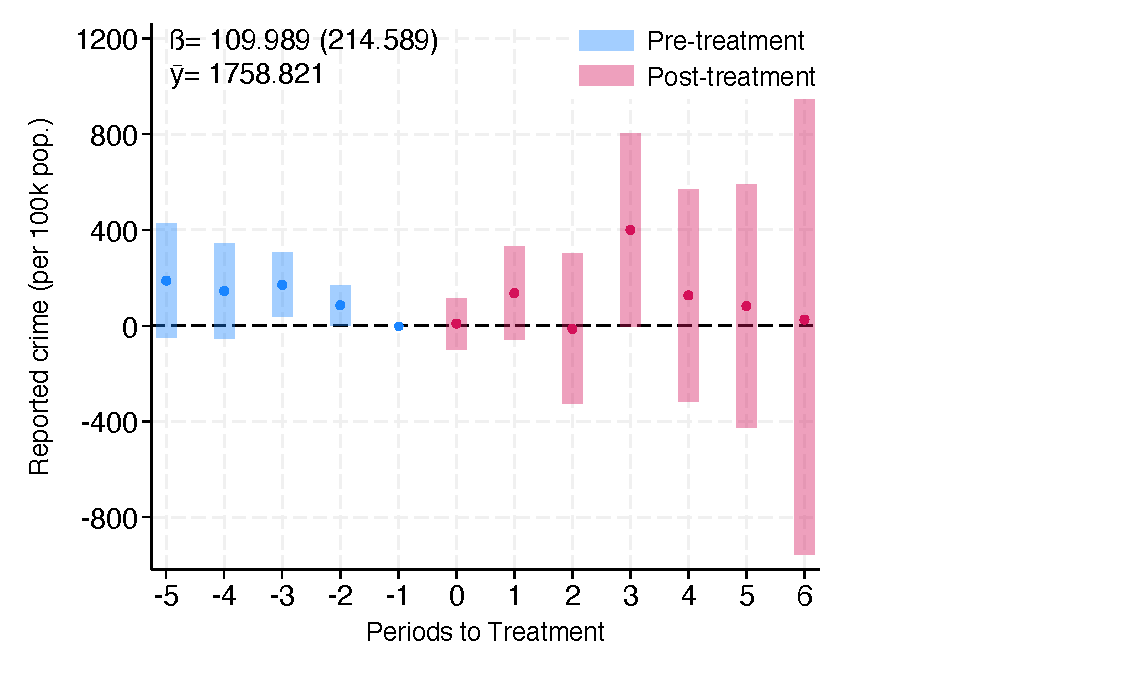
\includegraphics[width=\textwidth]{../manuscript/Graphs/totalreportedcrime_allcomunas_SC.pdf}
        \caption{Reported crime per 100k inhabitants}
    \end{subfigure}

    \vspace{12pt} % Espacio entre filas
    
    % Segunda fila: panel (c) y (d)
    \begin{subfigure}{0.495\textwidth}
        \centering
        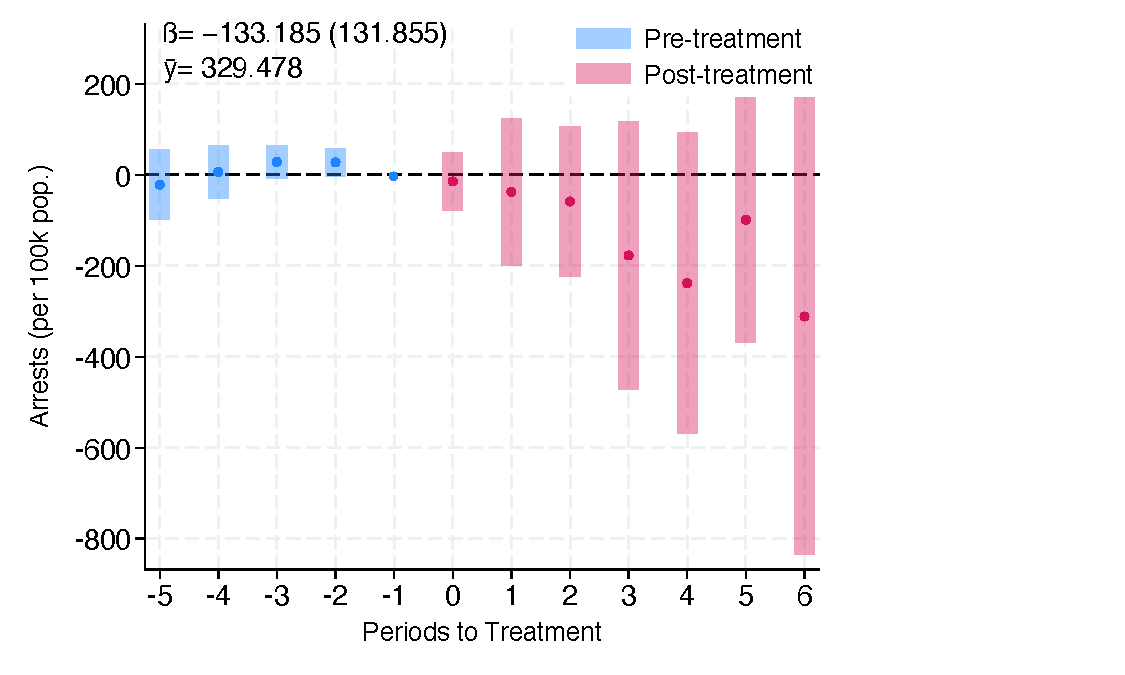
\includegraphics[width=\textwidth]{../manuscript/Graphs/totalarrestscrime_allcomunas_SC.pdf}
        \caption{Arrests per 100k inhabitants}
    \end{subfigure}%
    \hfill
    \begin{subfigure}{0.495\textwidth}
        \centering
        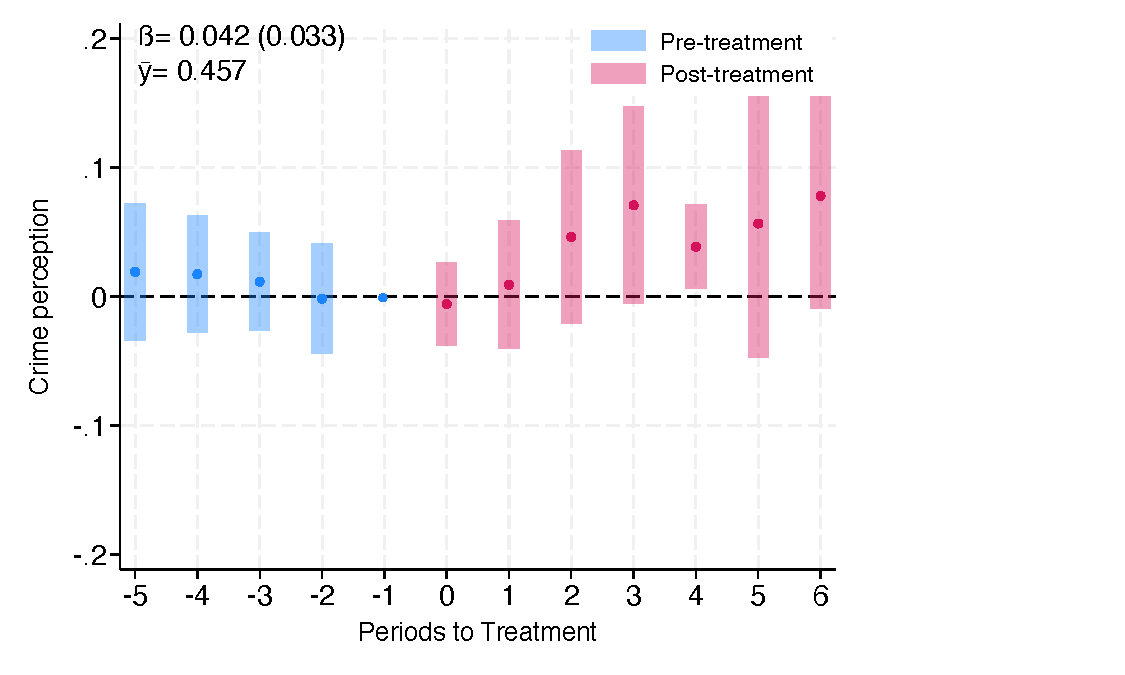
\includegraphics[width=\textwidth]{../manuscript/Graphs/results_perception_SC.pdf}
        \caption{Households reporting an \\ increase in crime}
    \end{subfigure}
    
    \vspace{12pt} % Espacio entre filas
    
    % Tercera fila: panel (e)
    \begin{subfigure}{0.495\textwidth}
        \centering
        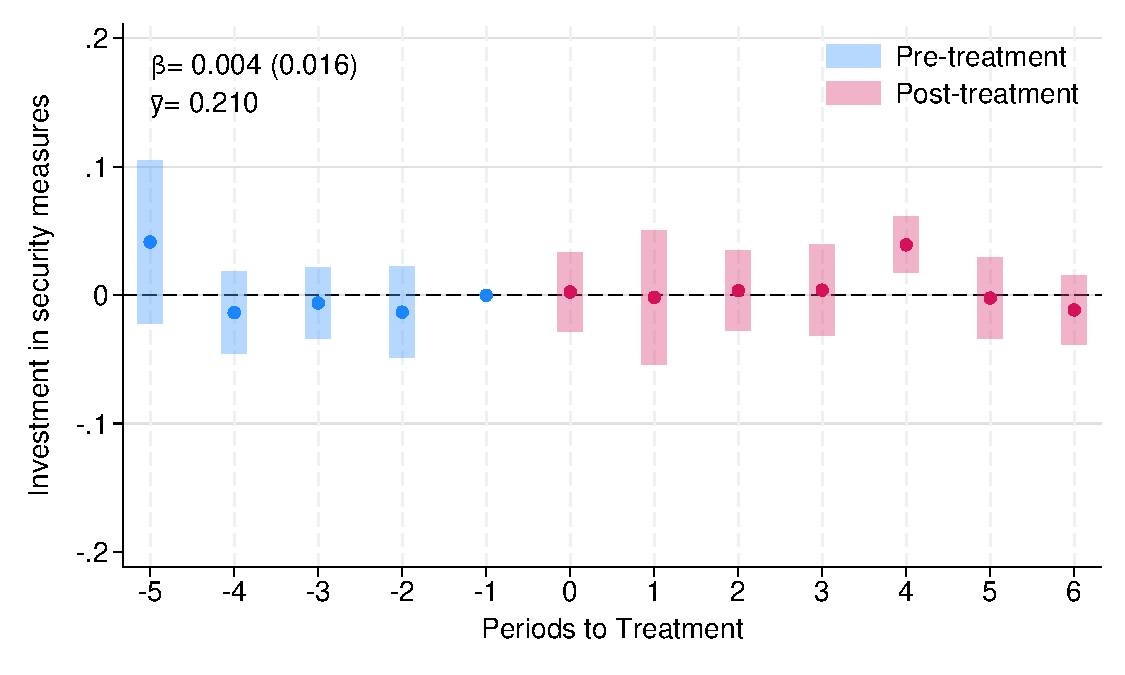
\includegraphics[width=\textwidth]{../manuscript/Graphs/results_hhprotectionmeasures_SC.pdf}
        \caption{Households adopting security measures}
    \end{subfigure}

    \vspace{12pt} % Espacio para las notas
    
    \begin{minipage}{0.99\textwidth}
        \footnotesize
        Notes: This figure shows the dynamic effects of the \textit{Seguridad Ciudadana} program on different measures of crime and security perceptions. The estimation is conducted using the procedure developed in \citet{Callaway} for difference-in-differences with staggered treatment adoption. The dots in the figure represent the estimated coefficients and the bars behind them 95\% confidence intervals. Standard errors are clustered at the municipality level using wild bootstrapping. The pooled effect and the mean outcome before the introduction of the treatment for the outcome---computed as in Figure \ref{fig:figure02}, using only the pre-treatment observations of treated units---is also presented in each panel. Panel (a) reports the effect of \textit{Seguridad Ciudadana} on the probability of household victimization in the last 12 months using the ENUSC survey. Panel (b) reports the effect on the number of crimes reported to the police in the municipality per 100,000 inhabitants using administrative data. Panel (c) reports the effect on the number of arrests in the municipality per 100,000 inhabitants using administrative data. Panel (d) reports the effect on the probability of perceiving an increase in crime using the ENUSC survey. Panel (e) reports the effect on the probability of adopting security measures in the last twelve months using the ENUSC survey. Panel (a) includes 210,102 observations; panel (b), 2,234; panel (c), 1,908; panel (d), 203,078; and panel (e), 74,316 observations.
    \end{minipage}
\end{figure}

\clearpage

Secondly, we use yearly information on the number of police officers and patrol vehicles at the municipality level facilitated by \textit{Carabineros} for the period 2006-2012 to examine the statistical association between police resources and crime, controlling for year and municipality fixed effects. Specifically, we estimate the following regression:

\begin{equation}
Crime_{imt}=  \delta_{1} \mbox{\textit{Police resources}}_{mt} +  Municipality_{m}   +      Year_{t} +  u_{imt}
\label{eq:correlation}
\end{equation}

\noindent where \textit{Police resources} indicates either the number of police officers per 100,000 inhabitants in municipality $m$ during year $t$ or the number of patrol vehicles per 100,000 inhabitants in municipality $m$ during year $t$. We focus on the 41 municipalities of Santiago surveyed in ENUSC for the period 2006-2012. The study period is delimited by the availability of data on police resources. We focus on the municipalities of Santiago because \emph{Plan Cuadrante} was implemented in all of these municipalities by 2000. Expanding the analysis to other municipalities may confound the dynamic effects of \emph{Plan Cuadrante} with the potential effects of subsequent increases in police resources. Between 2006 and 2012, these municipalities saw an average increase of 26\% in police officers and 83\% in patrol vehicles.

The results of the analyses are reported in Figure \ref{fig:figureA7B}. While the set of fixed effects account for time-invariant unobservable characteristics of the municipalities and the time shocks that affects all municipalities at the same time, the coefficients should be interpreted with caution due to potential endogeneity concerns. Overall, the results show little statistical association between police resources and the different outcomes examined, except for perceived crime. The lack of statistical association between police resources and the main outcomes is consistent with the increase of resources playing a limited role in explaining the effects of \emph{Plan Cuadrante}. Figure \ref{fig:figureA7B} reports these associations for two samples shown side by side: the 41 metropolitan municipalities of Santiago (blue bars) and the broader set of municipalities that implemented \emph{Plan Cuadrante} before 2006 together with the never treated municipalities surveyed in ENUSC (red bars). The results are similar across both samples.

\begin{figure}[h!]
    \centering
    \caption{Association between Police Resources and Police Effectiveness (No \emph{Plan Cuadrante} Variation)}
    \label{fig:figureA7B}
    \begin{subfigure}[t]{0.48\textwidth}
        \centering
        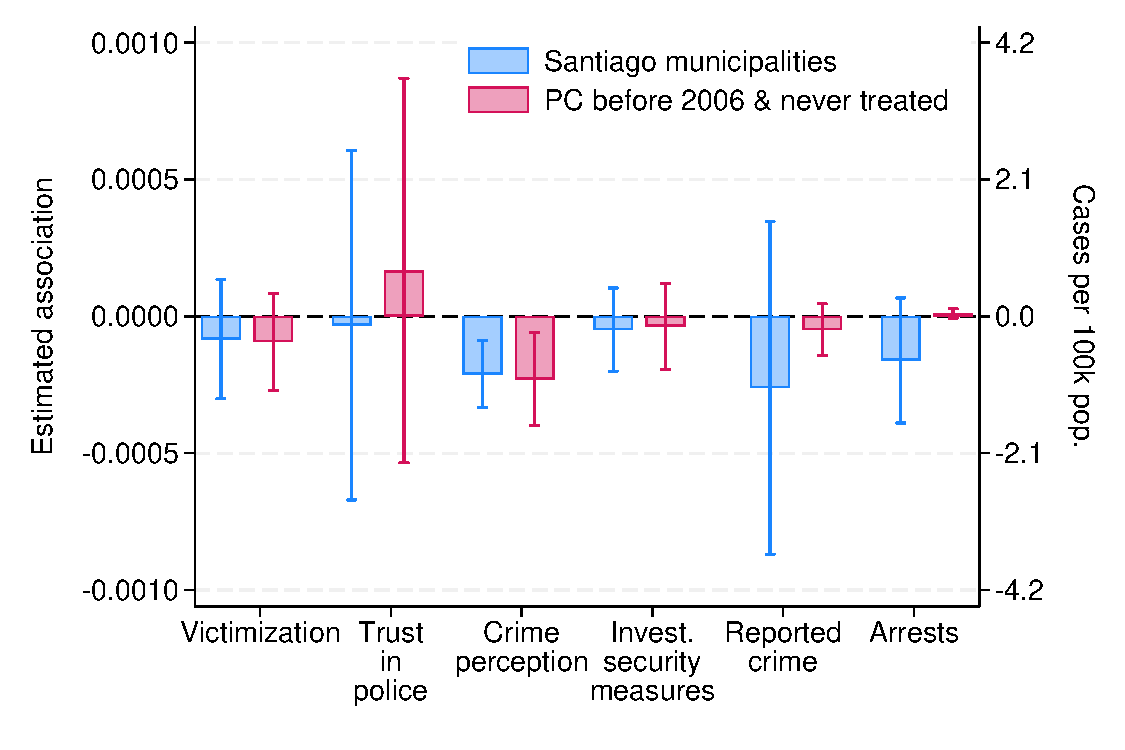
\includegraphics[width=\linewidth]{../manuscript/Graphs/results_corr_novariation_off.pdf}
        \caption{Association with police officers}
    \end{subfigure}\hfill
    \begin{subfigure}[t]{0.48\textwidth}
        \centering
        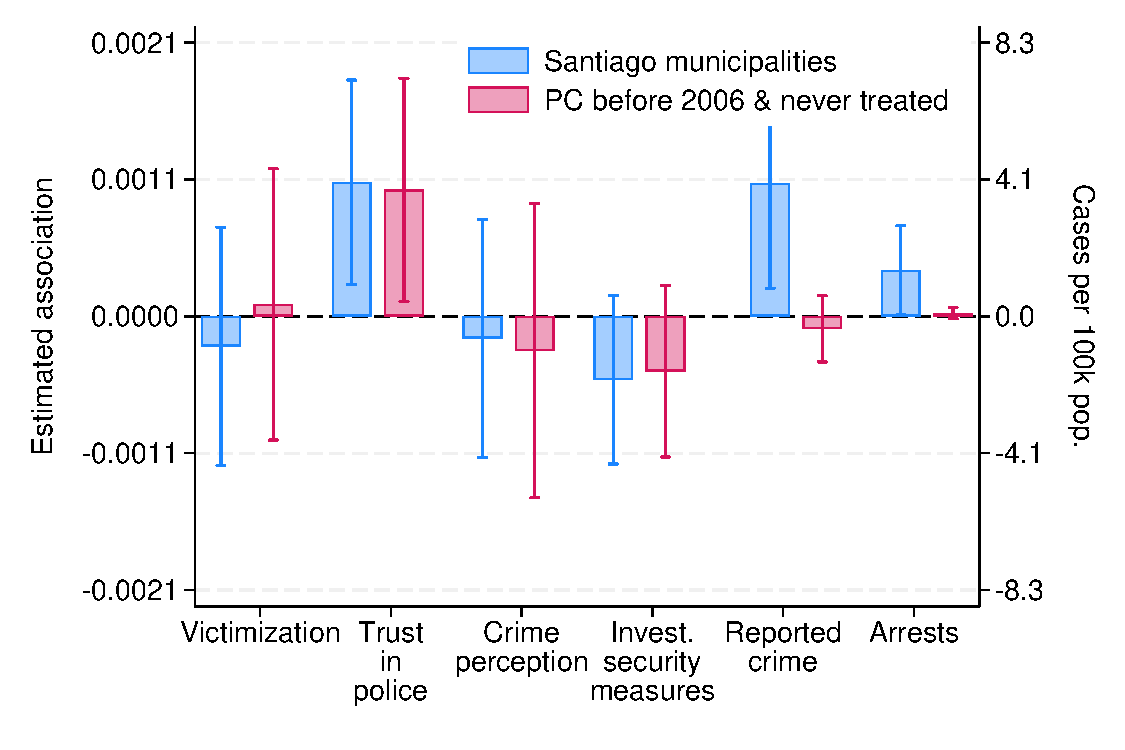
\includegraphics[width=\linewidth]{../manuscript/Graphs/results_corr_novariation_veh.pdf}
        \caption{Association with patrol vehicles}
    \end{subfigure}
    \\[10pt]
    \begin{minipage}{0.99\textwidth}
    \footnotesize Notes: The figure shows the estimated within-municipality association between police resources (per 100,000 inhabitants) and the main outcomes, in municipalities where \emph{Plan Cuadrante} does not vary over the sample period. Estimates come from OLS regressions of each outcome on the resource measure with municipality and year fixed effects; standard errors are clustered at the municipality level. Blue bars use the 41 metropolitan municipalities of Santiago, all of which adopted \emph{Plan Cuadrante} in 2000; red bars use the broader set of municipalities that adopted \emph{Plan Cuadrante} before 2006 together with the never-treated municipalities surveyed in ENUSC (2006--2012). Reported crime and arrests (administrative data, in cases per 100,000 inhabitants) are read on the right axis; all other outcomes, from the ENUSC survey (victimization, trust in the police, crime perception, and investment in security measures), are read on the left axis. Panel (a) reports associations with the number of police officers; panel (b) with the number of patrol vehicles. Bars are point estimates with 95\% confidence intervals.
    \end{minipage}
\end{figure}

\clearpage

\subsection{Adoption Timing and Perceived Police Performance}
\label{sec:balance_doseresponse}

Information on perceived police performance is only available in the 2005 round of ENUSC, so the comparison in Figure \ref{fig:figure05} relies on a single cross-section, comparing municipalities that had already adopted \emph{Plan Cuadrante} by 2005 (early adopters) with those that had not yet done so (late adopters). We consider seven measures of perceived police performance: the share of respondents who perceive police performance as good, and who perceive the police to be efficient, helpful, well informed, corrupt, failing to control crime, and failing to do their job well.


We start by assessing whether adoption timing is correlated with police performance. Using the sample of municipalities that introduced \emph{Plan Cuadrante} after 2005, Panel (a) of Figure \ref{fig:balance_doseresponse} examines the correlation between adoption timing and perceived police performance in 2005. The estimated coefficients are close to zero and statistically insignificant at conventional confidence levels, indicating that how soon a not-yet-treated municipality would go on to adopt the program is unrelated to its perceived police performance before treatment.

In Panel (b) of Figure \ref{fig:balance_doseresponse} we re-estimate the analysis conducted in Figure \ref{fig:figure05} but measuring years of exposure to \emph{Plan Cuadrante} in 2005 rather than simply whether they have adopted it or not. The results are qualitatively similar to those estimates reported in Figure \ref{fig:figure05}, showing strong correlations between years of exposure to \emph{Plan Cuadrante} and perceived police performance.

\begin{figure}[H]
    \centering
    \caption{Timing of Adoption of \emph{Plan Cuadrante} and Perceived Police Performance}
    \label{fig:balance_doseresponse}
    \begin{subfigure}{0.495\textwidth}
        \centering
        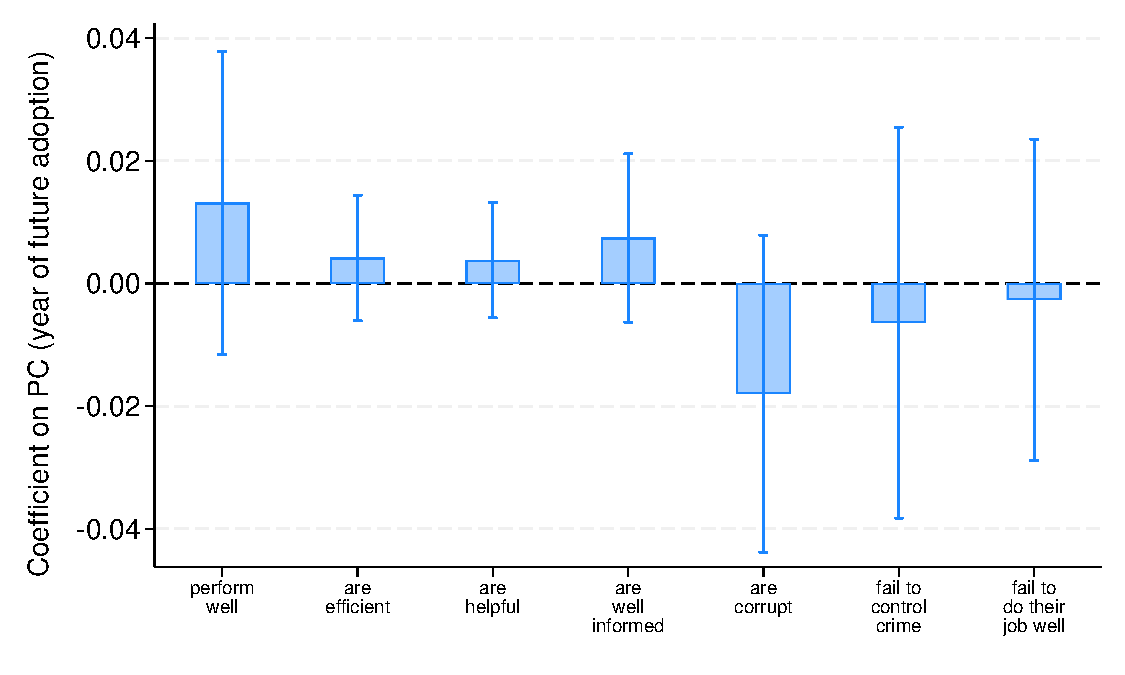
\includegraphics[width=\textwidth]{../manuscript/Graphs/balance_carabperc.pdf}
        \caption{Year of adoption and police performance before adoption}
    \end{subfigure}%
    ~
    \begin{subfigure}{0.495\textwidth}
        \centering
        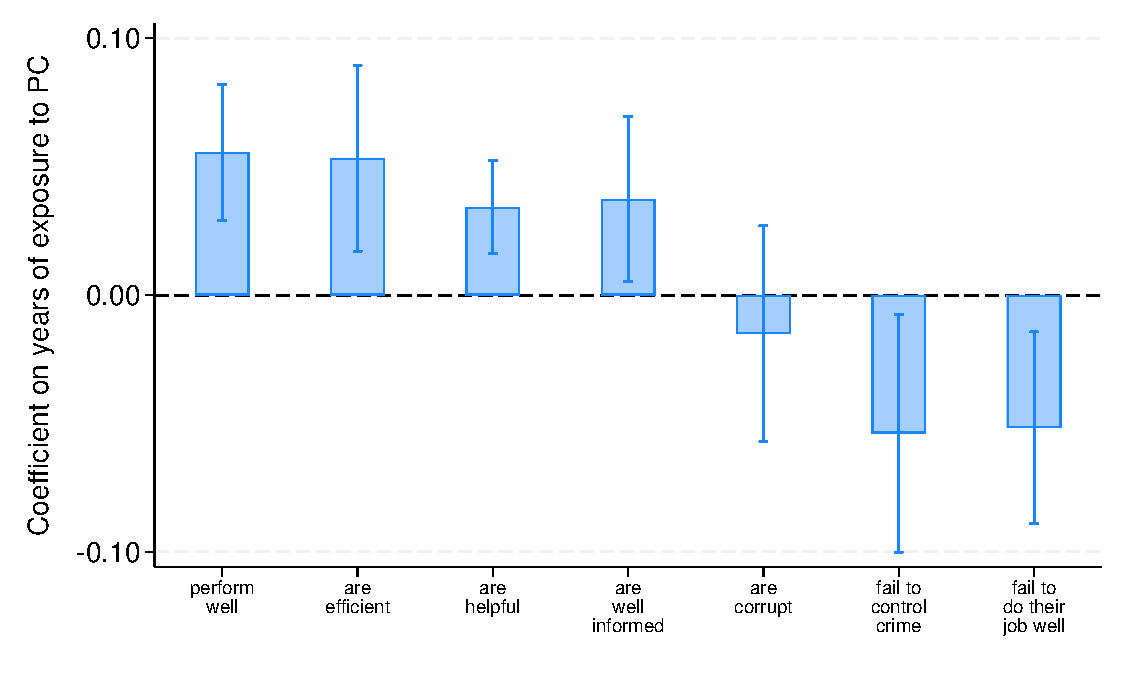
\includegraphics[width=\textwidth]{../manuscript/Graphs/doseresponse_carabperc.pdf}
        \caption{Years exposed to \emph{Plan Cuadrante} (dose response)}
    \end{subfigure}%
    \\[12pt]
    \begin{minipage}{0.99\textwidth}
    Notes: The figure considers seven measures of police performance: the share of respondents who perceive police performance as good, and who perceive the police to be efficient, helpful, well informed, corrupt, failing to control crime, and failing to do their job well. Using the sample of municipalities that adopted \emph{Plan Cuadrante} after 2005, panel (a) examines whether the future timing of adoption of \emph{Plan Cuadrante} is correlated with perceived police performance in 2005, before the introduction of the program. Panel (b) reestimates the same comparison as Figure \ref{fig:figure05}, replacing the binary adoption indicator with the municipality's number of years of exposure to \emph{Plan Cuadrante} as of 2005. In both panels, each bar plots the coefficient from a separate regression of one performance measure. The graphs display the estimated coefficients and 95\% confidence intervals.
    \end{minipage}
\end{figure}

\clearpage

%---- Online Appendix C - Robustness Checks
\clearpage

\section{Robustness Checks} \label{sec:appendixC}
\setcounter{figure}{0}
\renewcommand{\thefigure}{\Alph{section}\arabic{figure}}
\setcounter{table}{0}
\renewcommand{\thetable}{\Alph{section}\arabic{table}}

This Online Appendix presents the results of various empirical analyses that confirm the robustness of our analyses to different specifications, samples, and measures of crime. First, we show that the effects of the program on arrests and reported crimes from administrative records are not driven by the inclusion of a broader sample of municipalities in this dataset. Second, we show that our findings are robust to the use of alternative difference-in-differences estimators for staggered treatment adoption. Third, we show that the estimates presented in the main body of the paper are very similar to the ones we obtain using a balanced panel of municipalities. Fourth, we show that the results for reported crime and arrests are very similar when we use the full set of post-treatment and pre-treatment periods instead of capping the event study for symmetry with the ENUSC-based analysis. Fifth, we show that our main results remain statistically significant after applying a Bonferroni correction for multiple hypothesis testing. Sixth, we show that the results are not driven by broader temporal trends unrelated to police presence, using a placebo test based on non-neighborhood crime. Seventh, we establish that the effects of the program on crime perception remain consistent when alternative measures of crime perception available in the dataset are used. Eighth, we show that our results are robust to excluding municipalities most affected by the 2010 Maule earthquake. Finally, we document that \emph{Plan Cuadrante} has limited effects on neighboring municipalities, making it unlikely that the program’s impact on crime victimization is biased due to crime displacement.

\subsection{Effects of \emph{Plan Cuadrante} Using Administrative Data and the Sample of Municipalities Included in the ENUSC Survey}

The results reported in panel (b) of Figure \ref{fig:figure02} and in panel (a) of Figure \ref{fig:effectiveness_es} in the main manuscript show the effects of \emph{Plan Cuadrante} on the number of reported crimes in the municipality and the total number of arrests, which are administrative data provided by the police for all Chilean municipalities. The latter analysis is conducted with all never treated municipalities and municipalities that implemented the program between 2003 and 2013. This is a different analytical sample from the one used in the analysis of ENUSC survey outcomes -victimization, trust in the police, crime perception, and crime prevention measures- since the ENUSC survey was conducted only on a subsample of municipalities and for a different time period.

In this Online Appendix, we estimate the effects of \emph{Plan Cuadrante} on the number of crimes reported to the police and on the total number of arrests, using only the subsample of municipalities included in the analysis of the ENUSC outcomes. The sample size in this analysis is smaller, and the results are reported in Figure \ref{fig:figure02_N47}. While the effects for reported crime are larger in magnitude, the estimates are qualitatively similar to those observed in Table \ref{tab:SPD_all_vs_enusc} with the full sample. The estimated effect on arrests, however, is not statistically significant in this smaller ENUSC subsample, likely reflecting reduced power given the smaller number of municipalities and observations.




\begin{table}[h!]
\caption{Effects of \emph{Plan Cuadrante} on Reported Crime and Arrests: Full Sample and ENUSC Municipalities}
\label{tab:SPD_all_vs_enusc}
\begin{center}
\resizebox{12cm}{!}{
\begin{tabular}{lccccccccccccccccccccccccccccccccccccccc} \hline \hline
& & (1) & (2) & (3) & (4) \\
Outcome & & \multicolumn{2}{c}{Reported crime} & \multicolumn{2}{c}{Arrests} \\
\cmidrule(lr){3-4} \cmidrule(lr){5-6}
& & \shortstack{Sample\\Admin} & \shortstack{Sample\\ENUSC} & \shortstack{Sample\\Admin} & \shortstack{Sample\\ENUSC} \\
\cmidrule(lr){3-4} \cmidrule(lr){5-6}
\\
ATT & & -208.02*** & -428.09*** & 48.02*** & 44.09 \\
& & (56.13) & (108.48) & (16.27) & (34.85) \\
\\
N & & 4,231 & 592 & 3,293 & 405 \\
Municipalities & & 292 & 47 & 281 & 40 \\
Y mean & & 2,109.64 & 2,294.96 & 345.65 & 419.61 \\
\hline \hline
\end{tabular}}
\par{
\begin{tabular}{p{12cm}}
\footnotesize{Note: This table shows the effects of \emph{Plan Cuadrante} on the number of crimes reported to the police in the municipality per 100,000 inhabitants and on the number of arrests in the municipality per 100,000 inhabitants using administrative data from the Undersecretary for Crime Prevention. The table reports the results for two samples: the full sample of municipalities included in the administrative database that is used for the analysis of these outcomes and the subsample of these municipalities included in the analysis of ENUSC outcomes. The estimation is conducted using the procedure developed in \citet{Callaway} for difference-in-differences with staggered treatment adoption. Standard errors are clustered at the municipality level using the wild bootstrapping procedure. ***p$<$0.01, **p$<$0.05, *p$<$0.1.} \\
\end{tabular}}
\end{center}
\end{table}

\clearpage
%--- Implementation
\begin{figure}[h!]
    \centering
    \caption{Effects of \emph{Plan Cuadrante} on Reported Crime and Arrests (Sample of Municipalities Included in the Analysis of ENUSC Outcomes)}
    \label{fig:figure02_N47}
    \begin{subfigure}{0.495\textwidth}
        \centering
        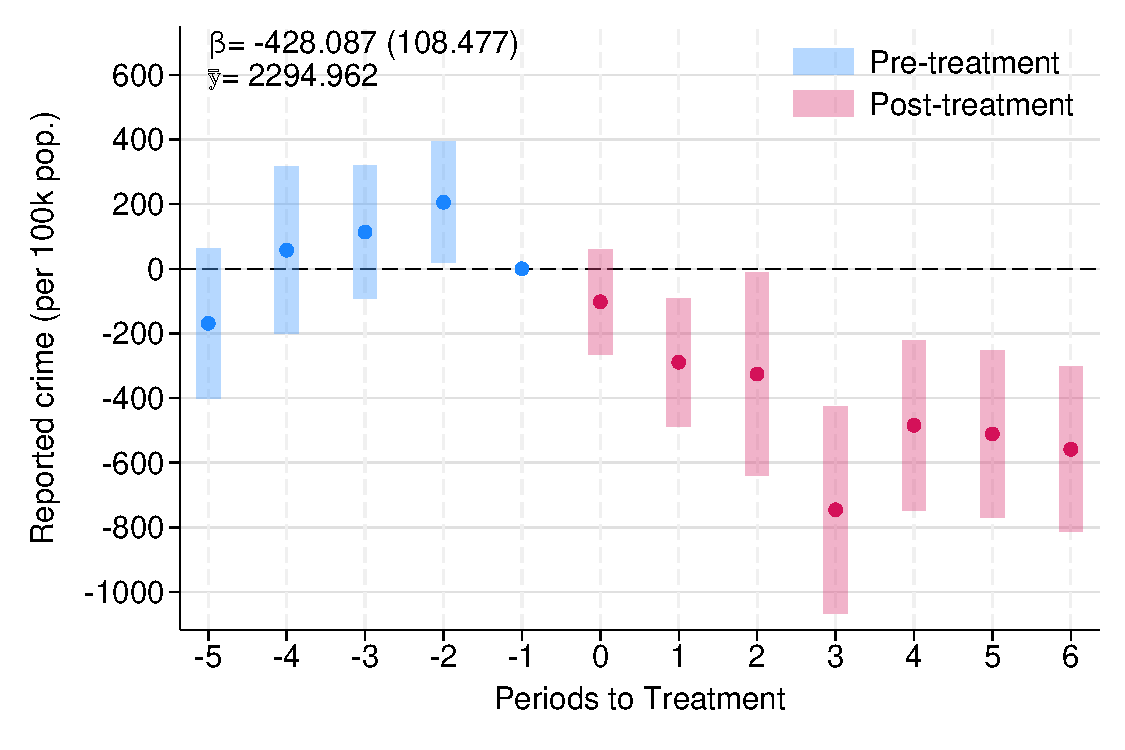
\includegraphics[width=\textwidth]{../manuscript/Graphs/totalreportedcrime_47enusc.pdf}
        \caption{Reported crime per 100k inhabitants}
    \end{subfigure}%
    ~ 
    \begin{subfigure}{0.495\textwidth}
    \centering
    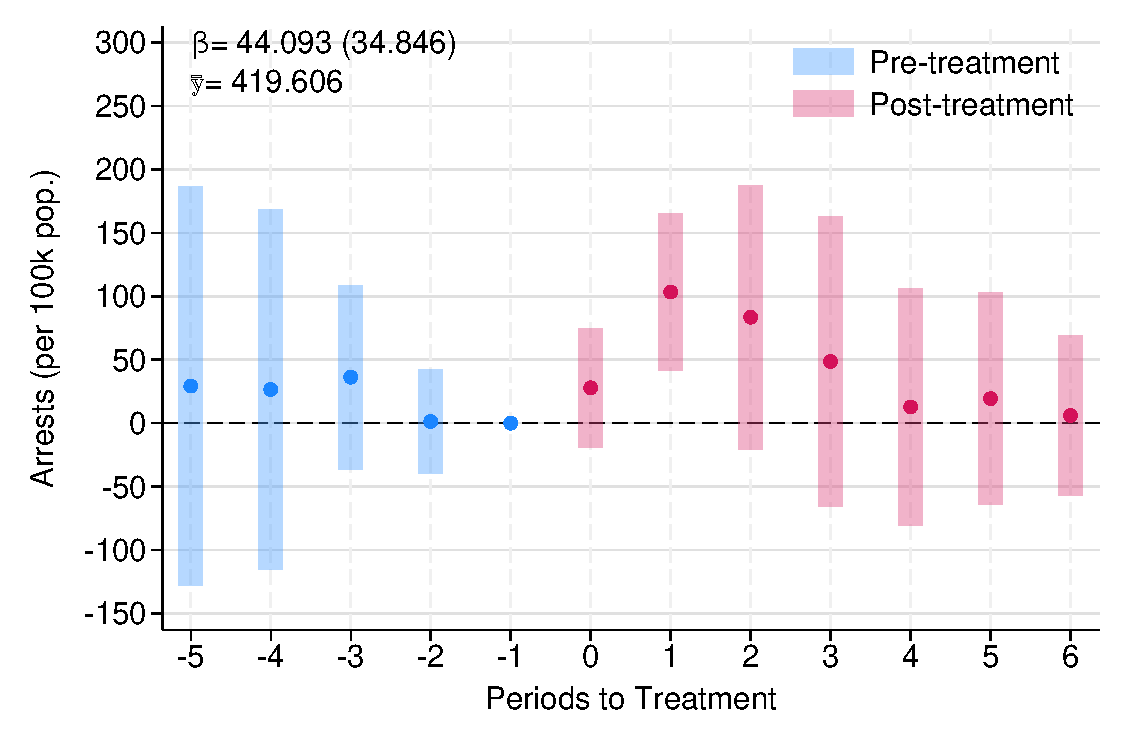
\includegraphics[width=\textwidth]{../manuscript/Graphs/totalarrestscrime_47enusc.pdf}
        \caption{Arrests per 100k inhabitants}
    \end{subfigure}
    \\[12pt]
    \begin{minipage}{0.99\textwidth}
    \footnotesize Notes: This figure shows the dynamic effects of \emph{Plan Cuadrante} on the number of crimes reported to the police per 100,000 inhabitants in the municipality in panel (a) and on the number of arrests per 100,000 inhabitants in the municipality in panel (b) using administrative data from the Undersecretary for Crime Prevention. The analysis is conducted using only the sample of municipalities included in the analysis of ENUSC outcomes. Panel (a) includes 592 observations, while panel (b) includes 405 observations. The estimation is conducted using the procedure developed in \citet{Callaway} for difference-in-differences with staggered treatment adoption. The dots in the figure represent the estimated coefficients and the bars behind them 95\% confidence intervals. Standard errors are clustered at the municipality level using wild bootstrapping. The pooled effect and the mean outcome before the introduction of the treatment is also presented in each panel. 
    \end{minipage}
\end{figure}

\clearpage

\subsection{Alternative Estimation Methods}

The results reported in Section \ref{main_results} are estimated using the difference-in-differences estimator for staggered treatment adoption developed in \citet{Callaway}. In this subsection, we examine the robustness of the results to the use of alternative difference-in-difference estimators for staggered treatment adoption including those developed in \citet{Chaisemartin}, \citet{Gardner}, \citet{wooldridge2023simple}, and also to the canonical two-way fixed effects (TWFE). 

The results of these analyses are reported in Figure \ref{fig:figureA2_alterestim} and show similar effects of \emph{Plan Cuadrante} in terms of both magnitude and statistical significance across most specifications. On the other hand, the canonical TWFE shows smaller effects, likely due to the negative weights problem highlighted by \citet{GoodmanBacon} when estimating difference-in-differences with staggered treatment adoption using TWFE.


\begin{figure}[h!]
    \centering
    \caption[Effects of \emph{Plan Cuadrante} on Police Effectiveness Using Alternative Estimators]{Effects of \emph{Plan Cuadrante} on Police Effectiveness Using Alternative Estimators}
    \label{fig:figureA2_alterestim}
    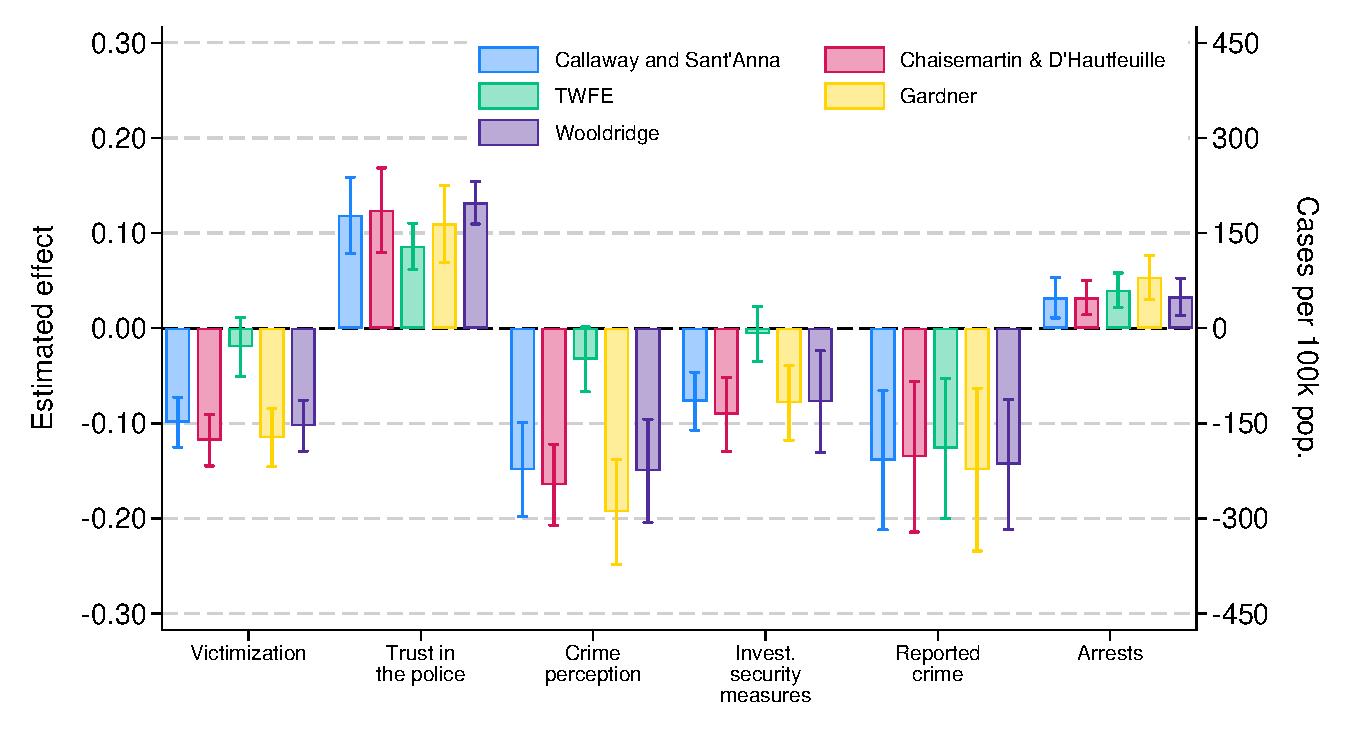
\includegraphics[width=\textwidth]{../manuscript/Graphs/Comparison_estimators_combined.pdf}
    \\[8pt]
    \begin{minipage}{0.99\textwidth}
    \footnotesize Notes: The figure reports the effects of \emph{Plan Cuadrante} on different measures of police effectiveness using various difference-in-differences estimators, including the methods developed in \citet{Callaway}, \citet{Chaisemartin}, \citet{Gardner}, \citet{wooldridge2023simple}, and the canonical two-way fixed effects (TWFE). Bars are the estimated post-treatment effects and the whiskers the 95\% confidence intervals; standard errors are clustered at the municipality level. Victimization is the probability of household victimization in the last 12 months; reported crime is the number of crimes reported to the police in the municipality per 100,000 inhabitants; crime perception is the probability of perceiving an increase in crime; investment in security measures is the probability of adopting security measures in the last twelve months; trust in the police is the probability of reporting high trust in the police; and arrests is the number of arrests per 100,000 inhabitants. Reported crime and arrests (administrative data) are read on the right axis; all other outcomes, from the ENUSC survey, are read on the left axis.
    \end{minipage}
\end{figure}


Figures \ref{fig:alterestim_delitos} through \ref{fig:alterestim_crime} report the corresponding event-study estimates for victimization, crime perception, investment in security measures, and reported crime under each alternative estimator. Pre-treatment coefficients are consistently small and statistically indistinguishable from zero across all estimators and outcomes, confirming that the parallel trends assumption holds regardless of the estimation method. Post-treatment effects remain negative and statistically significant across these outcomes, closely mirroring the results from the main specification in Figure \ref{fig:figure02}.

% =============================================================================
% Alternative-estimator robustness figures
% Each figure shows the event study from three estimators:
%   (a) Chaisemartin & D'Hautfeuille
%   (b) Gardner
%   (c) Wooldridge
% Callaway & Sant'Anna is excluded — it appears as the headline figure.
%
% First block (3 figures): ENUSC survey outcomes
% Second block (1 figure): SPD administrative crime outcomes
% =============================================================================


% ----- Victimization (delitos) -----------------------------------------------
\begin{figure}[h!]
    \centering
    \caption[Effects of \emph{Plan Cuadrante} on Victimization Using Alternative Estimators]{Effects of \emph{Plan Cuadrante} on Victimization Using Alternative Estimators}
    \label{fig:alterestim_delitos}
    \begin{subfigure}{0.47\textwidth}
        \centering
        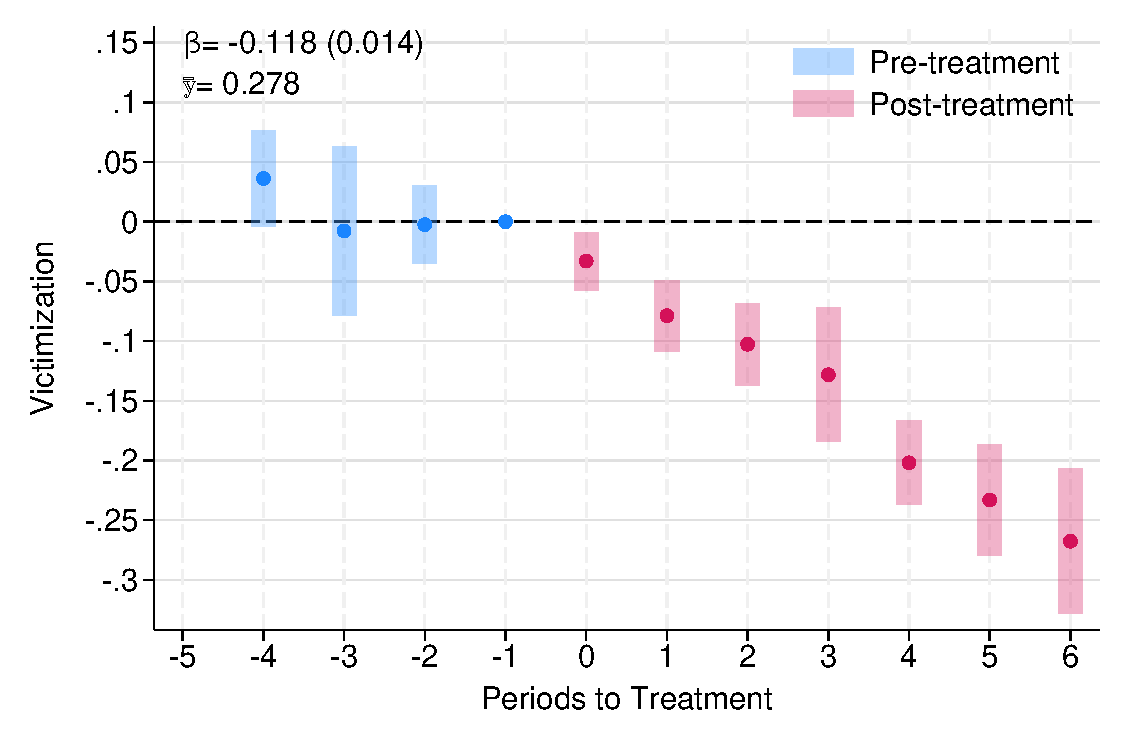
\includegraphics[width=\textwidth]{../manuscript/Graphs/CHDH_event_study_delitos.pdf}
        \caption{Chaisemartin \& D'Hautfeuille}
    \end{subfigure}%
    \begin{subfigure}{0.47\textwidth}
        \centering
        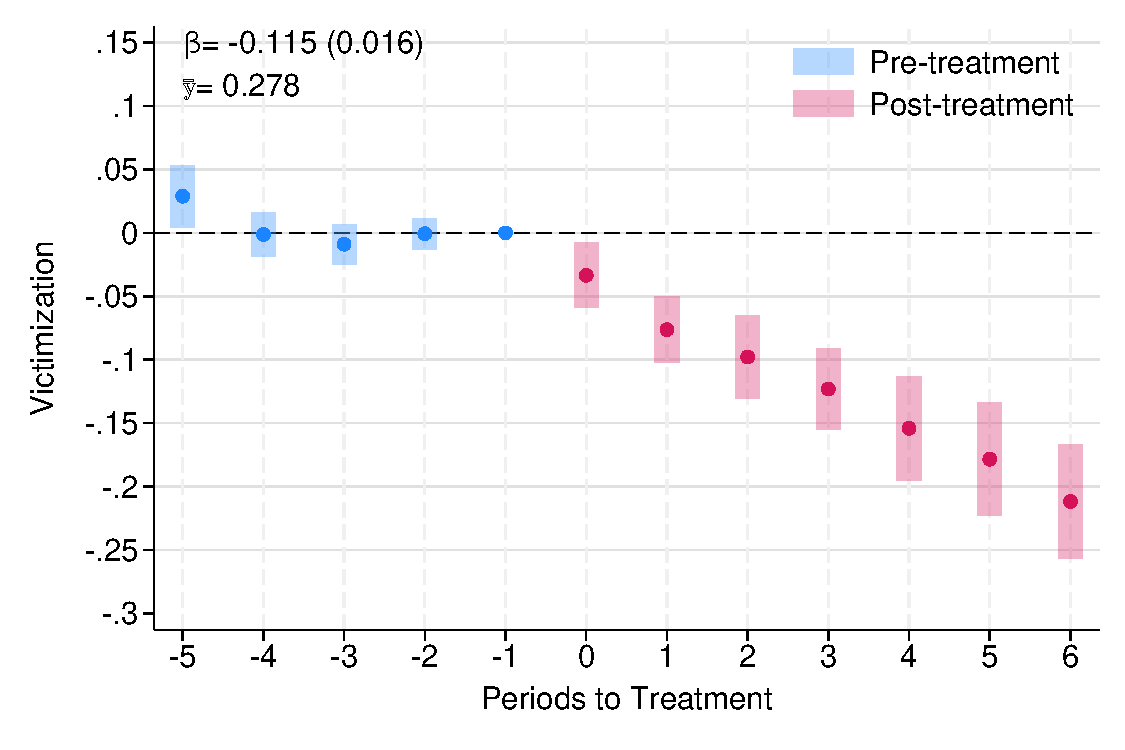
\includegraphics[width=\textwidth]{../manuscript/Graphs/DID2S_event_study_delitos.pdf}
        \caption{Gardner}
    \end{subfigure}
    \\[6pt]
    \begin{subfigure}{0.47\textwidth}
        \centering
        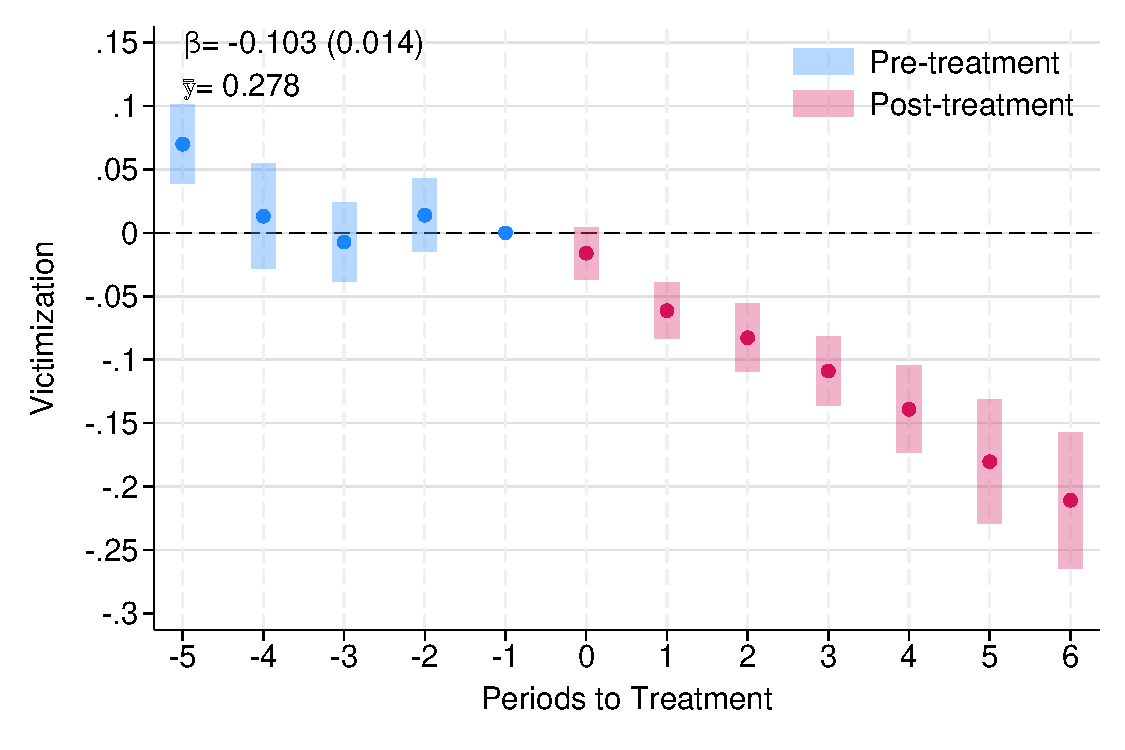
\includegraphics[width=\textwidth]{../manuscript/Graphs/JWDID_event_study_delitos.pdf}
        \caption{Wooldridge}
    \end{subfigure}
    \\[12pt]
    \begin{minipage}{0.99\textwidth}
    \footnotesize Notes: The figure reports event-study estimates of the effect of \emph{Plan Cuadrante} on the probability of household victimization in the last 12 months using the ENUSC survey, estimated with three alternative difference-in-differences estimators robust to staggered adoption: \citet{Chaisemartin} in panel (a), \citet{Gardner} in panel (b), and \citet{wooldridge2023simple} in panel (c). Each panel plots the estimated coefficient at each event time relative to treatment along with 95\% confidence intervals. Standard errors are clustered at the municipality level. The headline coefficient $\beta$ corresponds to the average post-treatment effect, and $\bar{y}$ denotes the never-treated mean of the outcome over the sample period.
    \end{minipage}
\end{figure}


% ----- Crime perception (inseguridad_barrio1) --------------------------------
\begin{figure}[h!]
    \centering
    \caption[Effects of \emph{Plan Cuadrante} on Crime Perception Using Alternative Estimators]{Effects of \emph{Plan Cuadrante} on Crime Perception Using Alternative Estimators}
    \label{fig:alterestim_inseguridad}
    \begin{subfigure}{0.47\textwidth}
        \centering
        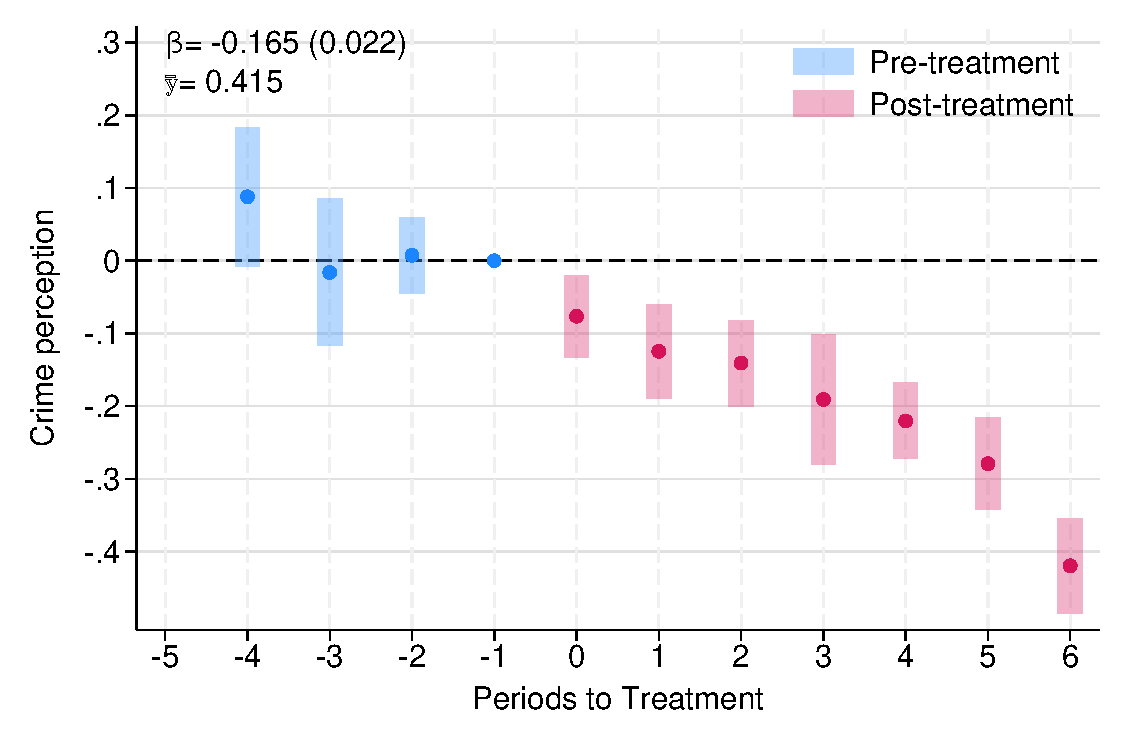
\includegraphics[width=\textwidth]{../manuscript/Graphs/CHDH_event_study_inseguridad_barrio1.pdf}
        \caption{Chaisemartin \& D'Hautfeuille}
    \end{subfigure}%
    \begin{subfigure}{0.47\textwidth}
        \centering
        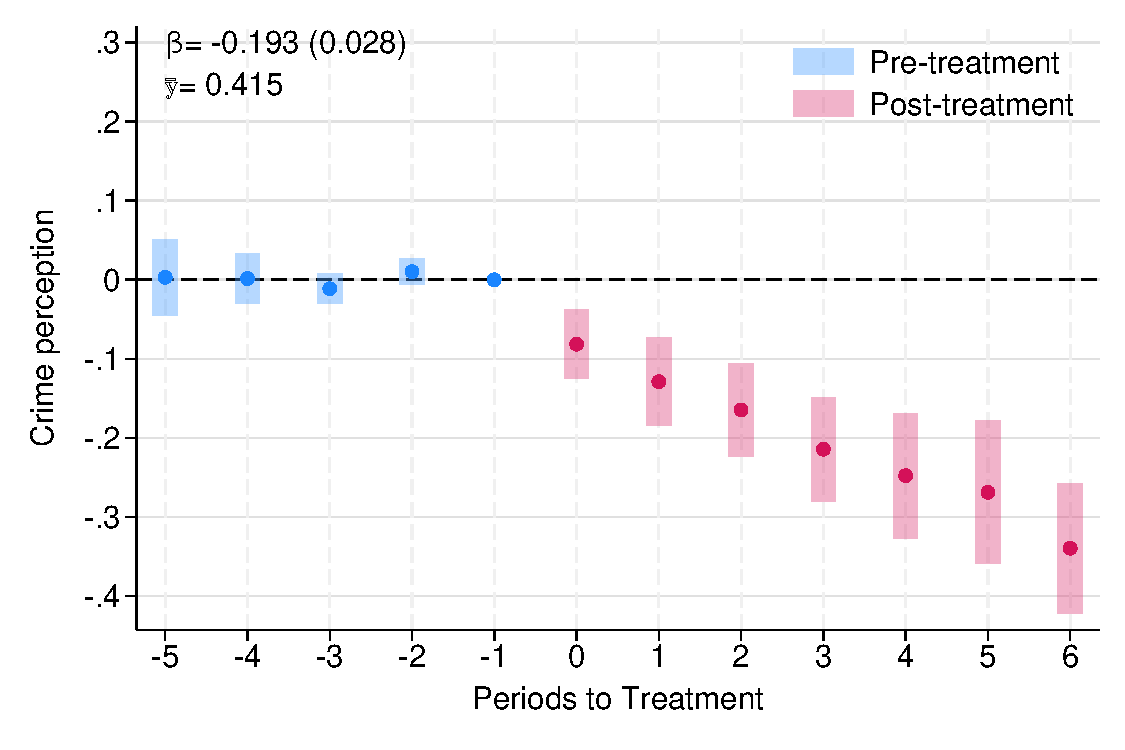
\includegraphics[width=\textwidth]{../manuscript/Graphs/DID2S_event_study_inseguridad_barrio1.pdf}
        \caption{Gardner}
    \end{subfigure}
    \\[6pt]
    \begin{subfigure}{0.47\textwidth}
        \centering
        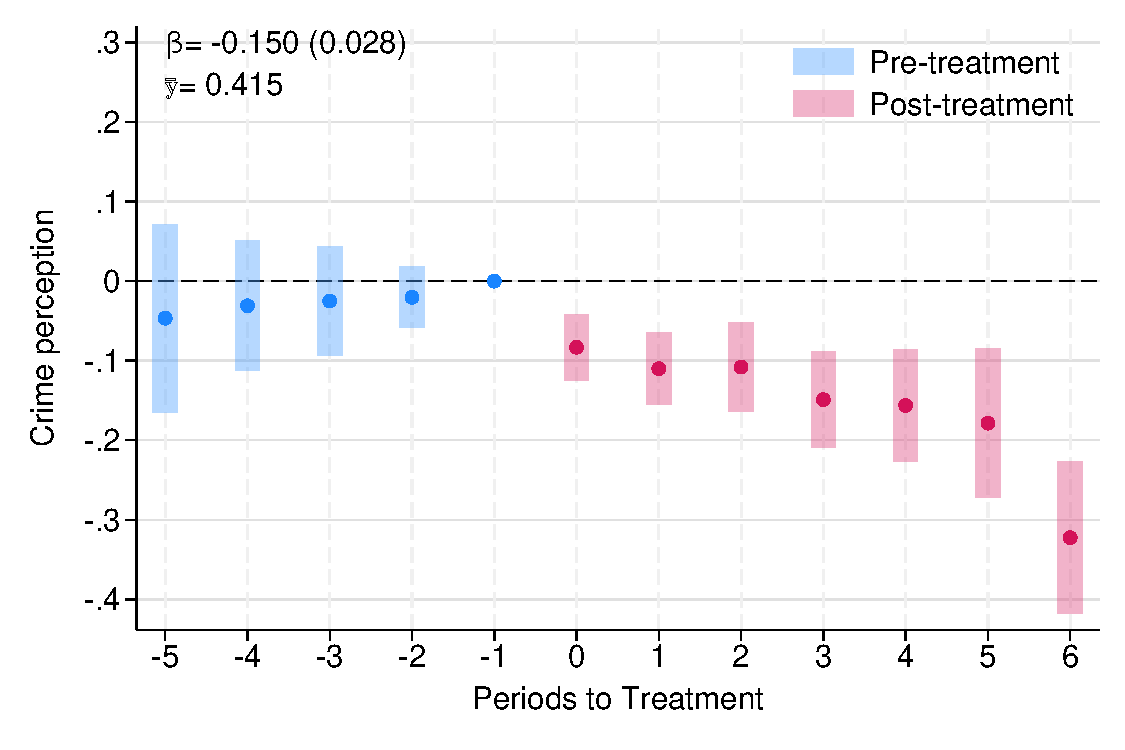
\includegraphics[width=\textwidth]{../manuscript/Graphs/JWDID_event_study_inseguridad_barrio1.pdf}
        \caption{Wooldridge}
    \end{subfigure}
    \\[12pt]
    \begin{minipage}{0.99\textwidth}
    \footnotesize Notes: The figure reports event-study estimates of the effect of \emph{Plan Cuadrante} on the probability of perceiving an increase in crime using the ENUSC survey, estimated with three alternative difference-in-differences estimators robust to staggered adoption: \citet{Chaisemartin} in panel (a), \citet{Gardner} in panel (b), and \citet{wooldridge2023simple} in panel (c). Each panel plots the estimated coefficient at each event time relative to treatment along with 95\% confidence intervals. Standard errors are clustered at the municipality level. The headline coefficient $\beta$ corresponds to the average post-treatment effect, and $\bar{y}$ denotes the never-treated mean of the outcome over the sample period.
    \end{minipage}
\end{figure}


% ----- Private investment in security (medidas_general_12) -------------------
\begin{figure}[h!]
    \centering
    \caption[Effects of \emph{Plan Cuadrante} on Investment in Security Measures Using Alternative Estimators]{Effects of \emph{Plan Cuadrante} on Investment in Security Measures Using Alternative Estimators}
    \label{fig:alterestim_medidas}
    \begin{subfigure}{0.47\textwidth}
        \centering
        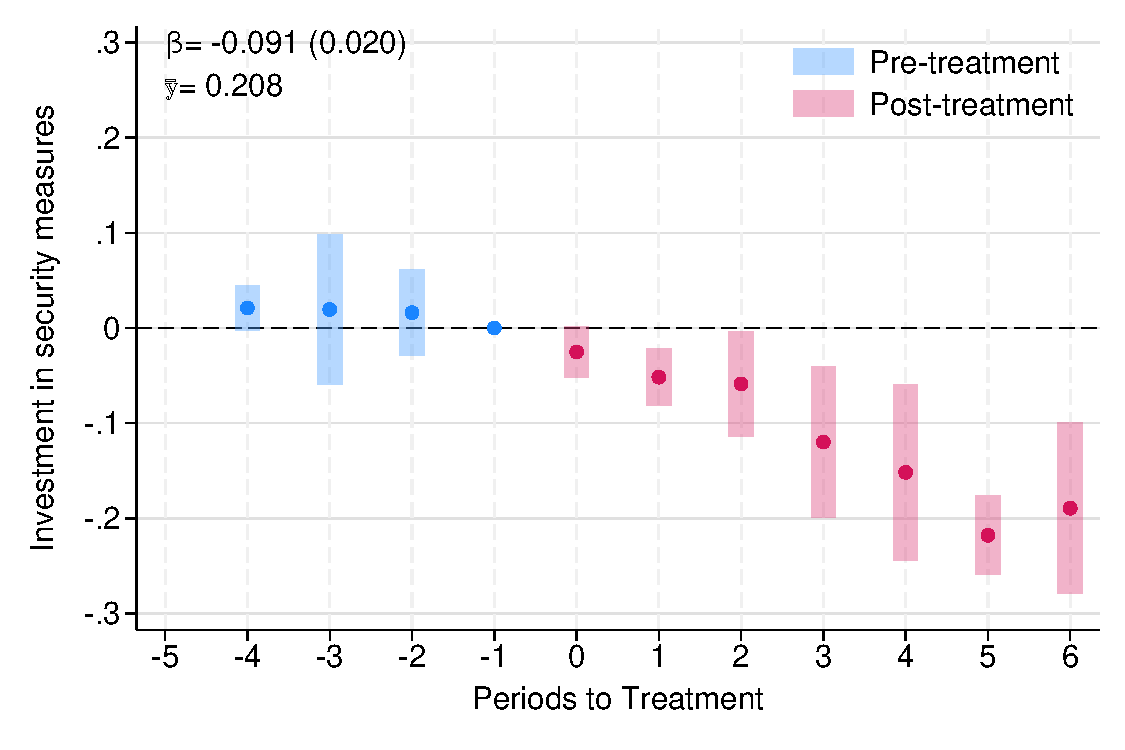
\includegraphics[width=\textwidth]{../manuscript/Graphs/CHDH_event_study_medidas_general_12.pdf}
        \caption{Chaisemartin \& D'Hautfeuille}
    \end{subfigure}%
    \begin{subfigure}{0.47\textwidth}
        \centering
        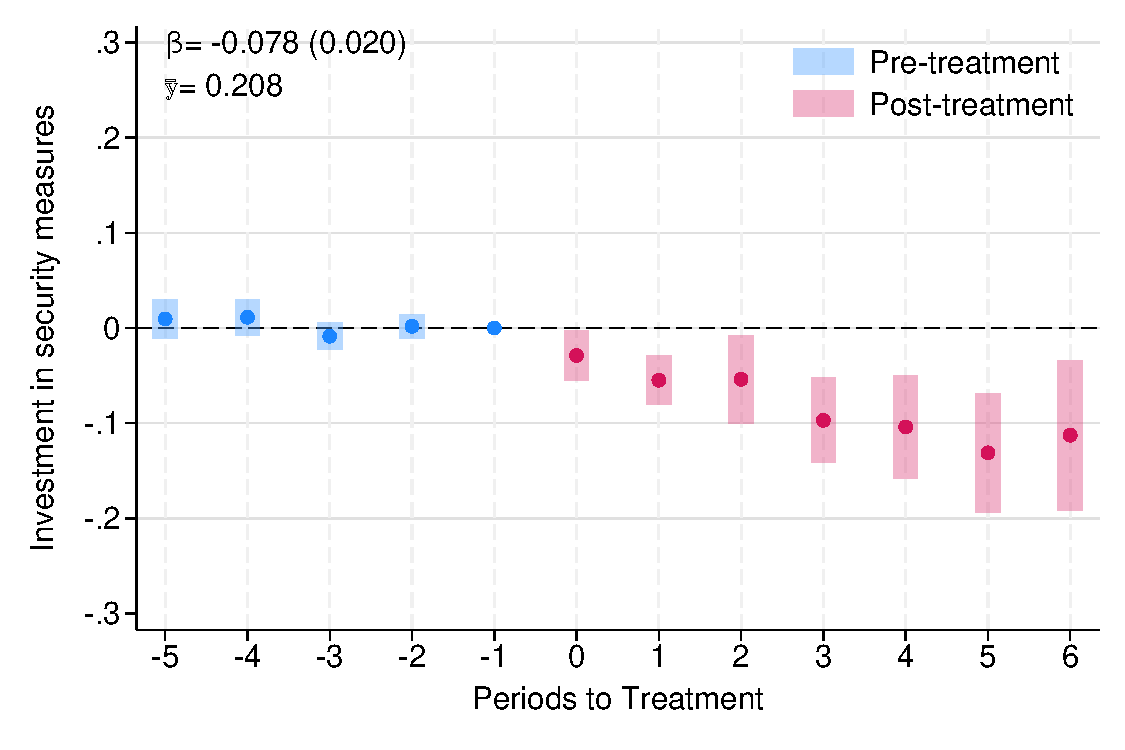
\includegraphics[width=\textwidth]{../manuscript/Graphs/DID2S_event_study_medidas_general_12.pdf}
        \caption{Gardner}
    \end{subfigure}
    \\[6pt]
    \begin{subfigure}{0.47\textwidth}
        \centering
        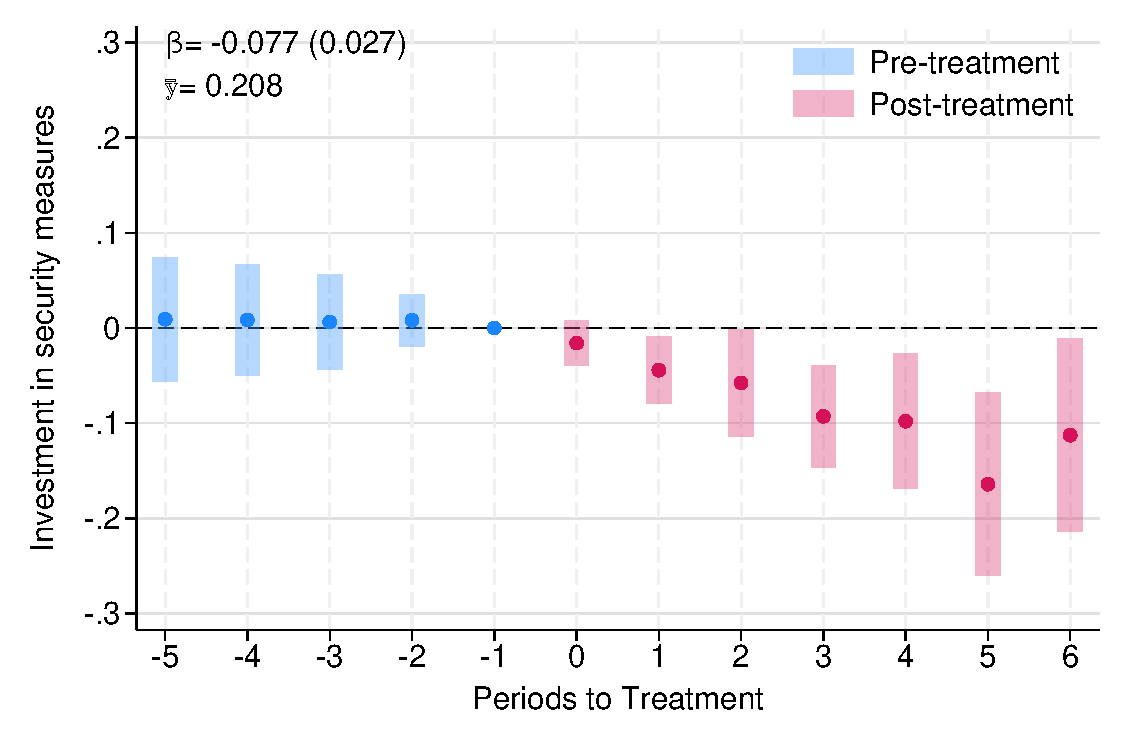
\includegraphics[width=\textwidth]{../manuscript/Graphs/JWDID_event_study_medidas_general_12.pdf}
        \caption{Wooldridge}
    \end{subfigure}
    \\[12pt]
    \begin{minipage}{0.99\textwidth}
    \footnotesize Notes: The figure reports event-study estimates of the effect of \emph{Plan Cuadrante} on the probability of adopting security measures in the last twelve months using the ENUSC survey, estimated with three alternative difference-in-differences estimators robust to staggered adoption: \citet{Chaisemartin} in panel (a), \citet{Gardner} in panel (b), and \citet{wooldridge2023simple} in panel (c). Each panel plots the estimated coefficient at each event time relative to treatment along with 95\% confidence intervals. Standard errors are clustered at the municipality level. The headline coefficient $\beta$ corresponds to the average post-treatment effect, and $\bar{y}$ denotes the never-treated mean of the outcome over the sample period.
    \end{minipage}
\end{figure}


% =============================================================================
% Administrative data (SPD municipality-level)
% =============================================================================


% ----- Reported crime --------------------------------------------------------
\begin{figure}[h!]
    \centering
    \caption[Effects of \emph{Plan Cuadrante} on Reported Crime Using Alternative Estimators]{Effects of \emph{Plan Cuadrante} on Reported Crime Using Alternative Estimators}
    \label{fig:alterestim_crime}
    \begin{subfigure}{0.47\textwidth}
        \centering
        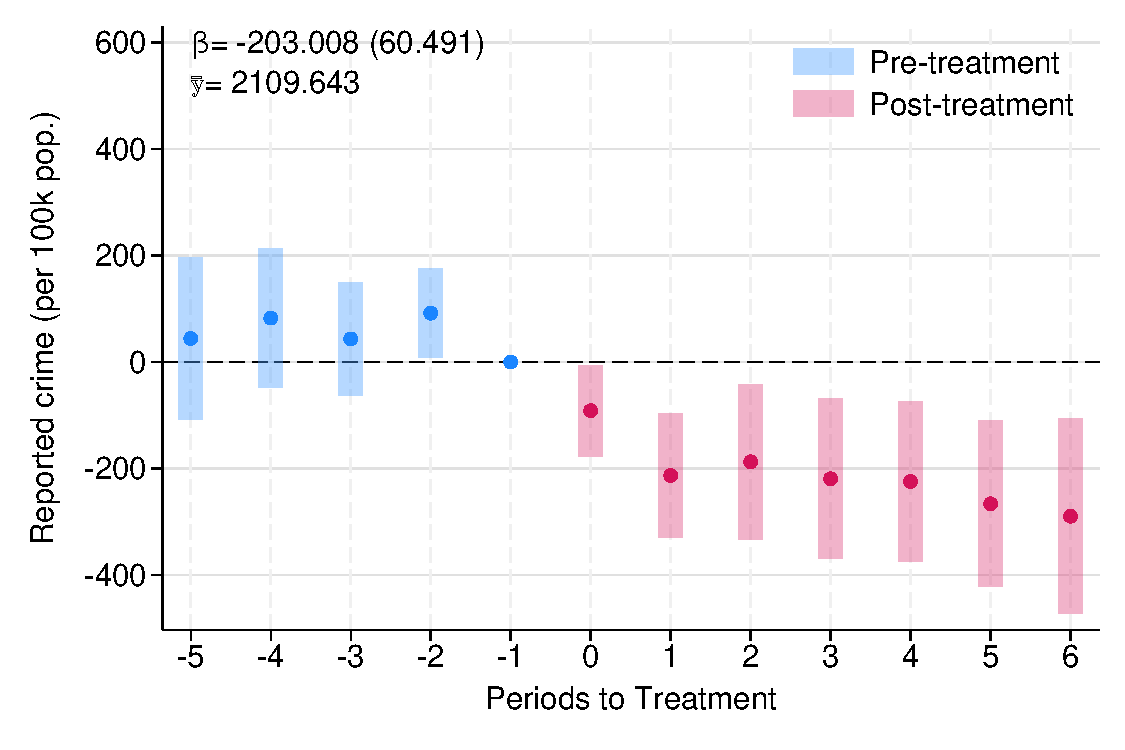
\includegraphics[width=\textwidth]{../manuscript/Graphs/CHDH_event_study_crime.pdf}
        \caption{Chaisemartin \& D'Hautfeuille}
    \end{subfigure}%
    \begin{subfigure}{0.47\textwidth}
        \centering
        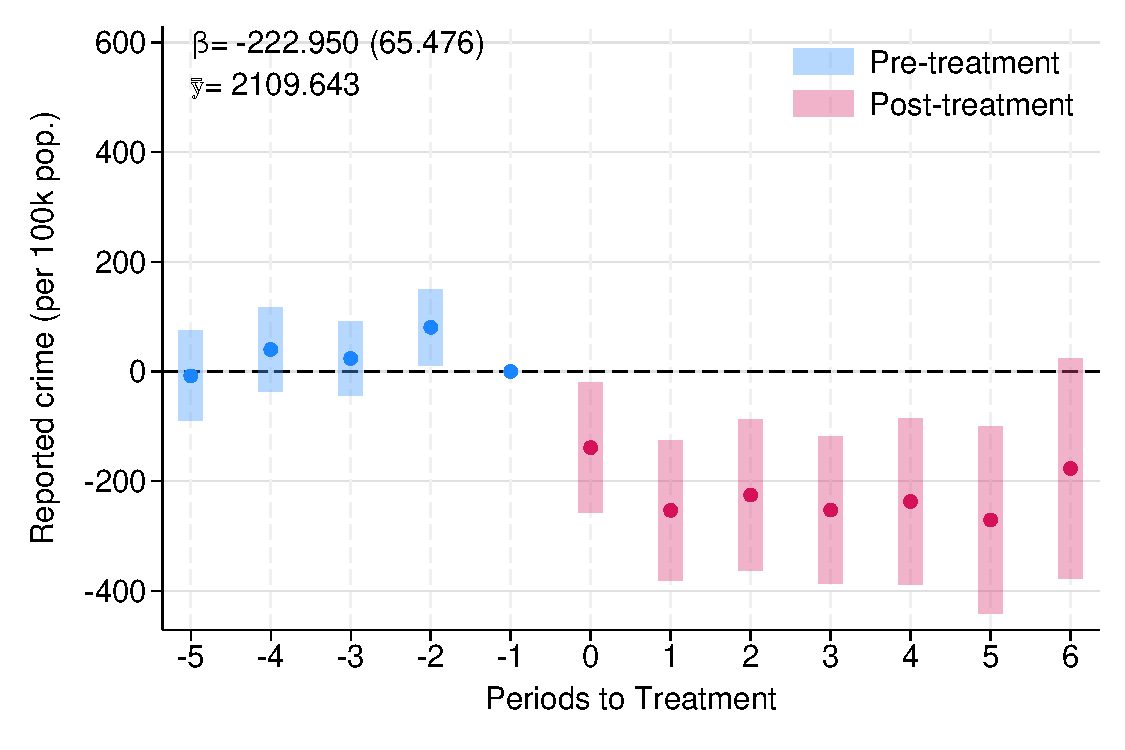
\includegraphics[width=\textwidth]{../manuscript/Graphs/DID2S_event_study_crime.pdf}
        \caption{Gardner}
    \end{subfigure}
    \\[6pt]
    \begin{subfigure}{0.47\textwidth}
        \centering
        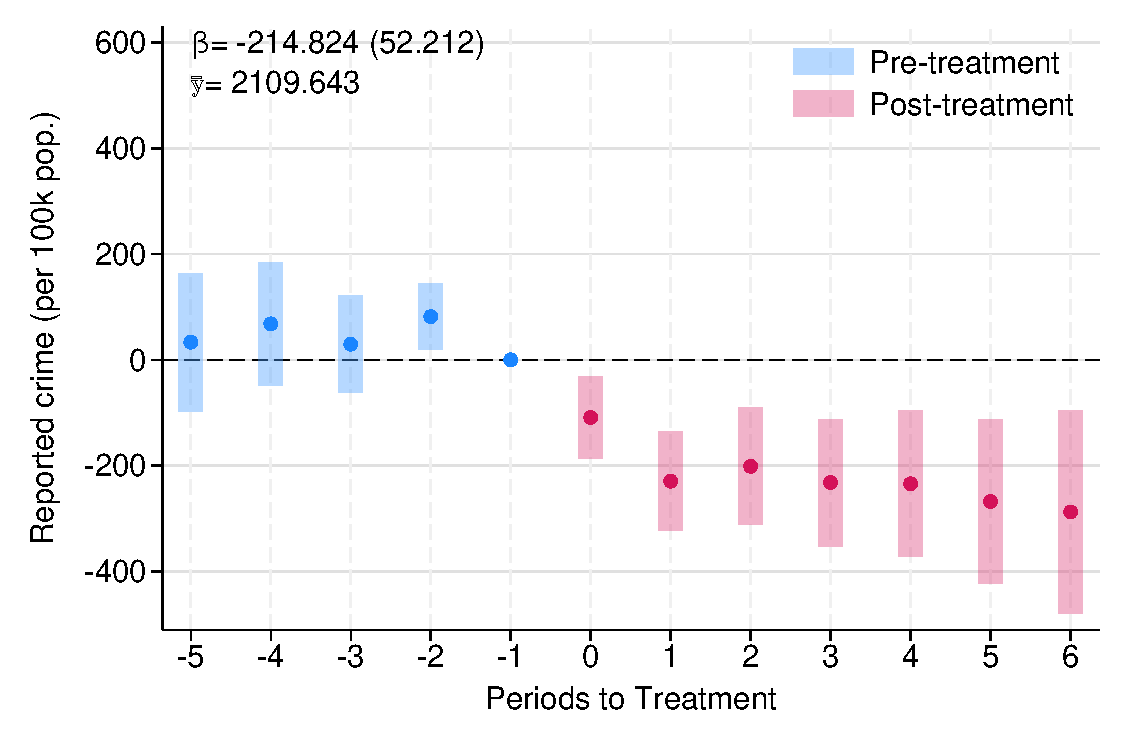
\includegraphics[width=\textwidth]{../manuscript/Graphs/JWDID_event_study_crime.pdf}
        \caption{Wooldridge}
    \end{subfigure}
    \\[12pt]
    \begin{minipage}{0.99\textwidth}
    \footnotesize Notes: The figure reports event-study estimates of the effect of \emph{Plan Cuadrante} on the number of crimes reported to the police in the municipality per 100,000 inhabitants using administrative data, estimated with three alternative difference-in-differences estimators robust to staggered adoption: \citet{Chaisemartin} in panel (a), \citet{Gardner} in panel (b), and \citet{wooldridge2023simple} in panel (c). Each panel plots the estimated coefficient at each event time relative to treatment along with 95\% confidence intervals. Standard errors are clustered at the municipality level. The headline coefficient $\beta$ is the equal-weighted average of the post-treatment effects from $t=0$ to $t=6$, and $\bar{y}$ denotes the never-treated mean of the outcome over the sample period.
    \end{minipage}
\end{figure}

\clearpage

\subsection{Effects of \emph{Plan Cuadrante} using a Balanced Panel}

Figure \ref{fig:figureA6_bp} shows the effects of \emph{Plan Cuadrante} on the main outcomes, but estimated using a balanced panel of municipalities. For the ENUSC-based outcomes, this panel includes only municipalities that implemented the \emph{Plan Cuadrante} between 2006 and 2009, which allows the construction of a balanced panel from t-2 to t+3 (31 municipalities). For the administrative outcomes, the balanced panel comprises those municipalities observed over that same t-2 to t+3 window around their own adoption (94 for reported crime and 78 for arrests). The resulting estimates are very similar to those presented in the main document.

\begin{figure}[h!]
    \centering
    \caption{Effects of \emph{Plan Cuadrante} Using a Balanced Panel of Municipalities}
    \label{fig:figureA6_bp}
    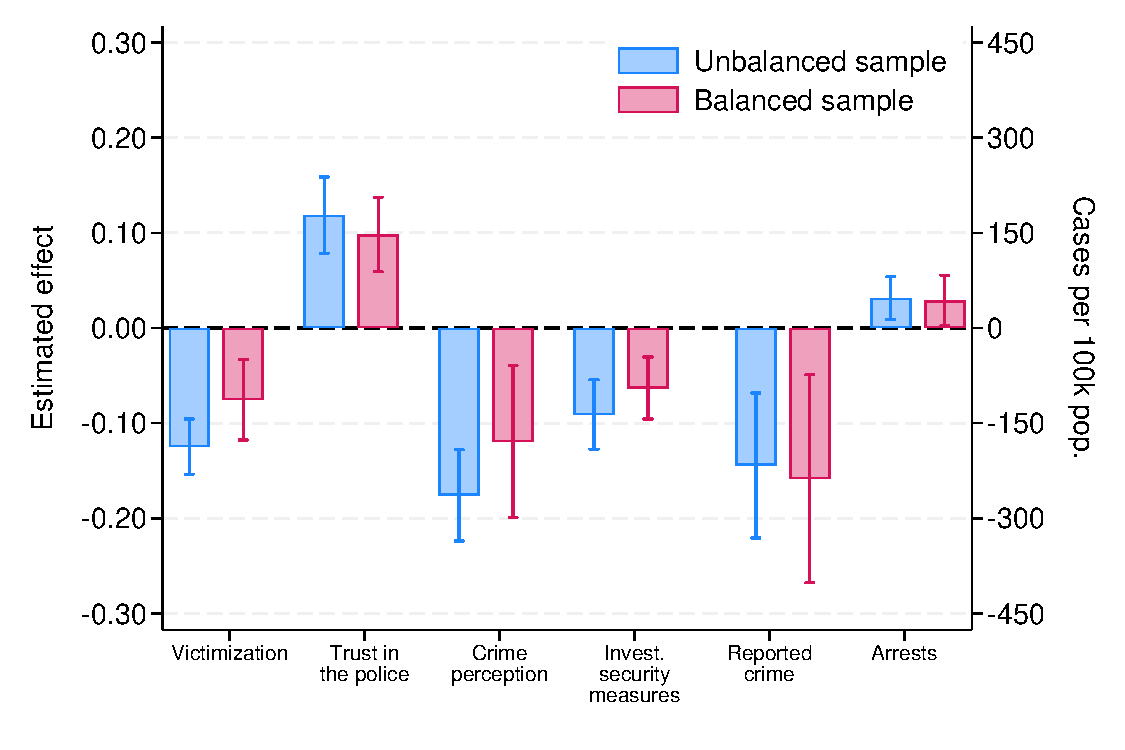
\includegraphics[width=0.8\textwidth]{../manuscript/Graphs/results_crime_balanced_combined.pdf}
    \\[10pt]
    \begin{minipage}{0.99\textwidth}
    \footnotesize Notes: The figure reports the effects of \emph{Plan Cuadrante} on different measures of police effectiveness using the main analytical sample (unbalanced, blue bars) and a balanced panel of municipalities observed over the full event-study window from $t-2$ to $t+3$ (red bars). For the ENUSC sample the balanced panel consists of the 31 municipalities that implemented \emph{Plan Cuadrante} between 2006 and 2009; for the administrative municipality-level sample it consists of 94 municipalities for reported crime and 78 municipalities for arrests. The bars represent the average post-treatment effect estimated with the difference-in-differences estimator developed in \citet{Callaway}, and the whiskers the 95\% confidence intervals; standard errors are clustered at the municipality level. Victimization is the probability of household victimization in the last 12 months; reported crime is the number of crimes reported to the police in the municipality per 100,000 inhabitants; arrests is the number of arrests per 100,000 inhabitants; trust in the police is the probability of reporting high trust in the police; crime perception is the probability of perceiving an increase in crime; and investment in security measures is the probability of adopting security measures in the last twelve months. Reported crime and arrests (administrative data) are read on the right axis; all other outcomes, from the ENUSC survey, are read on the left axis.
    \end{minipage}
\end{figure}

\clearpage

\subsection{Effects of \emph{Plan Cuadrante} Using the Full Set of Post-treatment and Pre-treatment Periods}
\label{sec:admin_uncapped}

For symmetry with the ENUSC-based analysis, the event studies for reported crime and arrests reported in the main text are restricted to 5 pre-treatment and 7 post-treatment periods. Because the administrative data are available for the full set of Chilean municipalities and therefore include a much larger number of never-treated municipalities than the ENUSC sample, we can estimate these effects over a longer window without exhausting the pool of valid comparison units. Figure \ref{fig:admin_uncapped} reports the effects of \emph{Plan Cuadrante} on reported crime and arrests using the full set of post-treatment and pre-treatment periods rather than capping the event study to the 5 pre-treatment and 7 post-treatment periods used in the main specification. The results are very similar to those presented in Section \ref{main_results}.

\begin{figure}[h!]
    \centering
    \caption{Effects of \emph{Plan Cuadrante} on Reported Crime and Arrests Using the Full Set of Post-treatment and Pre-treatment Periods}
    \label{fig:admin_uncapped}
    \begin{subfigure}{0.495\textwidth}
        \centering
        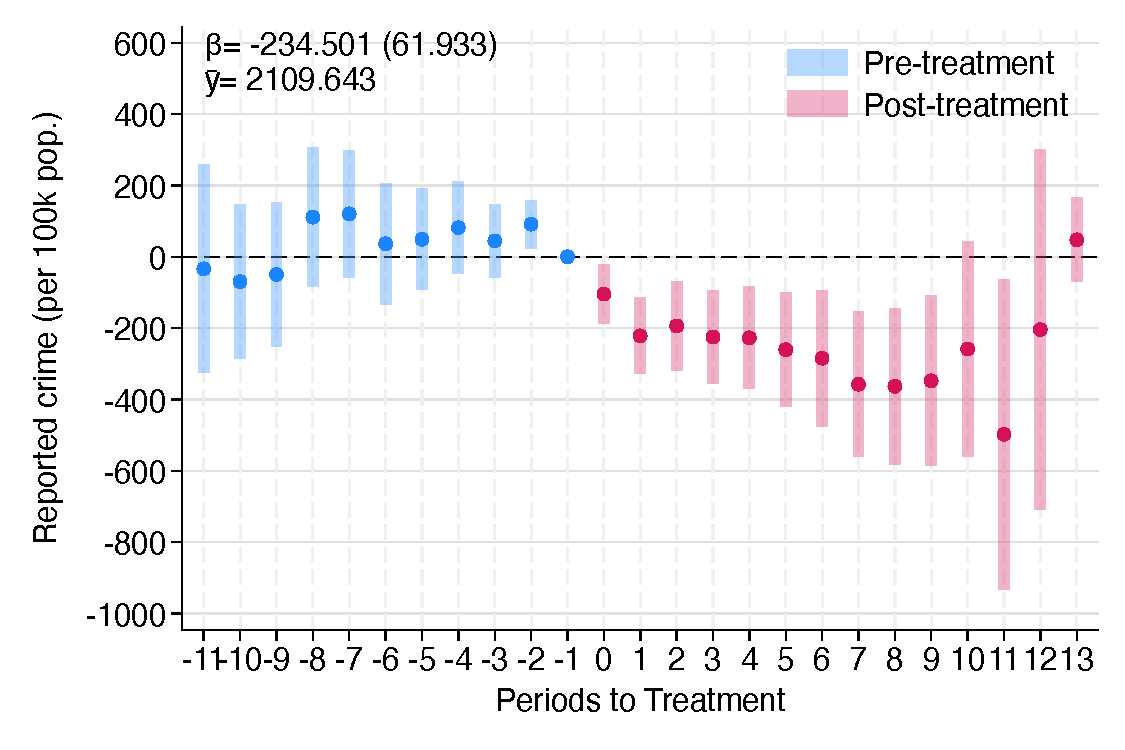
\includegraphics[width=0.98\textwidth]{../manuscript/Graphs/totalreportedcrime_allcomunas_uncapped.pdf}
        \caption{Reported crime per 100k inhabitants}
    \end{subfigure}%
    ~
    \begin{subfigure}{0.495\textwidth}
    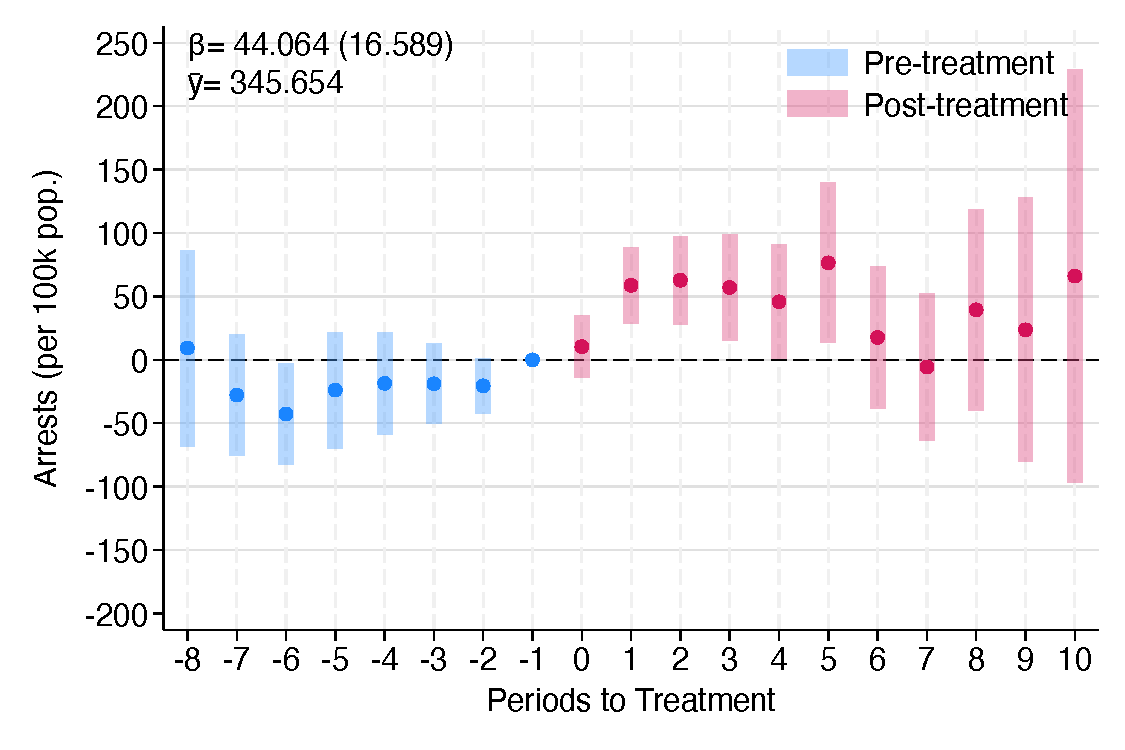
\includegraphics[width=0.98\textwidth]{../manuscript/Graphs/totalarrestscrime_allcomunas_uncapped.pdf}
        \caption{Arrests per 100k inhabitants}
    \end{subfigure}
    \begin{minipage}{\textwidth}
    \footnotesize
   Notes: This figure shows the dynamic effects of \emph{Plan Cuadrante} on the number of crimes reported to the police in the municipality per 100,000 inhabitants (panel a) and on the number of arrests in the municipality per 100,000 inhabitants (panel b), using administrative data. The estimation is conducted using the procedure developed in \citet{Callaway} for difference-in-differences with staggered treatment adoption. The dots in the figure represent the estimated coefficients and the bars behind them 95\% confidence intervals. Standard errors are clustered at the municipality level using the wild bootstrapping procedure. The pooled effect and the mean outcome before the introduction of the treatment are also presented in each panel. Unlike Figure \ref{fig:figure02} in the main text, we do not cap the event study to the same 5 pre-treatment and 6 post-treatment periods used for symmetry with the ENUSC-based analysis. Instead, we exploit the full set of post-treatment and pre-treatment periods. Panel (a) includes 4,371 observations and panel (b) 3,372 observations.
    \end{minipage}
\end{figure}

\clearpage

\subsection{Multiple Hypothesis Testing}
\label{sec:bonferroni}

Testing multiple outcomes simultaneously raises concerns about false discoveries. In our analyses, all six outcomes in our main analyses are statistically significant at the 1\% significance level. Under the null hypothesis of no effects, one would expect at most 1\% of tested coefficients to be false positives by chance at the same level. The observed pattern of results is therefore difficult to reconcile with false discoveries driven by multiple testing. Nonetheless, to address this concern formally, we apply a multiple hypothesis testing correction to the p-values. While procedures such as \citet{romano2005} would be a natural choice, their implementation is not computationally straightforward with the \citet{Callaway} estimator. We therefore apply the Bonferroni correction, which can be applied directly to any set of estimated p-values regardless of the underlying estimator. The adjusted p-values, reported in Table \ref{tab:bonferroni}, confirm that the main results remain statistically significant at conventional confidence levels after correction for every outcome considered.

\begin{table}[H]
\centering
\caption{Multiple Hypothesis Testing: Bonferroni Correction}
\label{tab:bonferroni}
\begin{tabular}{lcccc}
\toprule
Outcome & \multicolumn{2}{c}{} & \multicolumn{2}{c}{Bonferroni} \\
 & \multicolumn{2}{c}{Original} & \multicolumn{2}{c}{adjusted} \\
\cmidrule(lr){2-3} \cmidrule(lr){4-5}
 & p-value & & p-value & \\
\midrule
Victimization & 0.00000 & *** & 0.00000 & *** \\
Reported crime (per 100k pop.) & 0.00021 & *** & 0.00126 & *** \\
Crime perception & 0.00000 & *** & 0.00000 & *** \\
Investment in security measures & 0.00000 & *** & 0.00000 & *** \\
Trust in the police & 0.00000 & *** & 0.00000 & *** \\
Arrests (per 100k pop.) & 0.00316 & *** & 0.01896 & ** \\
\midrule
\multicolumn{5}{l}{\footnotesize Notes: Bonferroni correction multiplies each p-value by the number of} \\
\multicolumn{5}{l}{\footnotesize outcomes tested ($n=6$). Significance levels: *** $p<0.01$, ** $p<0.05$, * $p<0.1$.}
\end{tabular}
\end{table}
\clearpage

\subsection{Placebo Test Using Non-neighborhood Crime}

To assess whether the observed decline in crime is driven by broader temporal trends rather than increased police presence, we conduct a placebo test using a type of crime unlikely to be affected by beat policing—namely, non-neighborhood crime such as sexual abuse. These crimes typically occur outside the scope of routine neighborhood patrols and are therefore not expected to respond directly to changes in local police deployment. We use annual municipal-level data on reported sexual abuse and related arrests from 2005 to 2016, obtained from the Undersecretary for Crime Prevention.

Figure~\ref{fig:figureA9} shows that the implementation of \emph{Plan Cuadrante} is, as expected, not significantly associated with changes in sexual abuse crime.

\begin{figure}[h!]
    \centering
    \caption{The Effects of \emph{Plan Cuadrante} on Sexual Abuse}
    \label{fig:figureA9}
    \begin{subfigure}{0.495\textwidth}
        \centering
        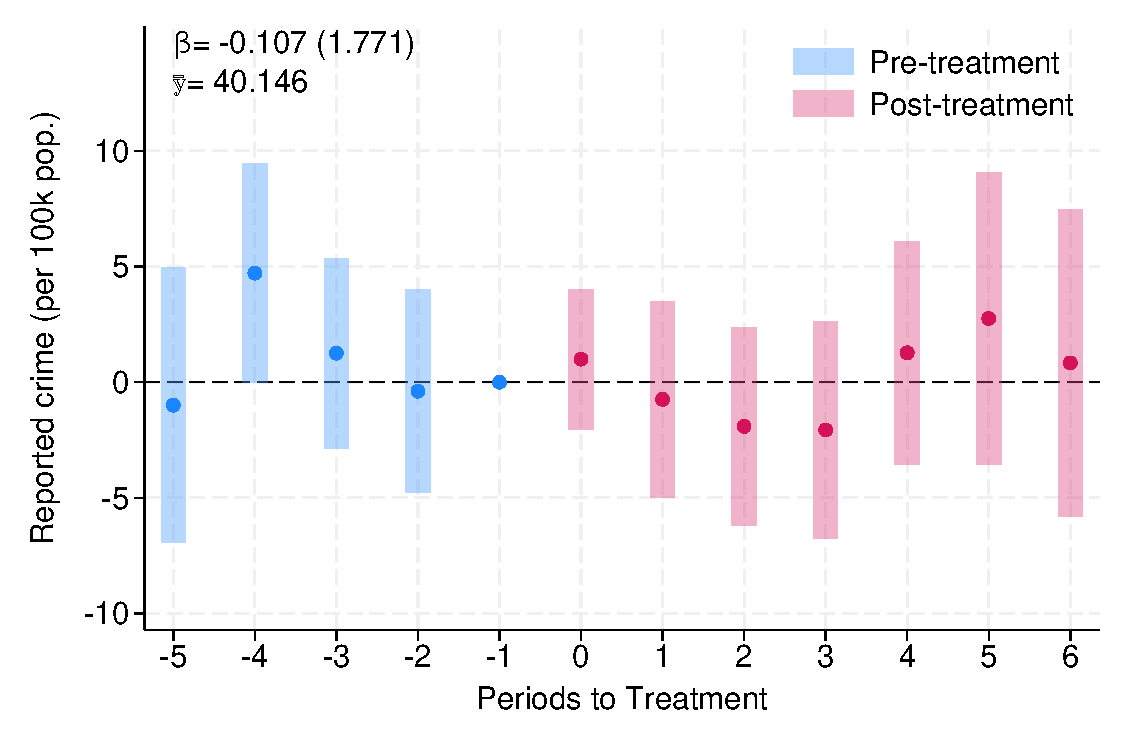
\includegraphics[width=\textwidth]{../manuscript/Graphs/results_sexualabuse.pdf}
                \caption{Reported crime per 100k inhabitants}
    \end{subfigure}%
    ~
    \begin{subfigure}{0.495\textwidth}
        \centering
        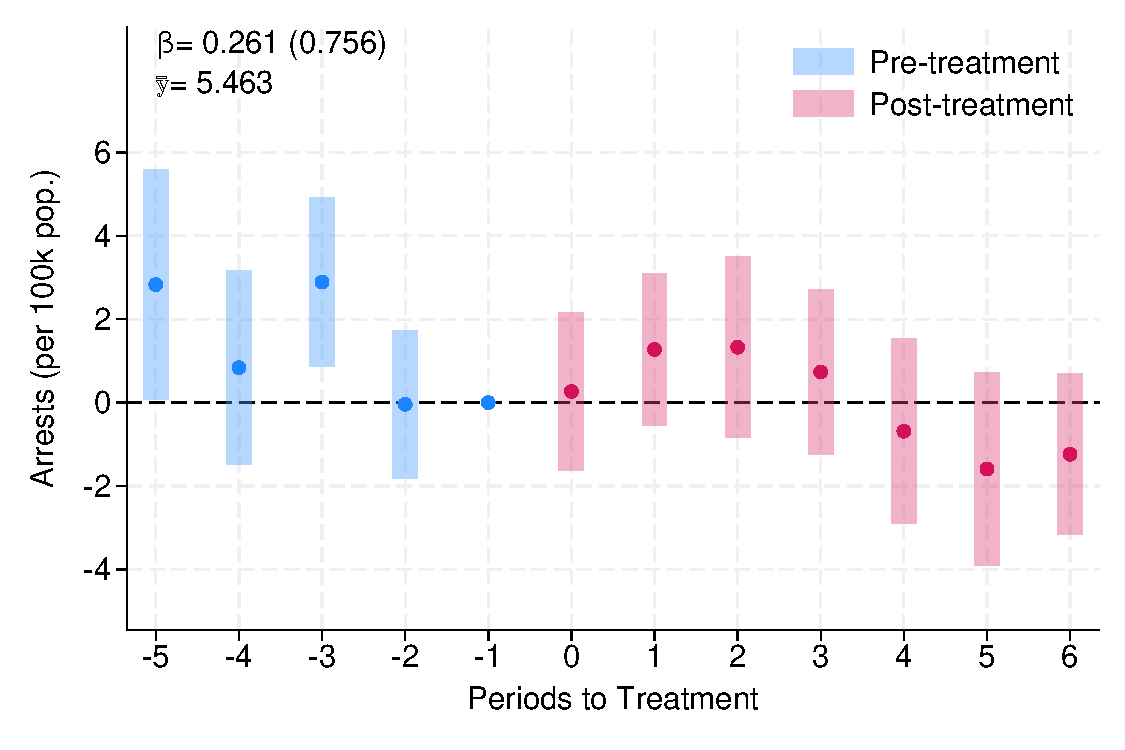
\includegraphics[width=\textwidth]{../manuscript/Graphs/results_sexualabuse2.pdf}
                \caption{Arrests per 100k inhabitants}
    \end{subfigure}
    \\[12pt]
    \begin{minipage}{0.99\textwidth}
    \footnotesize Notes: This figure shows the dynamic effects of the \emph{Plan Cuadrante} on sexual abuse per 100,000 inhabitants. The estimation is conducted using the procedure developed in \citet{Callaway} for difference-in-differences with staggered treatment adoption. The graphs display the estimated coefficients and 95\% confidence intervals. Standard errors are clustered at the municipality level using the wild bootstrapping procedure.
    \end{minipage}
\end{figure}
\clearpage

\subsection{The Effects of \emph{Plan Cuadrante} on Other Measures of Crime Perception}

The results reported in panel (c) of Figure \ref{fig:figure02} showed that \emph{Plan Cuadrante} decreased households' perception of crime in the neighborhood. However, the ENUSC survey not only asks about individuals' crime perception in the neighborhood, but also in the municipality and in the country. Figure \ref{fig:figureA3} reports the results of \emph{Plan Cuadrante} on the perception of crime in the municipality and in the country. While the effect is consistently negative and statistically significant also for these measures of crime perception, the effect is much smaller for insecurity in the country, indicating that the effects of the program on crime perception are larger at the local level.

\begin{figure}[h!]
    \centering
    \caption{Effects of \emph{Plan Cuadrante} on Crime Perception in the Municipality and in the Country}
    \label{fig:figureA3}
    \begin{subfigure}{0.495\textwidth}
        \centering
        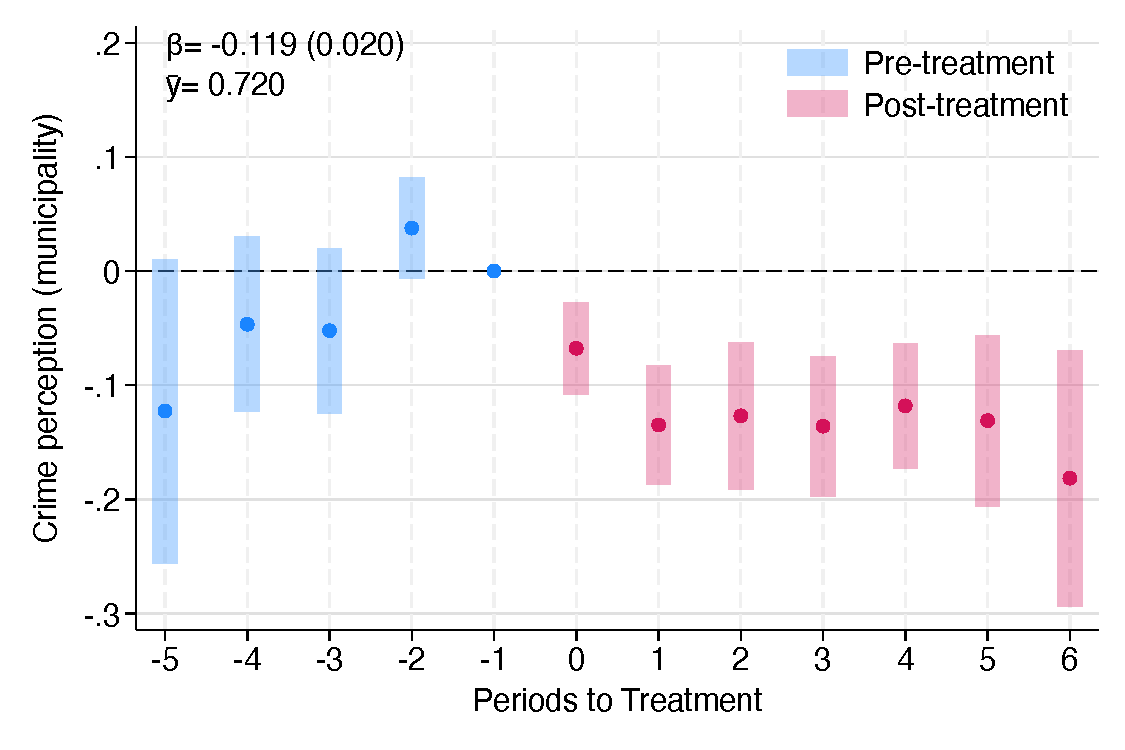
\includegraphics[width=\textwidth]{../manuscript/Graphs/results_perception_municipality.pdf}
        \caption{In the municipality}
    \end{subfigure}%
    ~ 
    \begin{subfigure}{0.495\textwidth}
    \centering
    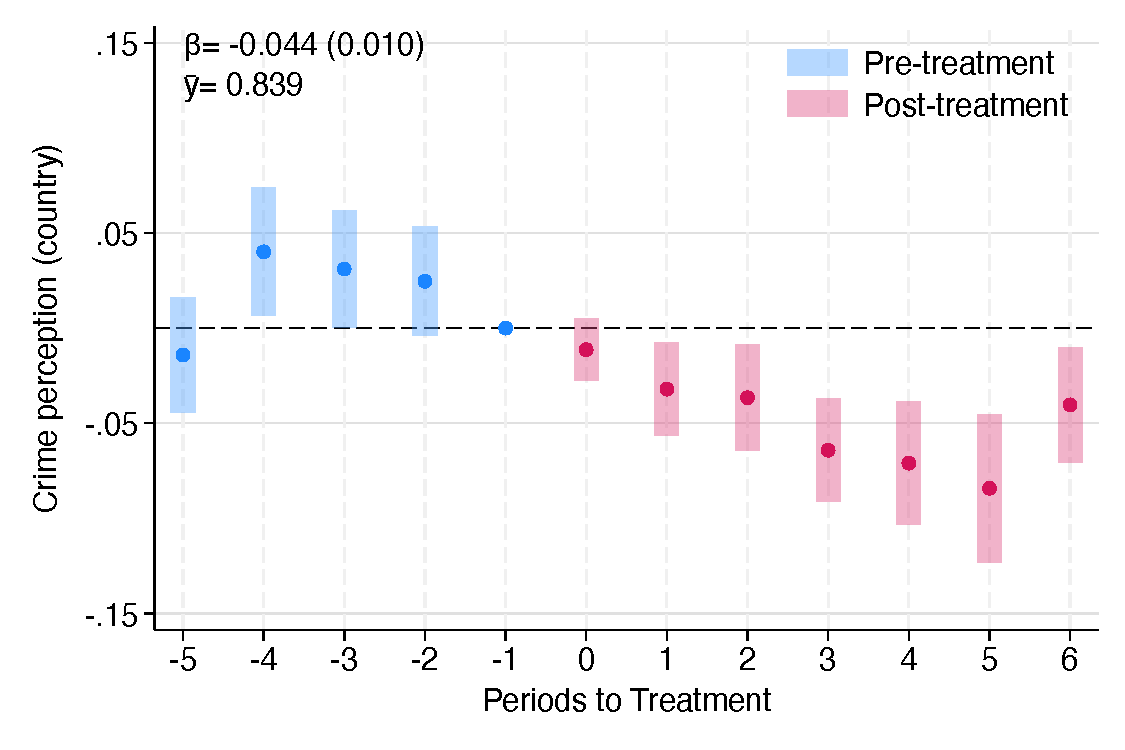
\includegraphics[width=\textwidth]{../manuscript/Graphs/results_perception_country.pdf}
        \caption{In the country}
    \end{subfigure}
    \\[12pt]
    \begin{minipage}{0.99\textwidth}
    \footnotesize Notes: This figure shows the dynamic effects of the \emph{Plan Cuadrante} on the proportion of individuals that perceive an increase in crime in the municipality in the last 12 months (panel a), and on the proportion of individuals that perceive an increase in crime in the country in the last 12 months (panel b). Panel (a) includes 90,696 observations, while panel (b) includes 92,305 observations. The estimation is conducted using the procedure developed in \citet{Callaway} for difference-in-differences with staggered treatment adoption. The dots in the figure represent the estimated coefficients and the bars behind them 95\% confidence intervals. Standard errors are clustered at the municipality level using the wild bootstrapping procedure. The pooled effect and the mean outcome before the introduction of the treatment for every outcome---computed as in Figure \ref{fig:figure02}, using only the pre-treatment observations of treated units---is also presented in each panel.
    \end{minipage}
\end{figure}



 
\clearpage

\subsection{Robustness to the 2010 Earthquake}
\label{sec:earthquake}

The 2010 Maule earthquake could confound our estimates if it differentially affected treated and control municipalities, either by disrupting police operations and thus reducing treatment intensity, or by independently affecting crime perceptions and security outcomes in ways unrelated to \emph{Plan Cuadrante}. To address this concern, we re-estimate our main results excluding municipalities more exposed to the earthquake, defined as those experiencing a Modified Mercalli Intensity greater than 7. This corresponds to 21 municipalities in the ENUSC sample and 158 municipalities in the administrative data sample. The results, reported in Figure \ref{fig:figure02_noEQ}, are nearly identical to the main estimates, confirming that the 2010 earthquake does not drive our findings.

%--- Robustness check: 2010 Maule earthquake (Mercalli > 7 excluded)
\begin{figure}[h!]
    \centering
    \caption{Effects of \emph{Plan Cuadrante} excluding Municipalities Affected by the 2010 Earthquake}
    \label{fig:figure02_noEQ}
    \begin{subfigure}{0.495\textwidth}
        \centering
        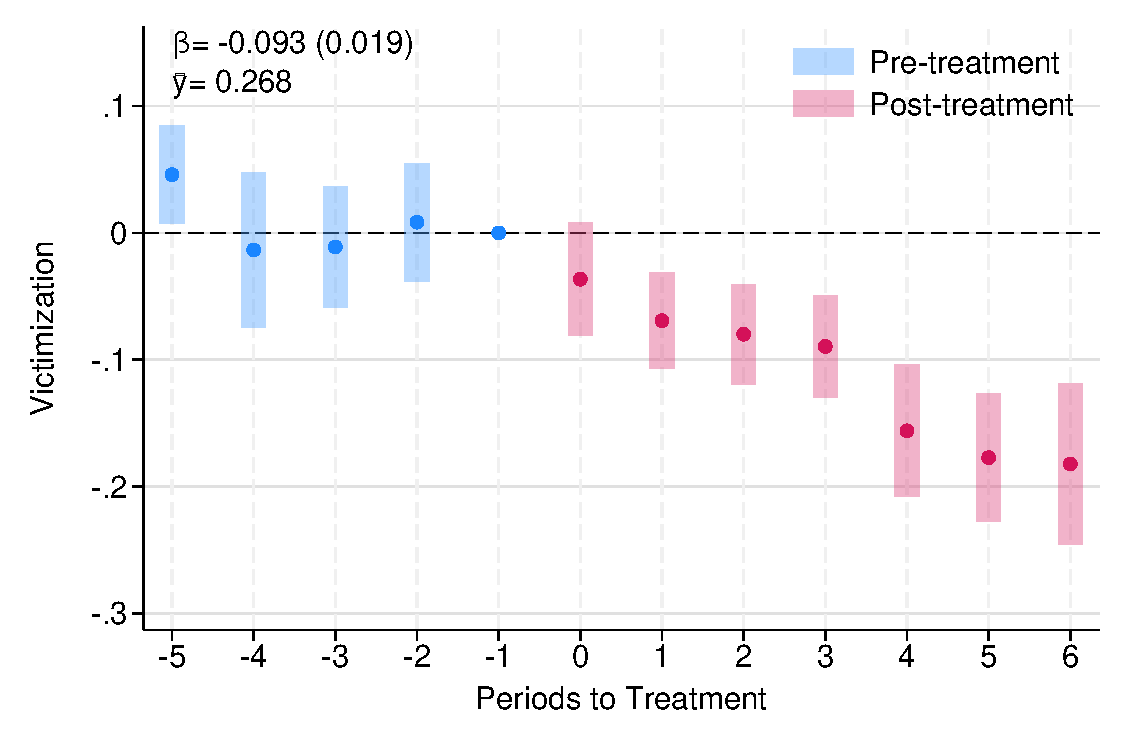
\includegraphics[width=\textwidth]{../manuscript/Graphs/results_victimization_noEQ.pdf}
        \caption{Victimization in last 12 months}
    \end{subfigure}%
    ~
    \begin{subfigure}{0.495\textwidth}
        \centering
        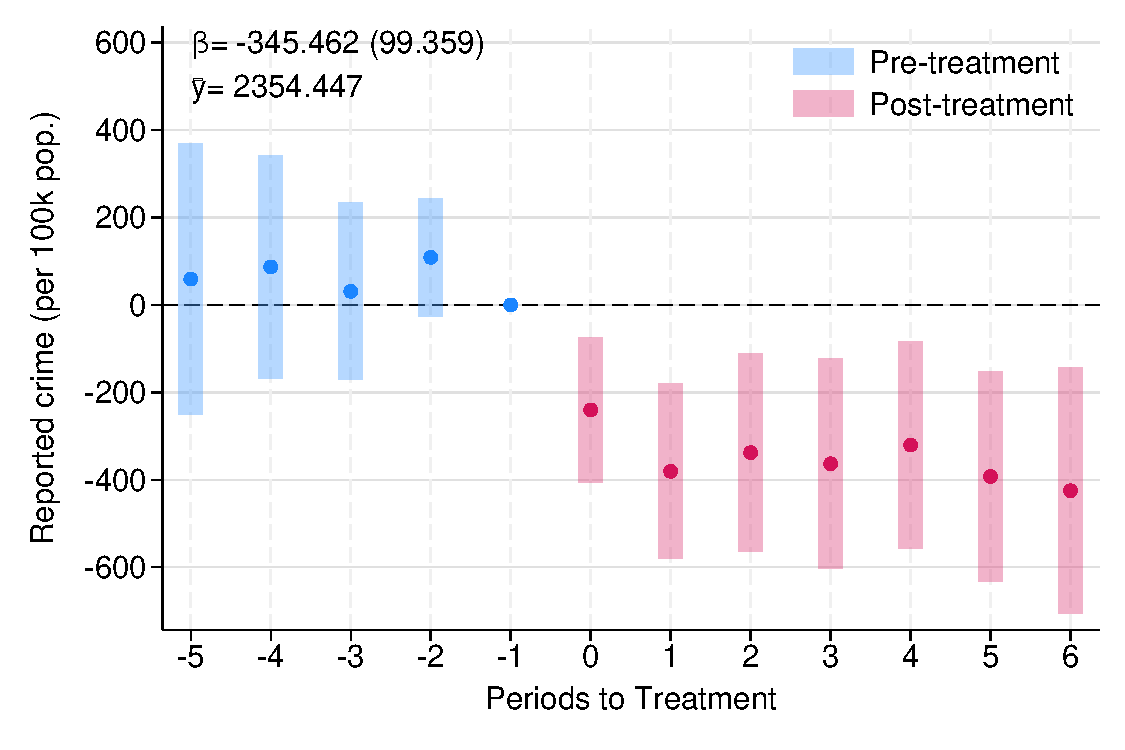
\includegraphics[width=\textwidth]{../manuscript/Graphs/totalreportedcrime_allcomunas_noEQ.pdf}
        \caption{Reported crime per 100k inhabitants}
    \end{subfigure}
    \begin{subfigure}{0.495\textwidth}
        \centering
        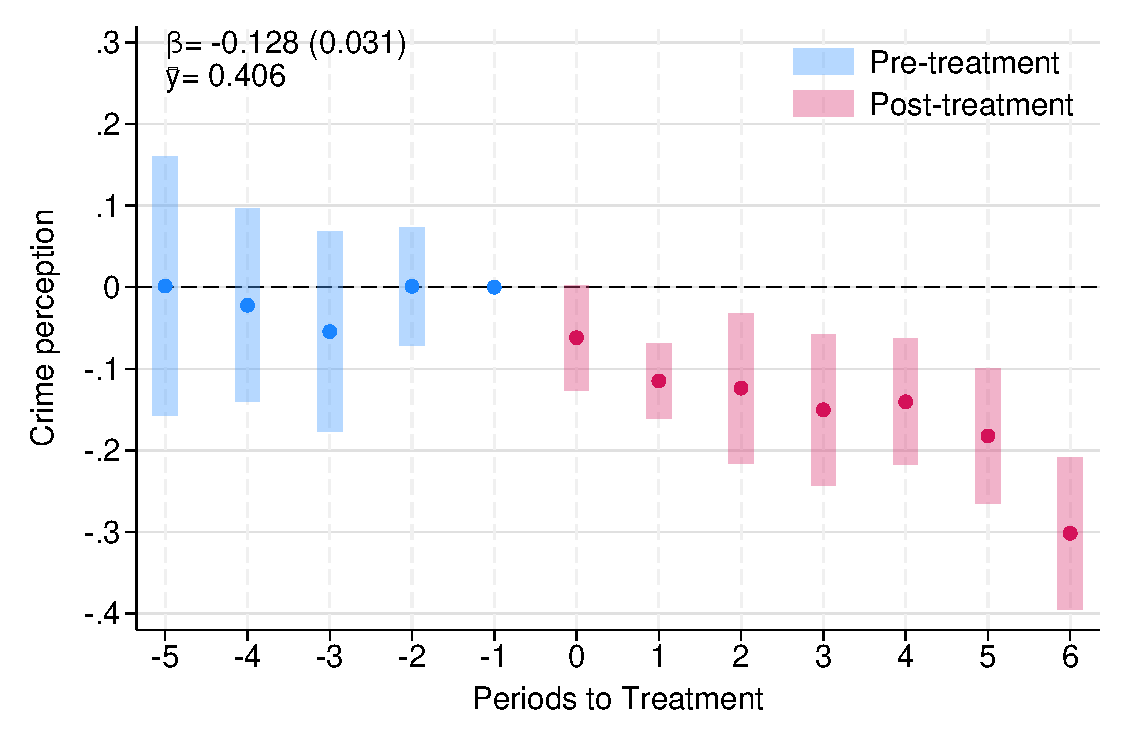
\includegraphics[width=\textwidth]{../manuscript/Graphs/results_perception_noEQ.pdf}
        \caption{Households reporting an increase in crime}
    \end{subfigure}%
    ~
    \begin{subfigure}{0.495\textwidth}
        \centering
        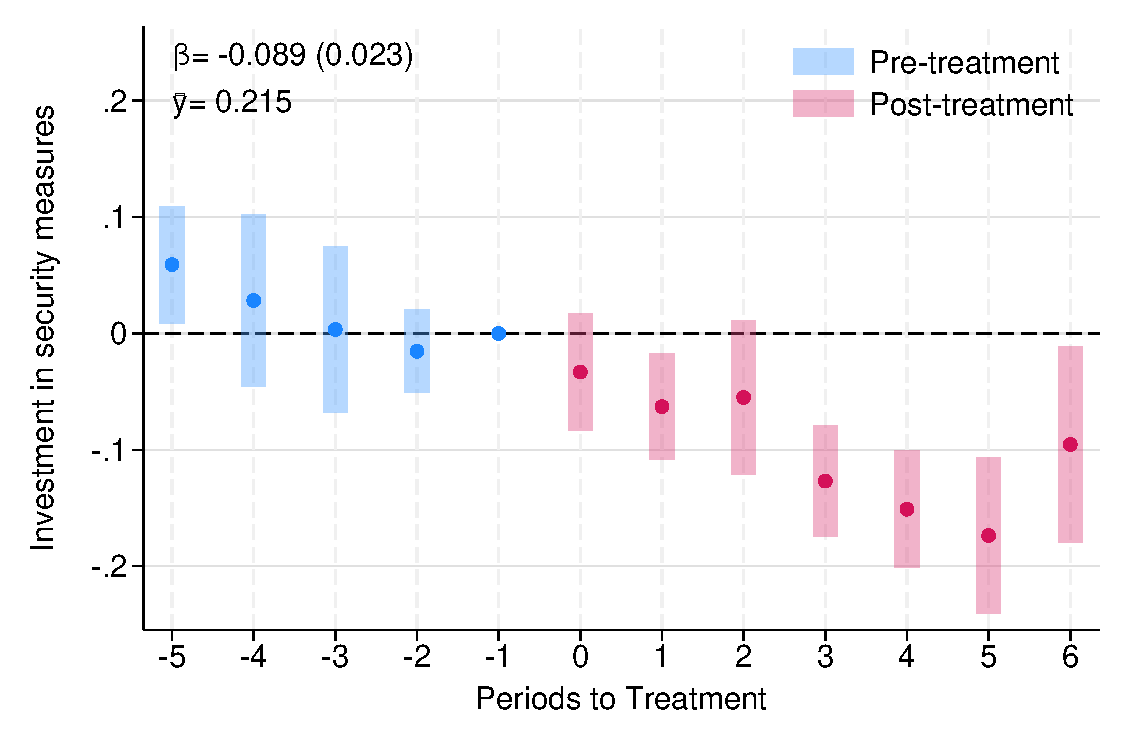
\includegraphics[width=\textwidth]{../manuscript/Graphs/results_hhprotectionmeasures_noEQ.pdf}
        \caption{Households adopting security measures}
    \end{subfigure}
    \\[12pt]
    \begin{minipage}{0.99\textwidth}
    \footnotesize
    Notes: This figure replicates the results of Figure \ref{fig:figure02} after excluding municipalities affected by the 2010 Maule earthquake, defined as those with a Modified Mercalli Intensity (MMI) score strictly greater than 7. The estimation is conducted using the procedure developed in \citet{Callaway} for difference-in-differences with staggered treatment adoption. The dots in the figure represent the estimated coefficients and the bars behind them 95\% confidence intervals. Standard errors are clustered at the municipality level using the wild bootstrapping procedure. The pooled effect and the mean outcome before the introduction of the treatment is also presented in each panel. Panel (a) reports the effect of \emph{Plan Cuadrante} on the probability of household victimization in the last 12 months using the ENUSC survey. Panel (b) reports the effect on the number of crimes reported to the police in the municipality per 100,000 inhabitants using administrative data. Panel (c) reports the effect on the probability of perceiving an increase in crime using the ENUSC survey. Panel (d) reports the effect on the probability of adopting security measures in the last twelve months using the ENUSC survey.
    \end{minipage}
\end{figure}

\clearpage

\subsection{Randomization-Inference Placebo Test}
\label{sec:ri_appendix}

As a further robustness check, we implement a placebo/randomization-inference exercise: we reassign adoption dates and never-treated status at random and re-estimate our specification under the sharp null of no treatment effect for any unit. The estimated direct effect on treated municipalities falls in the bottom first percentile of the resulting placebo distribution, while the analogous estimate for untreated neighbors of treated municipalities falls near its center---between the 40th and 45th percentile---consistent with a genuine effect on treated municipalities and with the absence of spillovers documented in Online Appendix \ref{spillovers} below.

For this exercise, we reassign adoption dates and never-treated status across municipalities $1{,}000$ times and re-estimate the direct and spillover effects under the sharp null, yielding the placebo distributions in Online Appendix Figure~\ref{fig:ri_placebo}. We rely on the estimator of \citet{Chaisemartin} rather than that of \citet{Callaway} for this exercise: re-estimating the latter over a thousand permutations would require prohibitive computational power and running time.

\begin{figure}[h!]
    \centering
    \caption{Randomization Inference for the Direct and Spillover Effects of \emph{Plan Cuadrante}}
    \label{fig:ri_placebo}
    \begin{subfigure}{0.495\textwidth}
        \centering
        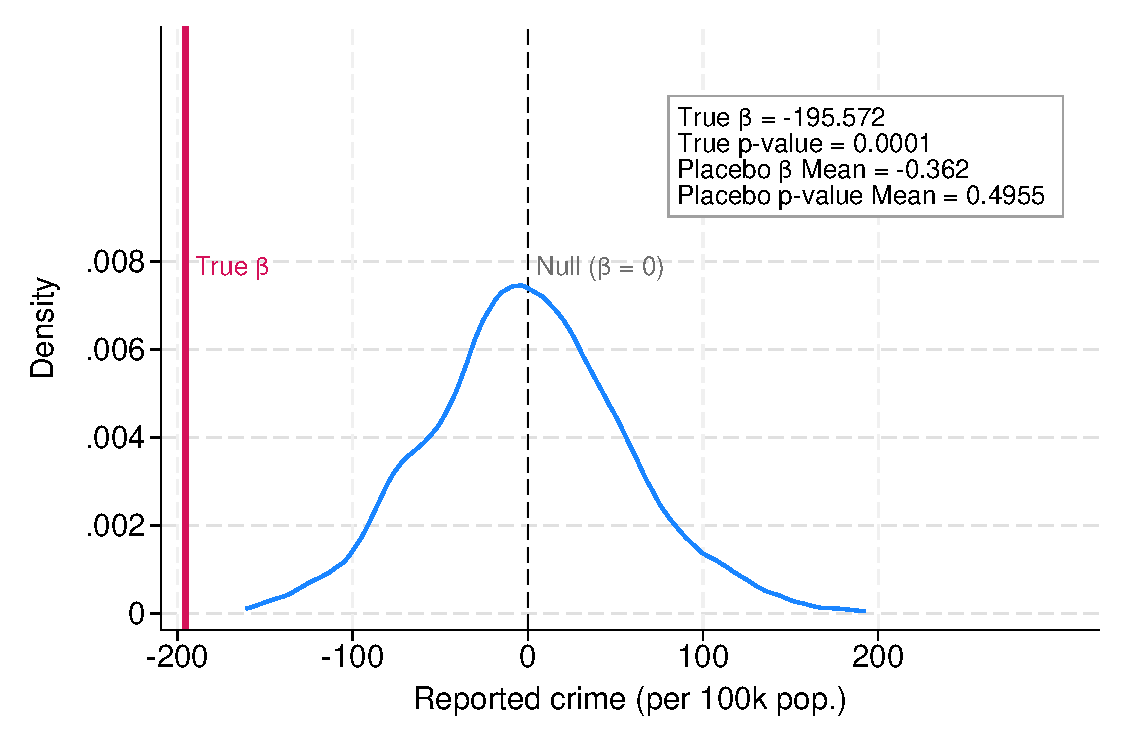
\includegraphics[width=\textwidth]{../manuscript/Graphs/CHDH_RI_placebo_crime.pdf}
        \caption{Reported crime}
        \label{fig:ri_crime}
    \end{subfigure}%
    ~
    \begin{subfigure}{0.495\textwidth}
        \centering
        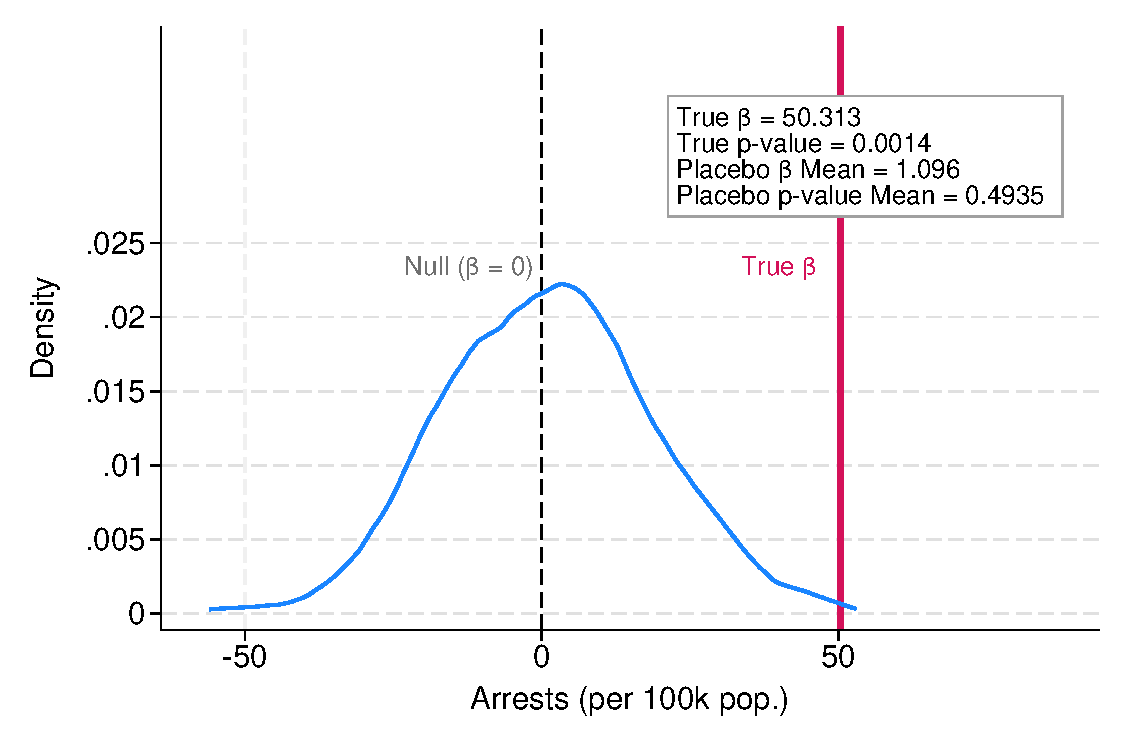
\includegraphics[width=\textwidth]{../manuscript/Graphs/CHDH_RI_placebo_arrests.pdf}
        \caption{Arrests}
        \label{fig:ri_arrests}
    \end{subfigure}

    \begin{subfigure}{0.495\textwidth}
        \centering
        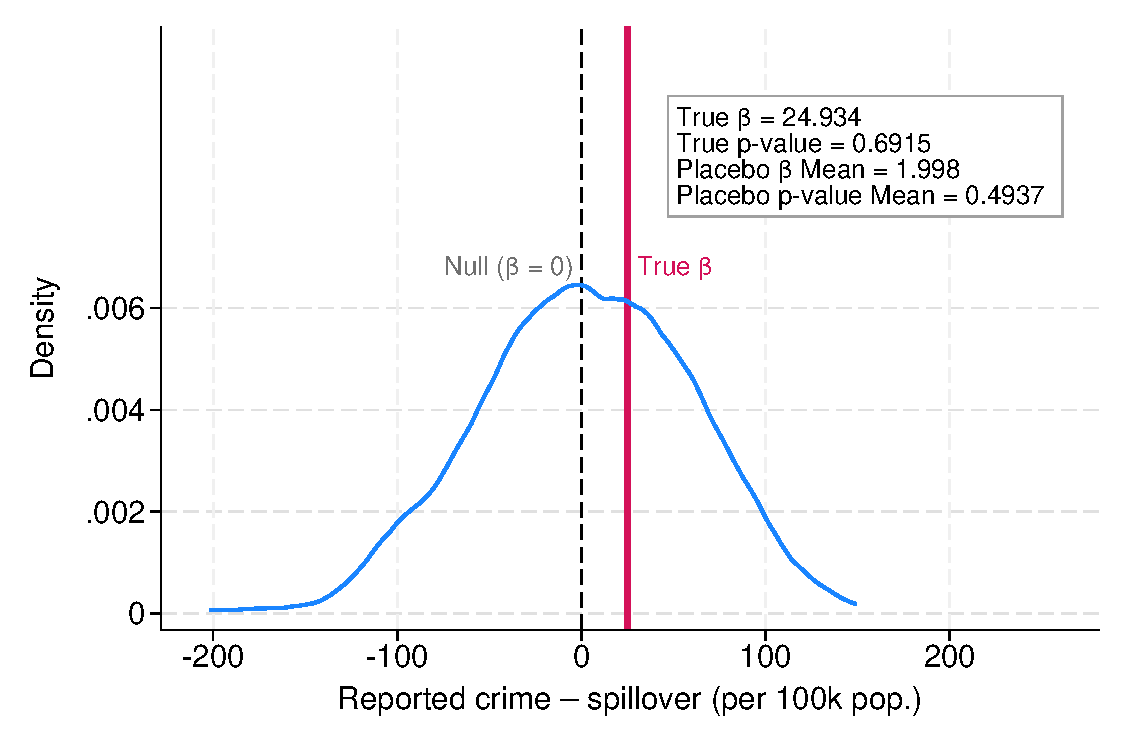
\includegraphics[width=\textwidth]{../manuscript/Graphs/CHDH_RI_placebo_crime_spillover.pdf}
        \caption{Spillovers on Reported crime}
        \label{fig:ri_crime_spillover}
    \end{subfigure}%
    \begin{subfigure}{0.495\textwidth}
        \centering
        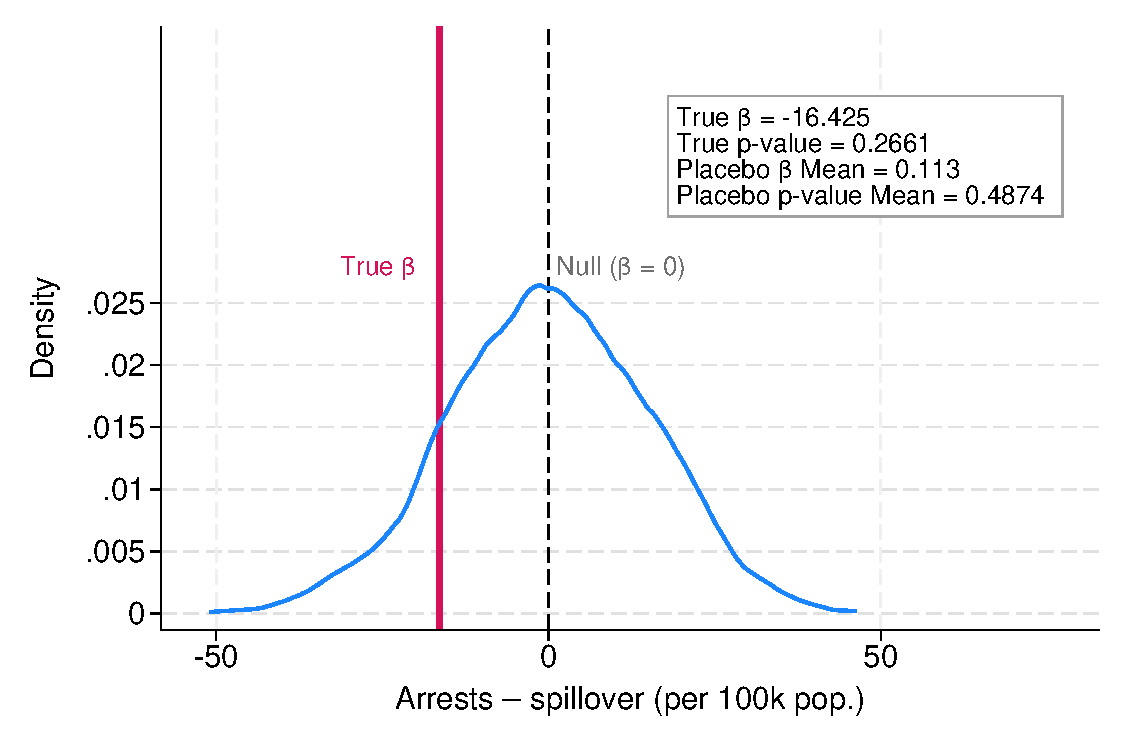
\includegraphics[width=\textwidth]{../manuscript/Graphs/CHDH_RI_placebo_arrests_spillover.pdf}
        \caption{Spillovers on Arrests}
        \label{fig:ri_arrests_spillover}
    \end{subfigure}
    \begin{minipage}{0.95\textwidth}
    \footnotesize
    Notes: This figure presents randomization inference results under the sharp null of no treatment effect, using the heterogeneity-robust estimator of \citet{Chaisemartin}. Each curve is the kernel density of 1{,}000 placebo ATT estimates obtained by jointly permuting \emph{Plan Cuadrante} adoption dates and never-treated status across municipalities (drawing from the empirical distribution of (date, status) pairs, so the marginal counts of treated and never-treated municipalities are preserved in every permutation). In each permutation the variable PC is shuffled across all 346 municipalities and a new time-varying treatment indicator is computed before re-estimating the dynamic effects. The solid colored vertical line marks the point estimate from the true rollout; the dashed black line marks the null expectation $\beta = 0$. The boxes report the true point estimate, its asymptotic two-sided $p$-value, and the mean of the placebo $\beta$ and placebo $p$-value distributions.
    \end{minipage}
\end{figure}

\clearpage

\subsection{Testing for Spatial Spillovers}
\label{spillovers}

This Online Appendix details the specifications behind the spillover tests summarized in Section~\ref{sec:spillovers}.

For the intensity-based test in the spirit of \citet{crepon2013}, we replace the binary neighbor-treatment indicator with a continuous measure of exposure and restrict the sample to never-treated municipalities,
\begin{equation}
Outcome_{mt}= \delta_{1}\,\mbox{\textit{Share neighbors with Plan Cuadrante}}_{mt} + Municipality_{m} + Year_{t} + u_{mt}
\label{eq:crepon}
\end{equation}
\noindent Because the treatment is continuous, we estimate it with the heterogeneity-robust estimator of \citet{Chaisemartin}, measuring exposure both as the share of treated neighbors (Online Appendix Figure~\ref{fig:figure_continuous_spillovers}) and as their number (Online Appendix Figure~\ref{fig:figure_count_spillovers}).

The baseline test estimates the effect of \emph{Plan Cuadrante} on reported crime, arrests, police officers, and patrol vehicles in neighboring untreated municipalities,
\begin{equation}
Outcome_{mt}= \delta_{1}\,\mbox{\textit{Plan Cuadrante near municip.}}_{mt} + Municipality_{m} + Year_{t} + u_{mt}
\label{eq:main3}
\end{equation}
\noindent where the sample is restricted to municipalities that never adopted the program, each is assigned a treatment date equal to the earliest adoption among its treated neighbors, and $\delta_{1}$ is estimated dynamically with the staggered difference-in-differences estimator of \citet{Callaway}. Because these administrative outcomes are observed for every municipality, we estimate the specification on the full national sample (Online Appendix Figure~\ref{fig:spillover_admin}).

Finally, we re-estimate the baseline administrative specification on the municipalities neighboring the 46 ENUSC municipalities (Online Appendix Figure~\ref{fig:figure_46ENUSC_spillovers_admin}); and, for the outcomes measured only in ENUSC, we estimate the spillover of early-adopting ENUSC municipalities on their late-adopting ENUSC neighbors before the latter's own adoption (Online Appendix Figure~\ref{fig:figure_results_spillovers_enusc}). The six focal late-adopters, each shown with its earliest-adopting ENUSC neighbor and that neighbor's adoption year, are Molina (Curic\'o, 2005), Tocopilla (Iquique, 2005), San Carlos (Chill\'an, 2007), Padre Hurtado (Pe\~naflor, 2008), Calera (Quillota, 2008), and Limache (Quillota, 2008). Across all of these specifications, the estimated spillover effects are small and statistically indistinguishable from zero.

\begin{figure}[h!]
    \centering
    \caption{Geographic Spillovers of \emph{Plan Cuadrante} by Share of Treated Neighbors}
    \label{fig:figure_continuous_spillovers}
    \begin{subfigure}{0.495\textwidth}
        \centering
        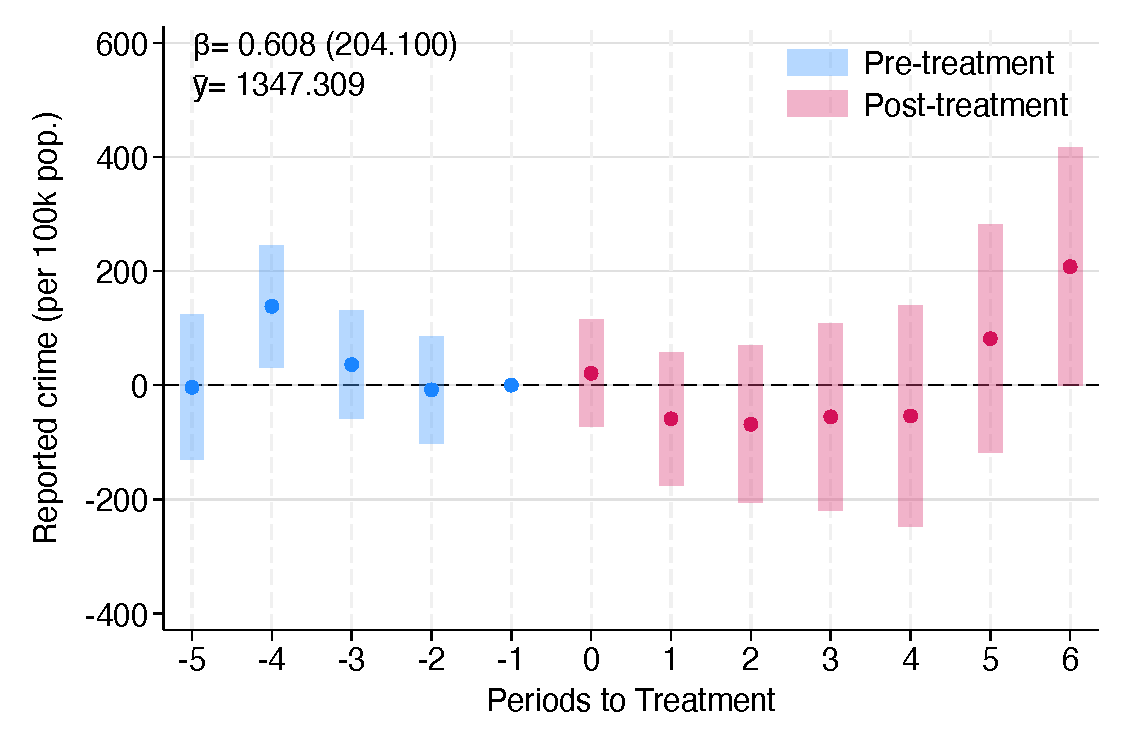
\includegraphics[width=0.98\textwidth]{../manuscript/Graphs/CHDH_continuous_spillover_crime.pdf}
        \caption{Spillovers on Reported Crime}
    \end{subfigure}%
    ~
    \begin{subfigure}{0.495\textwidth}
        \centering
        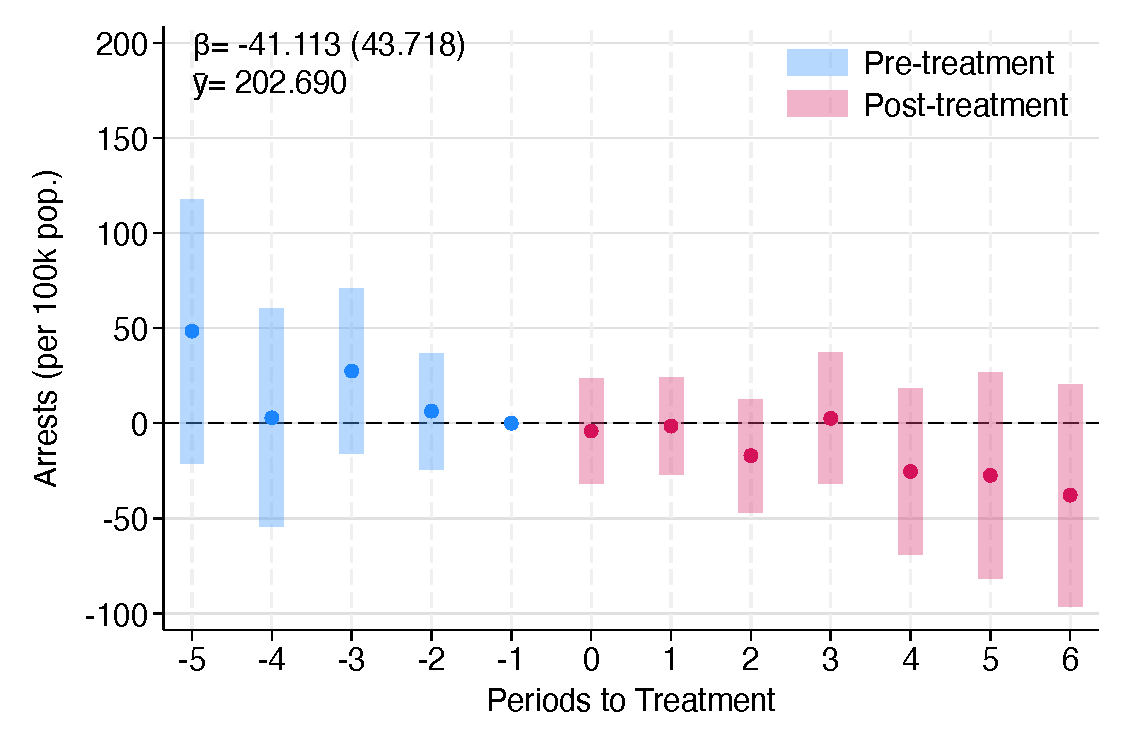
\includegraphics[width=0.98\textwidth]{../manuscript/Graphs/CHDH_continuous_spillover_arrests.pdf}
        \caption{Spillovers on Arrests}
    \end{subfigure}

    \vspace{0.5em}

    \begin{subfigure}{0.495\textwidth}
        \centering
        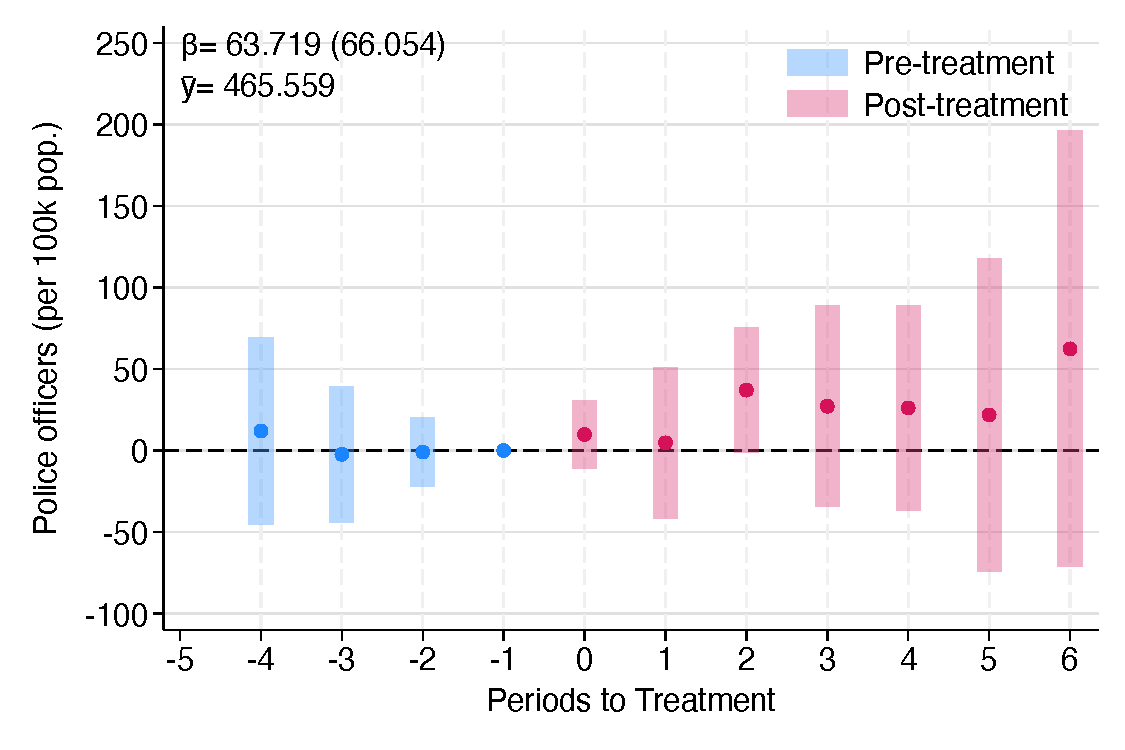
\includegraphics[width=0.98\textwidth]{../manuscript/Graphs/CHDH_continuous_spillover_dotpc.pdf}
        \caption{Spillovers on Police Officers}
    \end{subfigure}%
    ~
    \begin{subfigure}{0.495\textwidth}
        \centering
        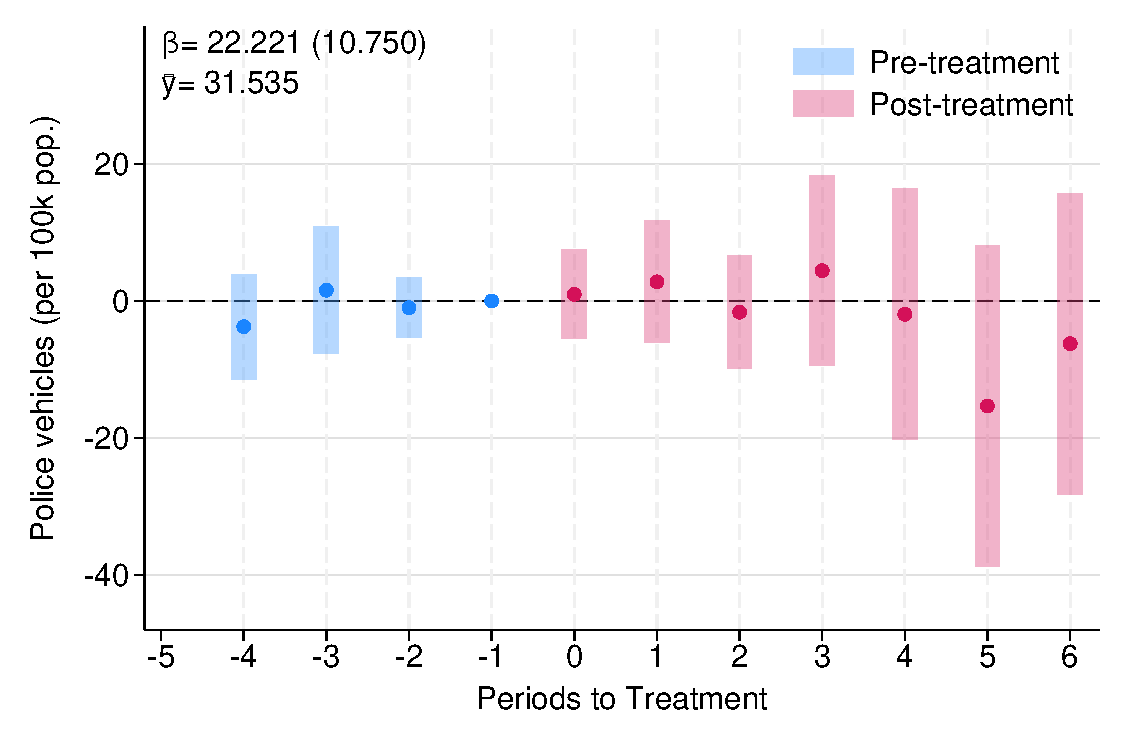
\includegraphics[width=0.98\textwidth]{../manuscript/Graphs/CHDH_continuous_spillover_vehiclespc.pdf}
        \caption{Spillovers on Patrol Vehicles}
    \end{subfigure}

    \begin{minipage}{0.95\textwidth}
    \footnotesize
    Notes: This figure reports the geographic spillover effects of \emph{Plan Cuadrante} on four outcomes for never-treated municipalities: reported crime per 100,000 inhabitants (panel a), arrests per 100,000 inhabitants (panel b), the number of police officers per 100,000 inhabitants (panel c), and the number of patrol vehicles per 100,000 inhabitants (panel d). Unlike the dummy spillover specification, the treatment variable is now continuous and equals the share of neighboring municipalities that have implemented \emph{Plan Cuadrante} by year $t$, following the spillover-intensity approach of \citet{crepon2013}. The sample is restricted to municipalities that never adopted \emph{Plan Cuadrante}. Estimation is performed using the heterogeneity-robust estimator of \citet{Chaisemartin}, which accommodates a continuous, time-varying treatment intensity in a staggered design. The dots represent the estimated dynamic effects and the bars behind them denote 95\% confidence intervals. Standard errors are clustered at the municipality level. The pooled effect  and the mean of the outcome among municipalities with no treated neighbors are reported in each panel.
    \end{minipage}
\end{figure}


\begin{figure}[h!]
    \centering
    \caption{Geographic Spillovers of \emph{Plan Cuadrante} by Number of Treated Neighbors}
    \label{fig:figure_count_spillovers}
    \begin{subfigure}{0.495\textwidth}
        \centering
        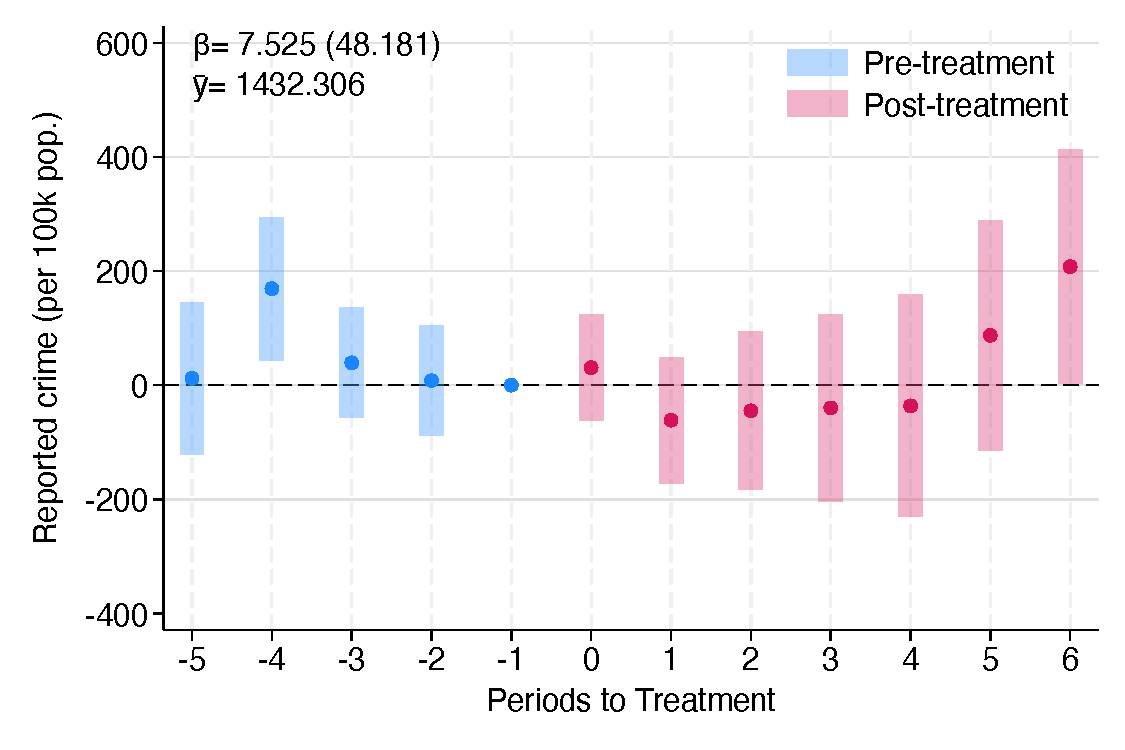
\includegraphics[width=0.98\textwidth]{../manuscript/Graphs/CHDH_continuous_spillover_crime_count.pdf}
        \caption{Spillovers on Reported Crime}
    \end{subfigure}%
    ~
    \begin{subfigure}{0.495\textwidth}
        \centering
        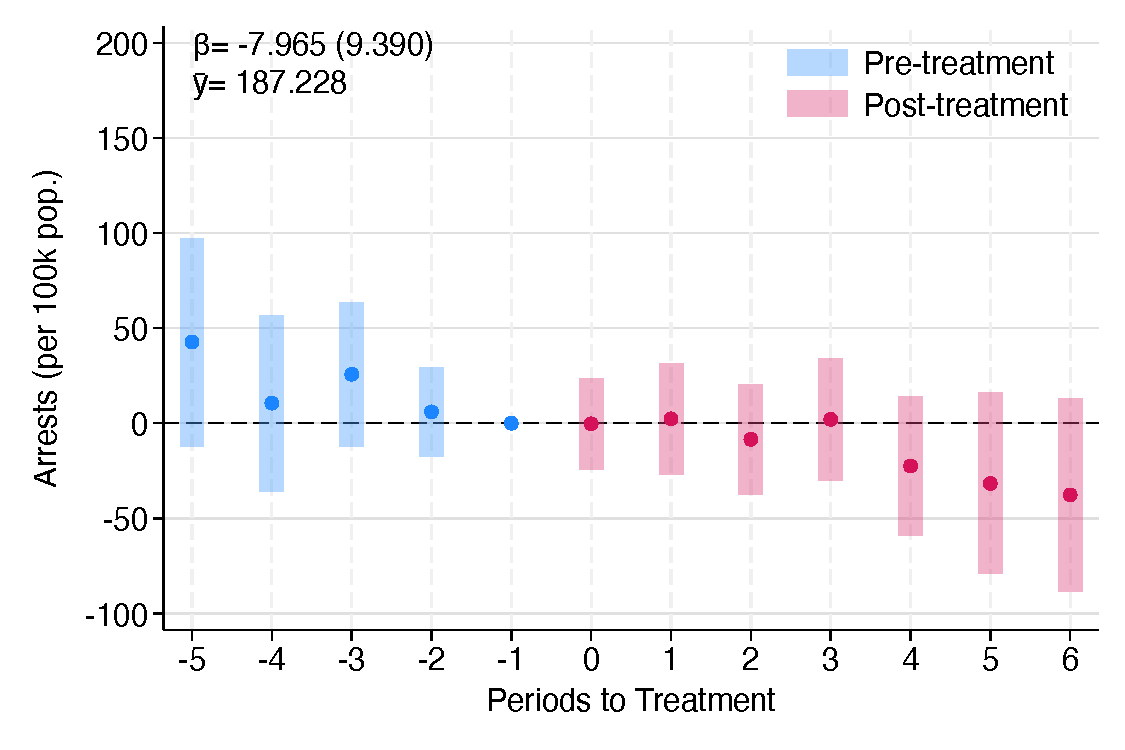
\includegraphics[width=0.98\textwidth]{../manuscript/Graphs/CHDH_continuous_spillover_arrests_count.pdf}
        \caption{Spillovers on Arrests}
    \end{subfigure}

    \vspace{0.5em}

    \begin{subfigure}{0.495\textwidth}
        \centering
        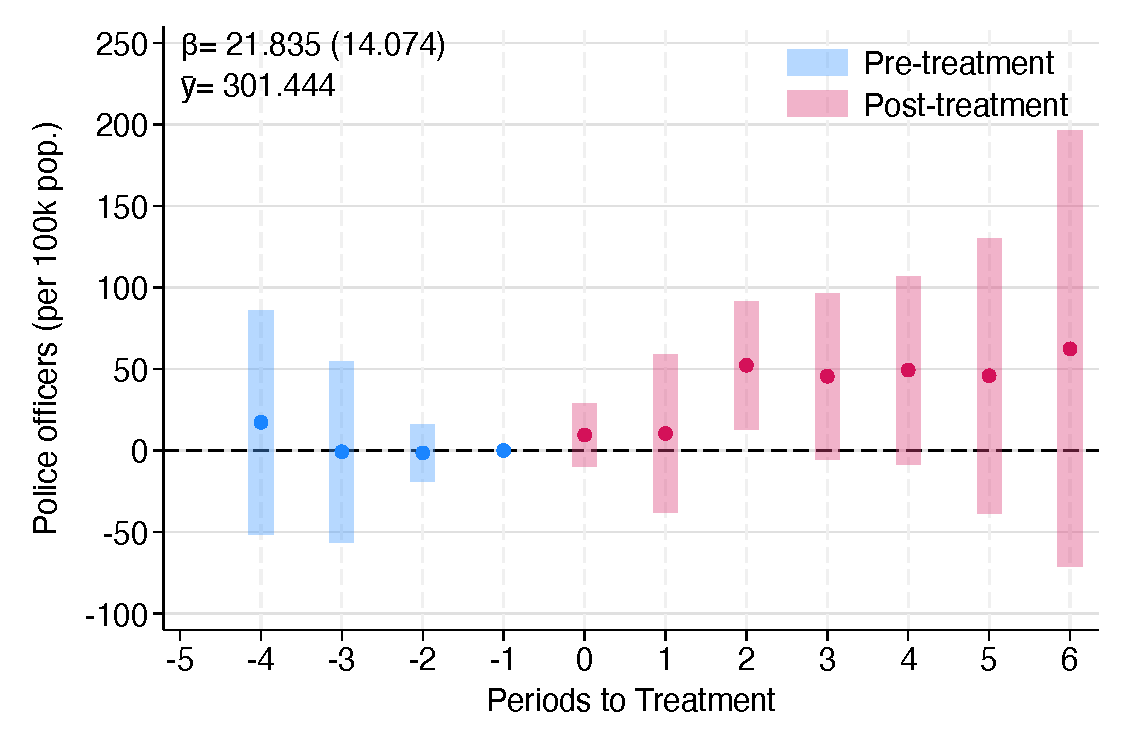
\includegraphics[width=0.98\textwidth]{../manuscript/Graphs/CHDH_continuous_spillover_dotpc_count.pdf}
        \caption{Spillovers on Police Officers}
    \end{subfigure}%
    ~
    \begin{subfigure}{0.495\textwidth}
        \centering
        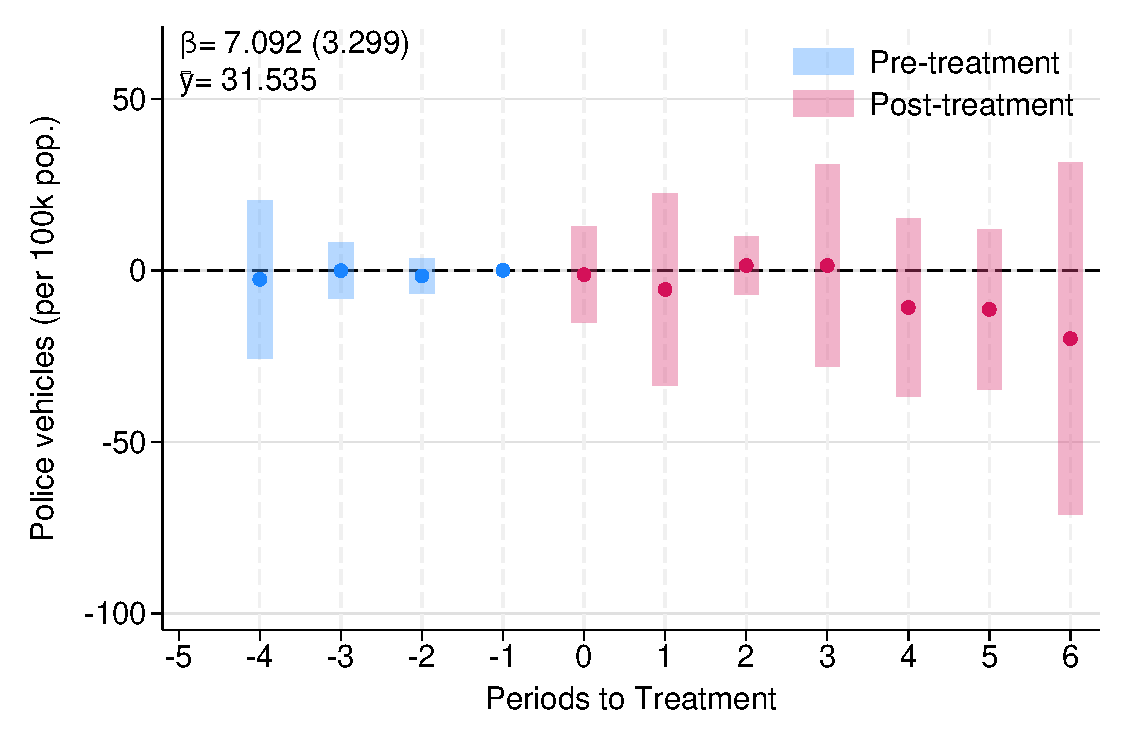
\includegraphics[width=0.98\textwidth]{../manuscript/Graphs/CHDH_continuous_spillover_vehiclespc_count.pdf}
        \caption{Spillovers on Patrol Vehicles}
    \end{subfigure}

    \begin{minipage}{0.95\textwidth}
    \footnotesize
    Notes: This figure reports the geographic spillover effects of \emph{Plan Cuadrante} on four outcomes for never-treated municipalities: reported crime per 100,000 inhabitants (panel a), arrests per 100,000 inhabitants (panel b), the number of police officers per 100,000 inhabitants (panel c), and the number of patrol vehicles per 100,000 inhabitants (panel d). Unlike the dummy spillover specification, the treatment variable is now continuous and equals the number of neighboring municipalities that have implemented \emph{Plan Cuadrante} by year $t$, following the spillover-intensity approach of \citet{crepon2013}. The sample is restricted to municipalities that never adopted \emph{Plan Cuadrante}. Estimation is performed using the heterogeneity-robust estimator of \citet{Chaisemartin}, which accommodates a continuous, time-varying treatment intensity in a staggered design. The dots represent the estimated dynamic effects and the bars behind them denote 95\% confidence intervals. Standard errors are clustered at the municipality level. The pooled effect  and the mean of the outcome among municipalities with no treated neighbors are reported in each panel.
    \end{minipage}
\end{figure}

\clearpage

%--- Implementation
\begin{figure}[h!]
    \centering
    \caption{Geographic Spillovers of \emph{Plan Cuadrante} on Neighboring Untreated Municipalities}
    \label{fig:spillover_admin}
    \begin{subfigure}{0.495\textwidth}
        \centering
        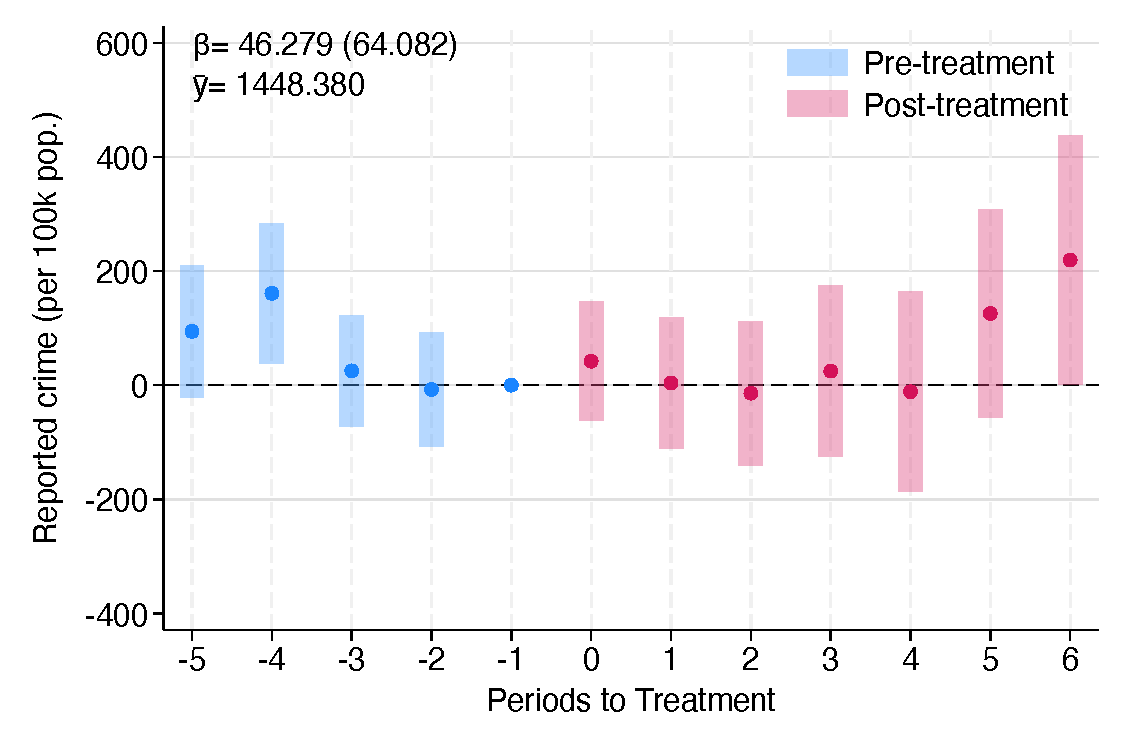
\includegraphics[width=0.98\textwidth]{../manuscript/Graphs/totalreportedcrime_allcomunas_neighbors.pdf}
        \caption{Spillovers on Reported crime}
    \end{subfigure}%
    ~ 
    \begin{subfigure}{0.495\textwidth}
    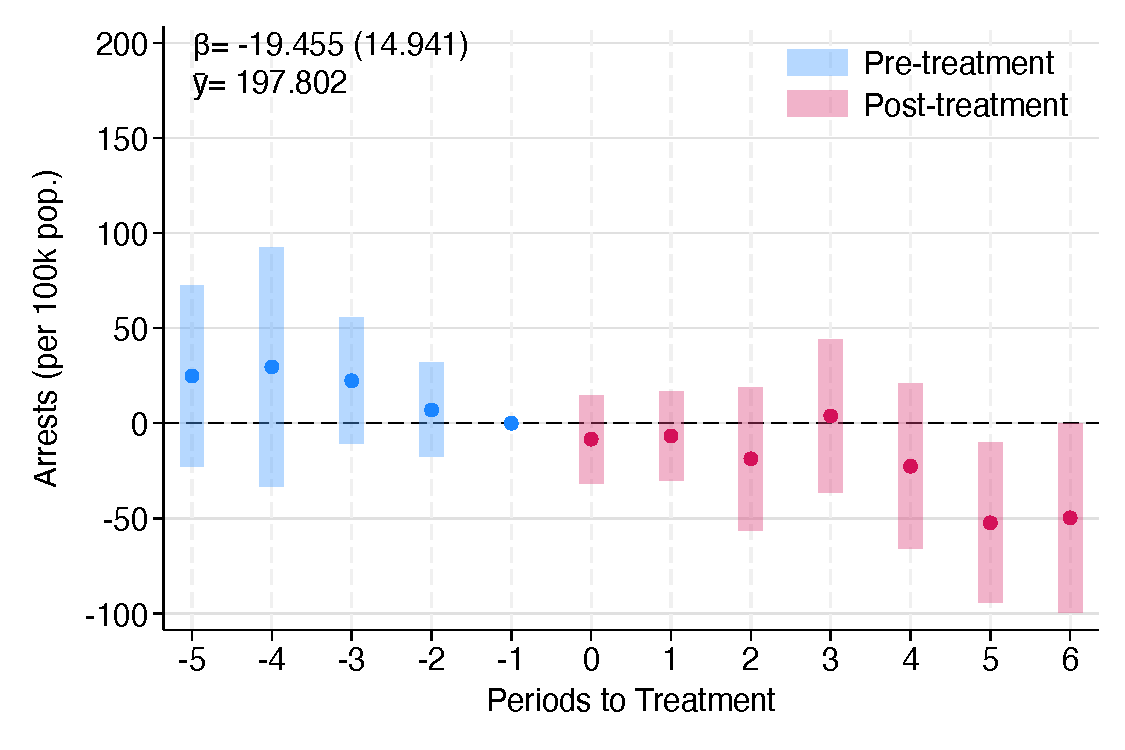
\includegraphics[width=0.98\textwidth]{../manuscript/Graphs/totalarrestscrime_allcomunas_neighbors.pdf}
        \caption{Spillovers on Arrests}
    \end{subfigure}
    \begin{subfigure}{0.495\textwidth}
        \centering
        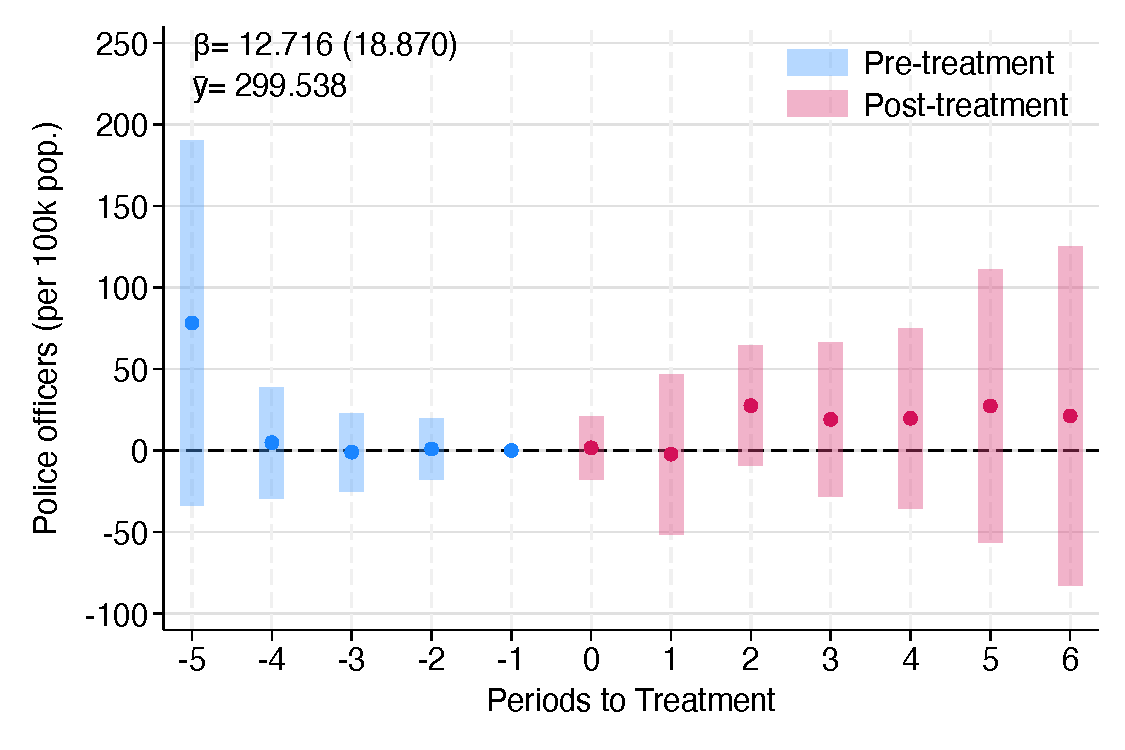
\includegraphics[width=0.98\textwidth]{../manuscript/Graphs/dotpc_allcomunas_neighbors.pdf}
        \caption{Spillovers on Police Officers}
    \end{subfigure}%
    ~ 
    \begin{subfigure}{0.495\textwidth}
    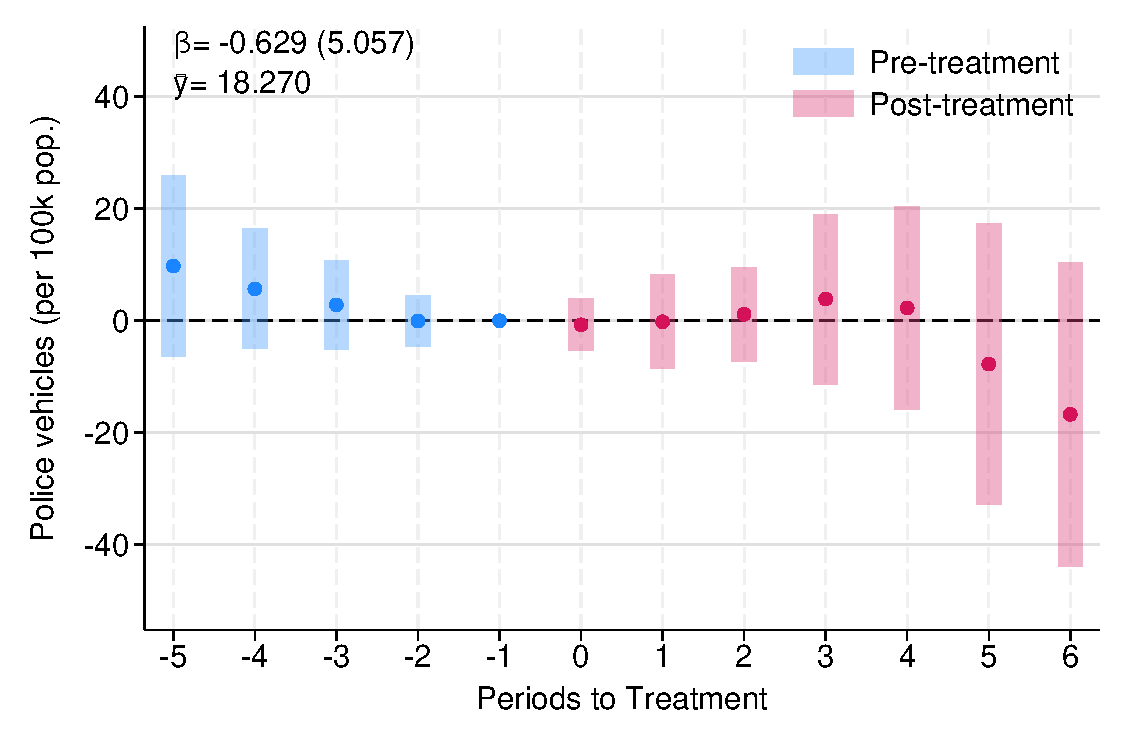
\includegraphics[width=0.98\textwidth]{../manuscript/Graphs/vehiclespc_allcomunas_neighbors.pdf}
        \caption{Spillovers on Patrol Vehicles}
    \end{subfigure}
    \begin{minipage}{0.9\textwidth}
    \footnotesize
    Notes: This figure reports the spillover effects of \emph{Plan Cuadrante} on the number of crimes reported to the police in the municipality per 100,000 inhabitants (panel a), the number of arrests in the municipality per 100,000 inhabitants (panel b), the number of police officers per 100,000 inhabitants (panel c), and the number of patrol vehicles per 100,000 inhabitants (panel d). Panels (a)--(d) include 2,859, 2,166, 1,144, and 1,942 observations respectively. Specifically, the figure shows the dynamic effects of the \emph{Plan Cuadrante} for neighbor municipalities which never introduced the program. The estimation is conducted using the procedure developed in \citet{Callaway} for difference-in-differences with staggered treatment adoption, using as the treatment introduction date the earliest date of a neighboring municipality. The dots in the figure represent the estimated coefficients and the bars behind them 95\% confidence intervals. Standard errors are clustered at the municipality level using the wild bootstrapping procedure. The pooled effect and the mean outcome before the introduction of the treatment for every outcome is also presented in each panel. 
    \end{minipage}
\end{figure}

\clearpage

\begin{figure}[h!]
    \centering
    \caption{Geographic Spillovers of \emph{Plan Cuadrante} for Neighbors of the ENUSC Municipalities (Administrative Outcomes)}
    \label{fig:figure_46ENUSC_spillovers_admin}
    \begin{subfigure}{0.495\textwidth}
        \centering
        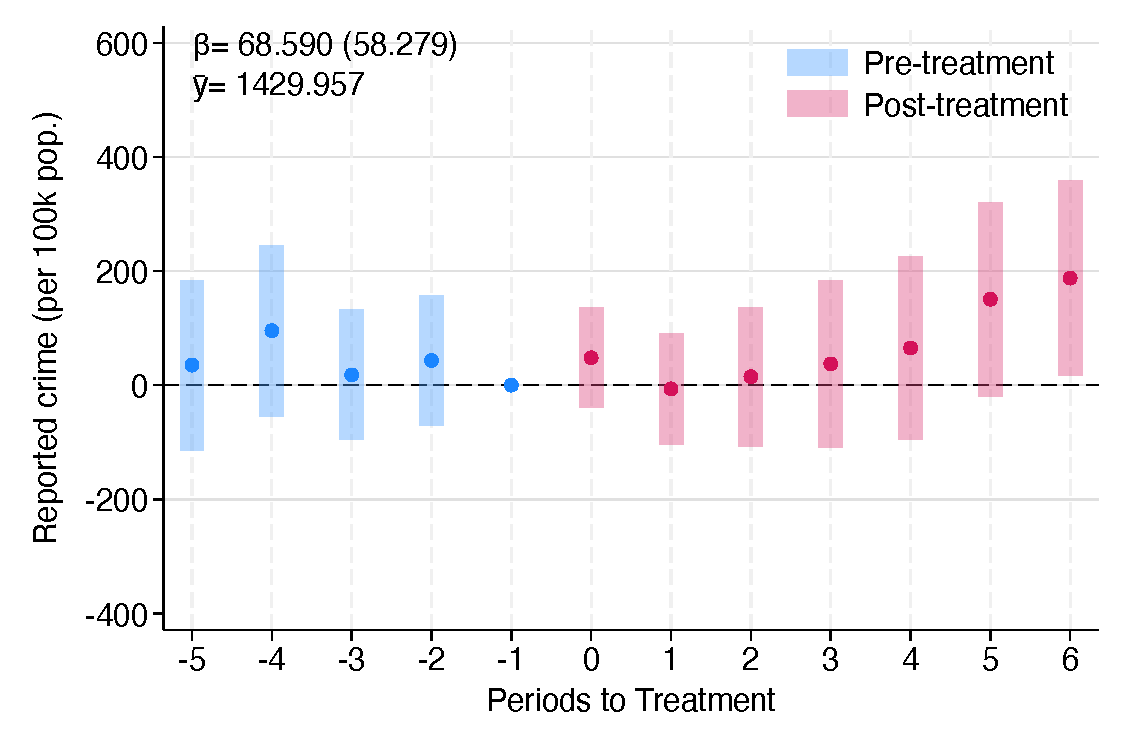
\includegraphics[width=0.98\textwidth]{../manuscript/Graphs/totalreportedcrime_enusc47_neighbors.pdf}
        \caption{Spillovers on Reported Crime}
    \end{subfigure}%
    ~
    \begin{subfigure}{0.495\textwidth}
        \centering
        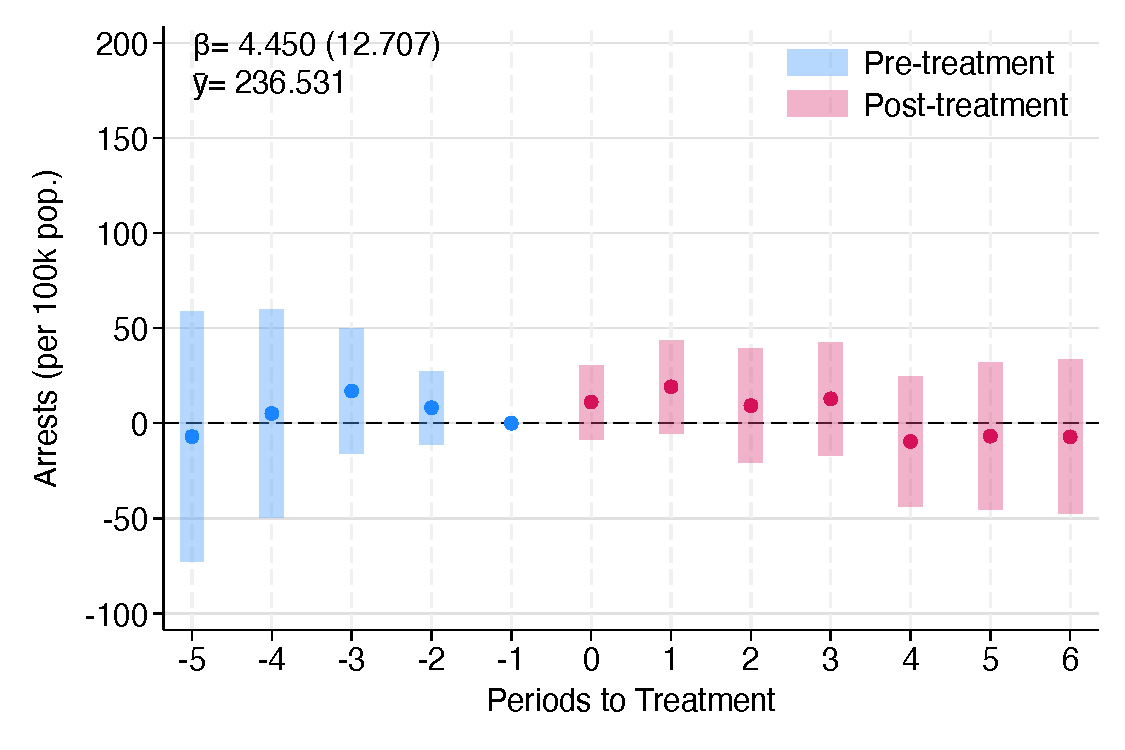
\includegraphics[width=0.98\textwidth]{../manuscript/Graphs/totalarrestscrime_enusc47_neighbors.pdf}
        \caption{Spillovers on Arrests}
    \end{subfigure}

    \vspace{0.5em}

    \begin{subfigure}{0.495\textwidth}
        \centering
        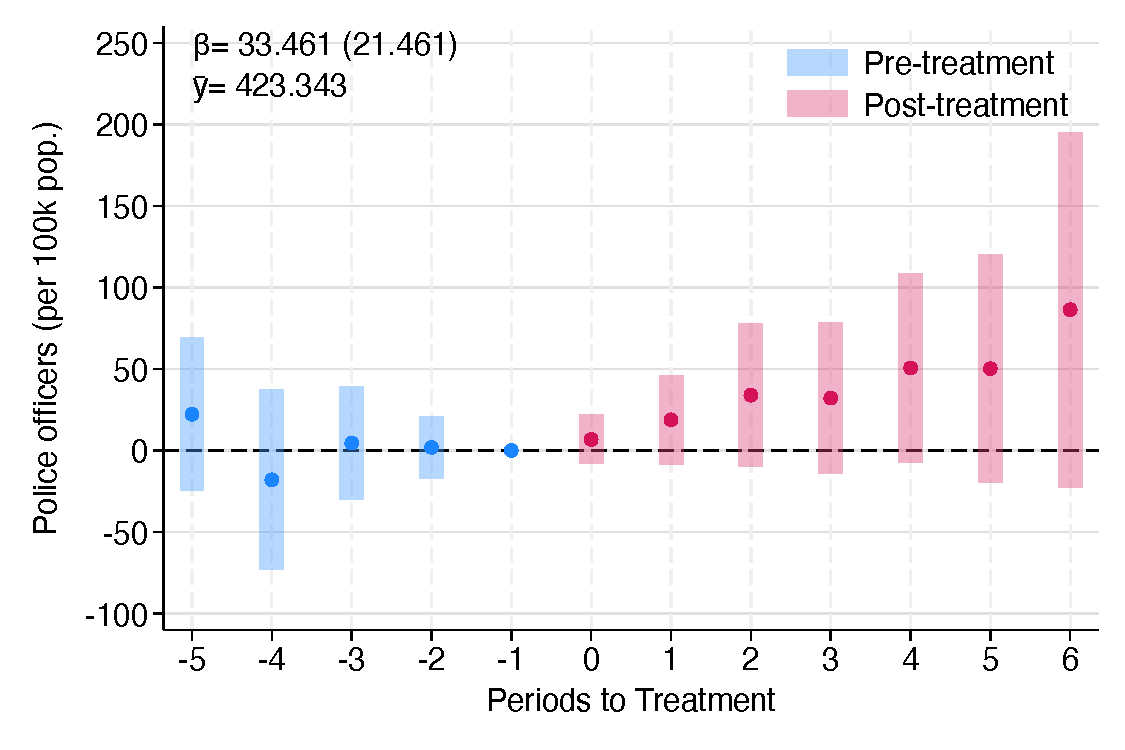
\includegraphics[width=0.98\textwidth]{../manuscript/Graphs/dotpc_enusc47_neighbors.pdf}
        \caption{Spillovers on Police Officers}
    \end{subfigure}%
    ~
    \begin{subfigure}{0.495\textwidth}
        \centering
        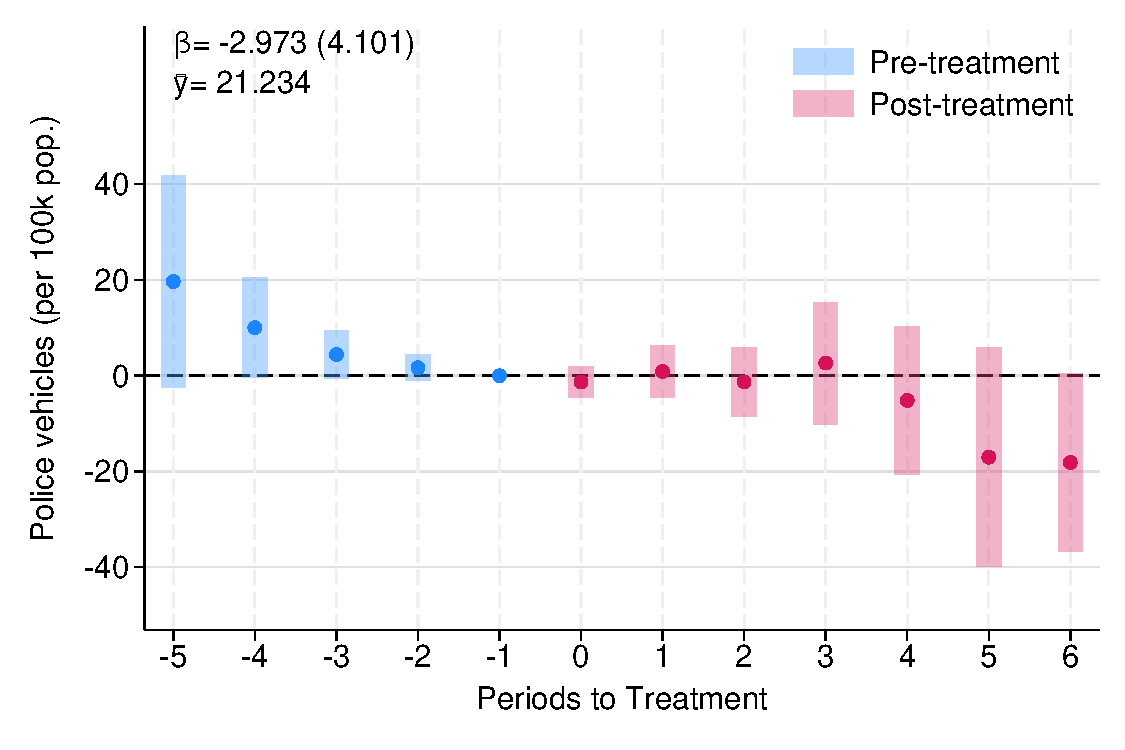
\includegraphics[width=0.98\textwidth]{../manuscript/Graphs/vehiclespc_enusc47_neighbors.pdf}
        \caption{Spillovers on Patrol Vehicles}
    \end{subfigure}

\begin{minipage}{\textwidth}
\footnotesize Notes: This figure reports the spillover effects of \emph{Plan Cuadrante} on the number of crimes reported to the police in the municipality per 100,000 inhabitants (panel a), on the number of arrests in the municipality per 100,000 inhabitants (panel b), on the number of police officers (panel c), and on the number of patrol vehicles (panel d). Specifically, the figure shows the dynamic effects of \emph{Plan Cuadrante} for neighboring never-treated municipalities to the 46 municipalities included in the ENUSC sample. The estimation is conducted using the procedure developed in \citet{Callaway} for difference-in-differences with staggered treatment adoption, using as the treatment introduction date the earliest date of a neighboring municipality. The dots in the figure represent the estimated coefficients and the bars behind them 95\% confidence intervals. Standard errors are clustered at the municipality level using the wild bootstrap procedure. The pooled effect and the mean outcome before the introduction of the treatment for each outcome are also presented in each panel.
\end{minipage}
\end{figure}


\begin{figure}[h!]
    \centering
    \caption{Geographic Spillovers of \emph{Plan Cuadrante} on ENUSC Survey Outcomes (Early- to Late-Adopting Municipalities)}
    \label{fig:figure_results_spillovers_enusc}
    \begin{subfigure}{0.495\textwidth}
        \centering
        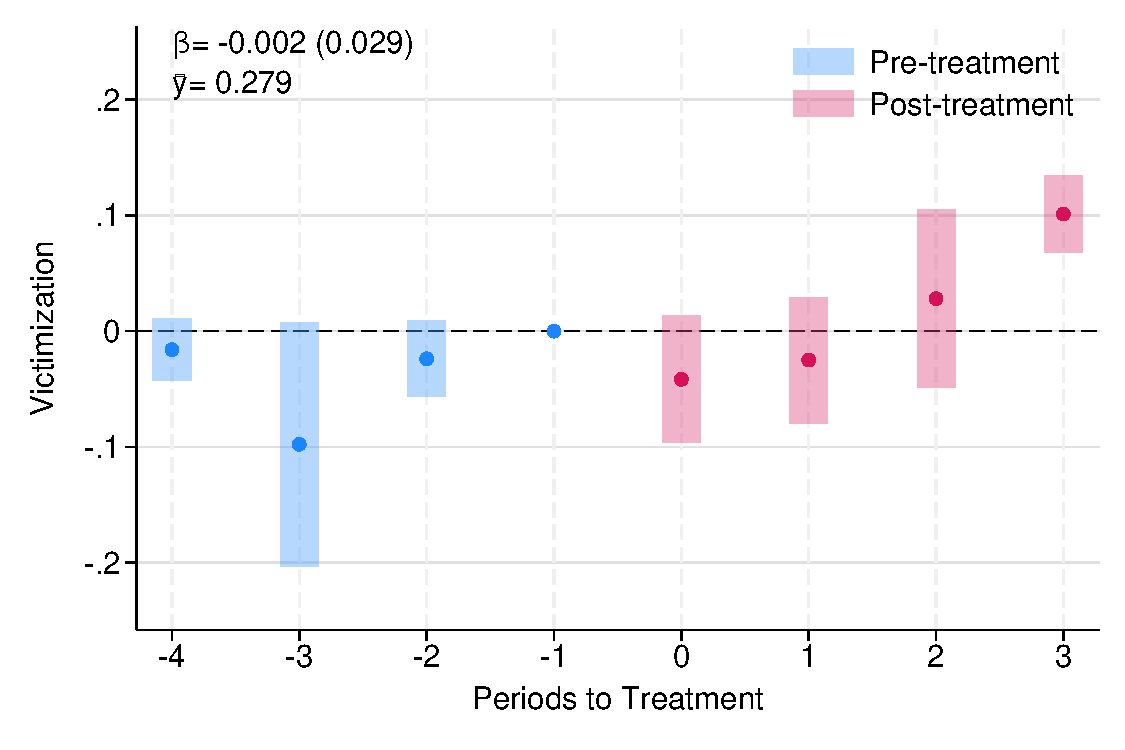
\includegraphics[width=0.98\textwidth]{../manuscript/Graphs/results_spillover_delitos.pdf}
        \caption{Spillovers on Victimization in last 12 months}
    \end{subfigure}%
    ~
    \begin{subfigure}{0.495\textwidth}
        \centering
        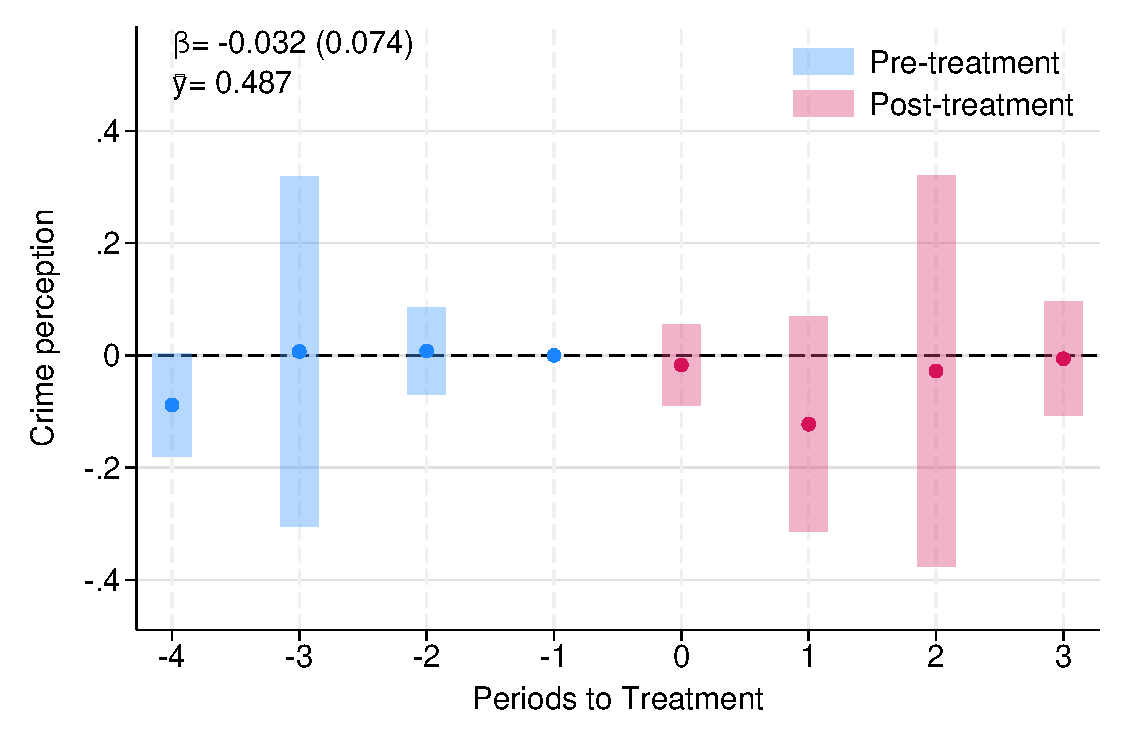
\includegraphics[width=0.98\textwidth]{../manuscript/Graphs/results_spillover_inseguridad_barrio1.pdf}
        \caption{Spillovers on Households reporting an increase in crime}
    \end{subfigure}
    \vspace{0.5em}
    \begin{subfigure}{0.495\textwidth}
        \centering
        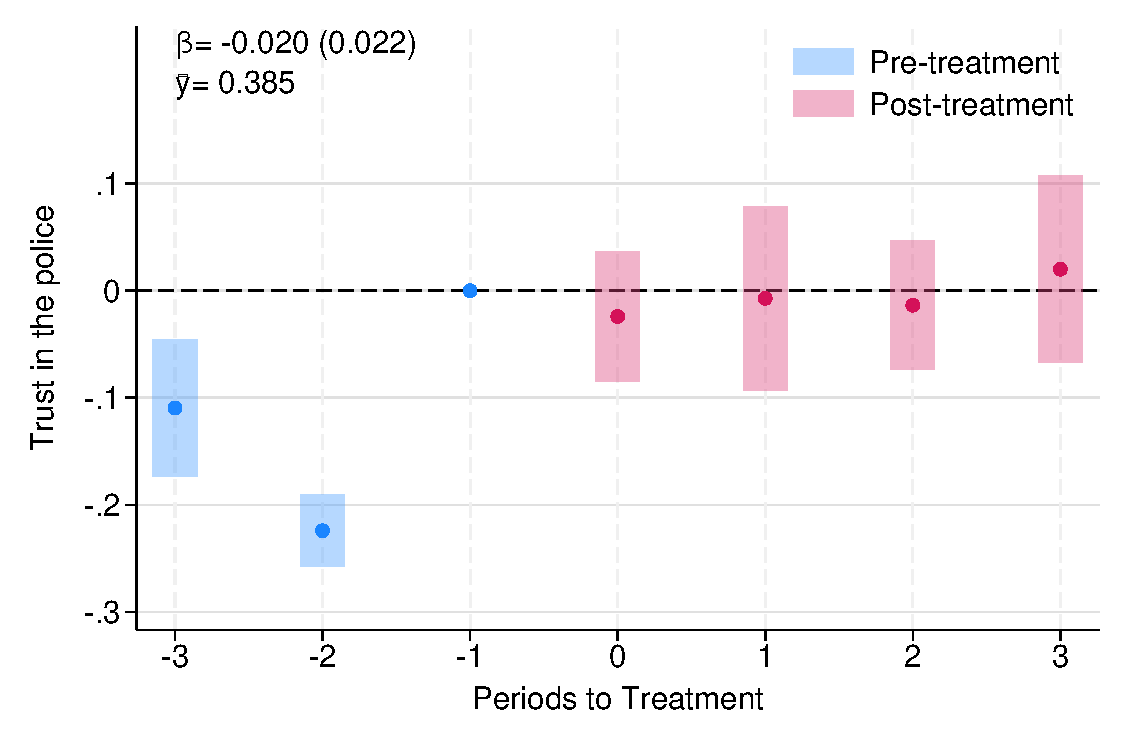
\includegraphics[width=0.98\textwidth]{../manuscript/Graphs/results_spillover_confianza_carabineros.pdf}
        \caption{Spillovers on Trust in the police}
    \end{subfigure}%
    ~
    \begin{subfigure}{0.495\textwidth}
        \centering
        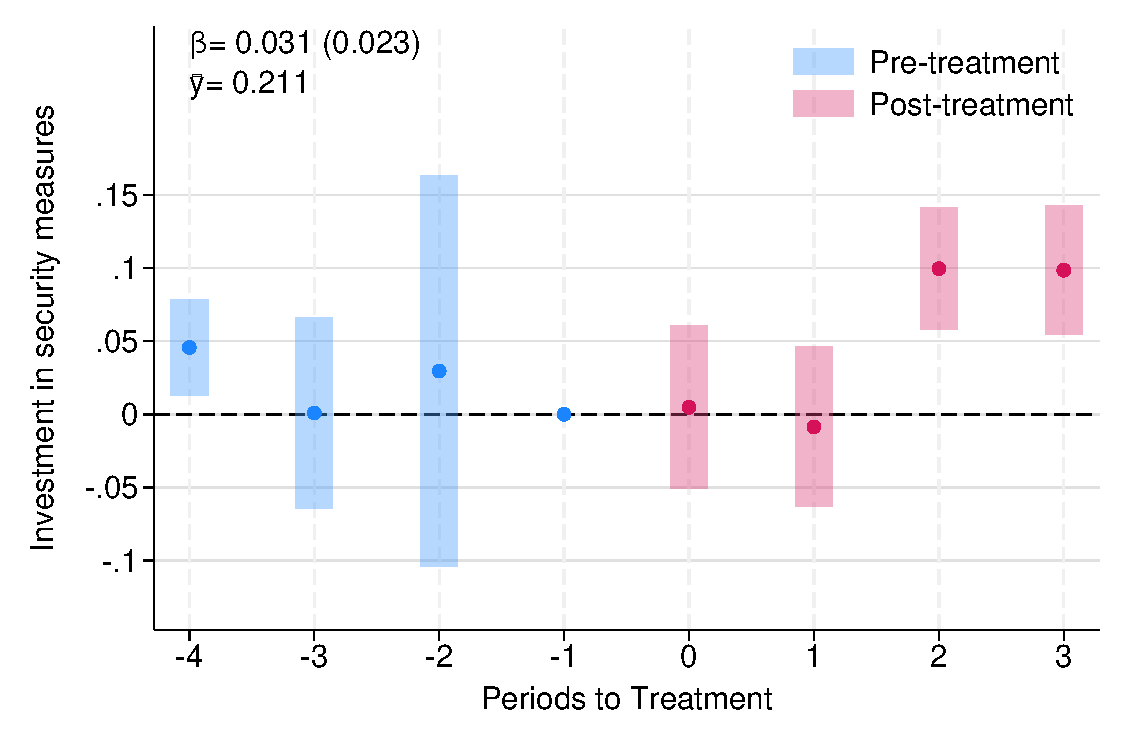
\includegraphics[width=0.98\textwidth]{../manuscript/Graphs/results_spillover_medidas_general_12.pdf}
        \caption{Spillovers on Households adopting security measures}
    \end{subfigure}
    \begin{minipage}{0.95\textwidth}
    \footnotesize
    Notes: This figure presents the geographic spillover effects of \emph{Plan Cuadrante} from early-adopting ENUSC municipalities on their late-adopting ENUSC neighbours, using the ENUSC sample. Panel (a) reports the effect of \emph{Plan Cuadrante} on the probability of household victimization in the last 12-months using the ENUSC survey. Panel (b) reports the effect on crime perception using the ENUSC survey. Panel (c) reports the effect on trust in the police using the ENUSC survey. Panel (d) reports the results on the probability of purchasing private security measures in the last twelve months using the ENUSC survey. The focal treated sample consists of six late-adopting ENUSC municipalities---Molina, Tocopilla, San Carlos, Padre Hurtado, Calera, and Limache---each assigned a spillover-onset date equal to the year its earliest-adopting ENUSC neighbour received \emph{Plan Cuadrante}: Curic\'o (2005) for Molina, Iquique (2005) for Tocopilla, Chill\'an (2007) for San Carlos, Pe\~naflor (2008) for Padre Hurtado, and Quillota (2008) for both Calera and Limache. Estimation is performed using the difference-in-differences estimator for staggered treatment adoption of \citet{Callaway}. The dots represent the estimated dynamic effects and the bars behind them denote 95\% confidence intervals. Standard errors are clustered at the municipality level. The pooled effect  and the mean of the outcome among municipalities with no treated neighbors are reported in each panel.
    \end{minipage}
\end{figure}


\clearpage


\FloatBarrier

\end{document}

